\documentclass[10pt,a4paper]{article}

\usepackage[utf8]{inputenc}		% Configuro la codificación
\input{.command.tex}
% En el siguiente archivo se configuran las variables del trabajo práctico
%% \providecommand es similar a \newcommnad, salvo que el primero ante un 
%% conflicto en la compilación, es ignorado.

% Al comienzo de un TP se debe modificar los argumentos de los comandos

\providecommand{\myTitle}{PROYECTO FINAL}
\providecommand{\mySubtitle}{Amplificador de audio de potencia Clase G alternativa}

\providecommand{\mySubject}{Diseño de Circuitos Electrónicos (86.10)}
\providecommand{\myKeywords}{UBA, Ingeniería, C2}

\providecommand{\myTutor}{-}
\providecommand{\myAuthorSurname}{Alonso, Manso, Russo, Zuccolo}
\providecommand{\myTimePeriod}{Año 2018 - 2\textsuperscript{do} Cuatrimestre}

% No es necesario modificar este %%%%%%%%%%%%%%
\providecommand{\myHeaderLogo}{header_fiuba}
%%%%%%%%%%%%%%%%%%%%%%%%%%%%%%%%%%%%%%%%%%%%%%%%

% Si se utilizan listings, definir el lenguaje aquí
\providecommand{\myLanguage}{matlab}

% Crear los integrantes del TP con el comando \PutMember donde
%%		1) Apellido, Nombre
%%		2) Número de Padrón
%%		3) E-Mail
\providecommand{\MembersOnCover}[0]
{		
		\PutMember{Alonso, Gustavo Gabriel} {96119} {gustavoalon19@gmail.com}
		\PutMember{Manso, Juan} {96133} {juanmanso@gmail.com}
		\PutMember{Russo, Nicolas Emanuel} {93211} {nicolasrusso291@gmail.com}
		\PutMember{Zuccolo, Florencia} {96628} {florenciaz618@gmail.com}
}

\providecommand{\myGroupNumber}{10}

\Pagebreaktrue		% Setea si hay un salto de página en la carátula
\Indextrue
\Siunitxtrue			% Si quiero utilizar el paquete, \siunixtrue. Si no \siunixfalse
\Todonotestrue		% Habilita/Deshabilita las To-Do Notes y las funciones \unsure, \change, \info, \improvement y \thiswillnotshow.
\Listingsfalse
\Keywordsfalse
\Putgrouptrue		% Habilita/Deshabilita el \myGroup en los headers
\Videofalse
\Tutorfalse
				% Archivo con los comandos globales como Título y autores
%Preambulo para articulo científico de LaTeX

\usepackage[a4paper,left=3cm,right=3cm,bottom=3.5cm,top=3.5cm]{geometry} 	% Configuro la geometría del papel
%\usepackage{microtype}								% Mejora el "spacing" de las palabras
\usepackage[spanish]{babel} 							% Compatibilizo los signos del español
	\addto\captionsspanish{\renewcommand{\tablename}{Tabla}}		%% Redefino nombres preestablecidos por Babel
	\addto\captionsspanish{\renewcommand{\listtablename}{Índice de tablas}}	%% y así en vez de Cuadro dirá Tabla.
\usepackage{amsmath, amsfonts, amssymb}						% Entornos matemáticos, fuentes y símbolos
\usepackage{graphicx}								% Necesario para insertar figuras
\usepackage{fancyhdr}								% Para manipular headers y footers
\usepackage[usenames,dvipsnames]{color}						% \color{color deseado} {lo que querés que tenga color}
\usepackage{subcaption}								% Permite captions del tipo 1a, 1b
\usepackage{multirow}								% Para tablas
\usepackage{multicol}
%\usepackage{slashbox}								% Cuadro divido en tablas
\usepackage{diagbox}
\usepackage{float}
\usepackage{booktabs}								% Permite hacer tablas sin separadores en el medio
\usepackage[table,xcdraw]{xcolor}						% Para colorear tablas

% Para video
\ifVideo
	\usepackage{media9}
	\addmediapath{./../reportes/}
\fi

%\usepackage{times}
%\usepackage{mathtools}
%\usepackage{upgreek} % letras griegas sin cursiva
%\usepackage{cancel}
\usepackage{rotating}
\usepackage{tikz}
\usepackage{pgfplots}
%	\pgfplotsset{compat=1.12}
	\usetikzlibrary{plotmarks}% matlab2tikz
\usepackage{grffile}% matlab2tikz 
	\usetikzlibrary{calc,patterns,decorations.pathmorphing,decorations.markings}

\ifListings
	\usepackage{listings}

	\providecommand{\lstinputpath}[1]{\lstset{inputpath=#1}}

%	\input{.lst_default.tex}
	\input{.lst_matlab.tex}
%	\input{.lst_c.tex}
%	\input{.lst_c++.tex}
	
% 	\input{.lst_pseudocode.tex}


\fi

\ifSiunitx
\usepackage{siunitx}											% Unidades: \SI {cantidad} {\unidad} (necesita texlive-science)
	\sisetup{load-configurations = abbreviations}							% Habilita poner \cm en vez de \centi\metre
	\sisetup{output-decimal-marker = {,}}									% Cambia los puntos decimales por comas
	\sisetup{per-mode = fraction}											% Pone las unidades como fracción
	\sisetup{quotient-mode = fraction}										
\fi


\ifTodonotes
\usepackage{xargs}
\usepackage[colorinlistoftodos,prependcaption,textsize=tiny]{todonotes}


	\newcommandx{\Juan}[2][1=]{\todo[linecolor=red,backgroundcolor=red!25,bordercolor=red,#1]{#2}}
	\newcommandx{\Flor}[2][1=]{\todo[linecolor=blue,backgroundcolor=blue!25,bordercolor=blue,#1]{#2}}
	\newcommandx{\Gus}[2][1=]{\todo[linecolor=green,backgroundcolor=green!25,bordercolor=green,#1]{#2}} % OliveGreen
	\newcommandx{\Nico}[2][1=]{\todo[linecolor=yellow,backgroundcolor=yellow!25,bordercolor=yellow,#1]{#2}}
	\newcommandx{\thiswillnotshow}[2][1=]{\todo[disable,#1]{#2}}
\fi


\usepackage{placeins}														
		\let\Oldsection\section												%% Permite que los flotantes (como figuras) no aparescan
	\renewcommand{\section}{\FloatBarrier\Oldsection}						%% antes o después de su sección correspondiente.
		\let\Oldsubsection\subsection
	\renewcommand{\subsection}{\FloatBarrier\Oldsubsection}		
		\let\Oldsubsubsection\subsubsection
	\renewcommand{\subsubsection}{\FloatBarrier\Oldsubsubsection}
\usepackage{hyperref}														% Debe ser agregado al final del preambulo

\hypersetup
{    bookmarks=true,         % show bookmarks bar?
     unicode=false,          % non-Latin characters in Acrobat’s bookmarks
     pdftoolbar=true,        % show Acrobat’s toolbar?
     pdfmenubar=true,        % show Acrobat’s menu?
     pdffitwindow=false,     % window fit to page when opened
     pdftitle={\myTitle},    		 % title
     pdfauthor={\myAuthorSurname},   % author
	 pdfcreator={\myAuthorSurname},	 % creator = author
     pdfsubject={\mySubject},		 % subject of the document
     pdfkeywords={\myKeywords},
     colorlinks=true,        % false: boxed links; true: colored links
     linkcolor=black,        % color of internal links (change box color with linkbordercolor)
     citecolor=black,        % color of links to bibliography
     filecolor=magenta,      % color of file links
     urlcolor=cyan           % color of external links
}

%Configuro la pagina con los encabezaos y pies de paginas
\pagestyle{fancy}										% Para agregar encabezados y pie de paginas	
%\lhead{\mySubject}										% Encabezado izquierdo
\lhead{DCE (86.10)}
\rhead{\includegraphics[scale=0.15]{\myHeaderLogo}} 	% Encabezado derecho (logo de la FIUBA)	
\ifPutgroup
\chead{\texttt{Grupo Nº\myGroupNumber} \\ \textit{\footnotesize{\myTimePeriod}}}
\fi				

%% Este archivo contiene las funciones auxiliares para escribir en LaTeX
%% Dichas funciones resuelven la sintaxis de generar figuras, por ejemplo,
%% dejando el código más compacto y facilitando la corrección del mismo.



% Comando para graficar eps. 1er arg, escala. 2do, ruta. 3ro, caption. 4to, label.
\providecommand{\HgraficarEPS}[4]{
			\begin{figure}[h!]
				\centering
					\scalebox{#1}{\input{#2}}
					\caption{#3}
					\label{#4}
			\end{figure}

}

\providecommand{\HgraficarPNG}[4]{
			\begin{figure}[h!]
				\centering
					\includegraphics[scale=#1]{#2}
					\caption{#3}
					\label{#4}
			\end{figure}

}


% Comando para graficar eps en el lugar previsto.
\providecommand{\graficarEPS}[4]{
			\begin{figure}[h]
				\centering
					\scalebox{#1}{\input{#2}}
					\caption{#3}
					\label{#4}
			\end{figure}

}

\providecommand{\graficarPNG}[4]{
			\begin{figure}[h]
				\centering
					\includegraphics[scale=#1]{#2}
					\caption{#3}
					\label{#4}
			\end{figure}

}

\providecommand{\underuparrow}[2]{\underset{\underset{#2} \uparrow} #1 }

\providecommand{\cltext}[2]{\color{#1}{\huge{#2}}}
\providecommand{\cstext}[2]{\color{#1}{\large{#2}}}

\providecommand{\lsi}[1]{\large\si{#1}}
\providecommand{\lsio}[0]{\large\si{\ohm}}
\providecommand{\lsiv}[0]{\large\si{\volt}}
\providecommand{\lsia}[0]{\large\si{\ampere}}
\providecommand{\lSI}[2]{\large\SI{#1}{#2}}


		% Se proveen un conjunto de funciones extras

% Defino el path de los includegraphics
\graphicspath{{./Figuras/}}		% Directorio que contiene los graficos

% Defino el path para los input de .tex y de .eps
\makeatletter
\def\input@path{{./Figuras/}{./Secciones/}{./Cover_page/}{../Octave/graficos/}}
\makeatother

% Defino el path del listings
\ifListings
%% Cambiar el nombre de la carpeta si se utilizan Listings
	\lstinputpath{{../Octave/}}
\fi

\definecolor{myred}{rgb}{0.5,0,0}
\definecolor{mygreen}{rgb}{0,0.5,0}



\begin{document}
		% Carátula (formal o simple,_formal o _simple respectivamente) con Resumen
		% incluido e Índice (si es necesario configurar en config.tex) del informe
		\begin{titlepage}
	
		\thispagestyle{empty}

		\begin{center}
			
\includegraphics[scale=0.3]{fiuba}\\
			\large{\textsc{Universidad de Buenos Aires}}\\
			\large{\textsc{Facultad De Ingeniería}}\\
			\small{\myTimePeriod}
		\end{center}

		\vfill

		\begin{center}
			\Large{\underline{\textsc{\mySubject}}}
		\end{center}

		\vfill

		\begin{tabbing}
			\hspace{2cm}\=\+\myTitle\\
				TEMA: \mySubtitle\\
				TUTOR: \myTutor\\
				FECHA: \today\\
				\ifPutgroup
				GRUPO: \texttt{\myGroupNumber}\\
				\fi

			\\
				\MembersHeader
				\MembersOnCover	
		\end{tabbing}

		\begin{abstract}
			% Ejemplo de Resumen
%% MANTENER EL NOMBRE %%
El presente informe expone el proceso de diseño y construcción de un equipo electrónico partiendo de ciertas especificaciones.

		\end{abstract}

	\ifKeywords
		\begin{center}
			\emph{Palabras Clave: \myKeywords}
		\end{center}
	\fi	

		\vfill
	
\end{titlepage}

\ifPagebreak
	\thispagestyle{empty}
	\ifIndex
		\tableofcontents
%		\listoffigures
%		\listoftables
	\fi

	\pagebreak
\fi


	\setcounter{page}{1}

	\part{Introducción}\label{part:intro}

		\section{Objetivos}\label{sec:obj}
			
%	Las señales de audio tienen una relación de pico/valor medio elevado, estando la mayor parte del tiempo en valores bajos.

	El trabajo consiste en la confección de un amplificador de audio tanto en su forma teórica como práctica; una vez determinados los valores de los componentes a partir de un análisis teórico y posterior simulación, se procede a armar el mismo de forma discreta y realizar distintas mediciones para compararlas con los datos previamente obtenidos. \\ 

	A continuación se analiza su comportamiento y se detalla cada parte del circuito, explicando el propósito de cada componente y el valor elegido para su óptimo funcionamiento.


		\section{Requerimientos}\label{sec:req}
			El amplificador de audio a diseñar debe cumplir las siguientes especificaciones:

\begin{itemize}
	\item Topología de la etapa de salida Clase G alternativa.
	\item Tensión de alimentación $\pm \SI{30}{\volt}$ con una variación de \SI{5}{\volt}.
%	\item Potencia de salida nominal de \SI{39}{\watt} sobre \SI{8}{\ohm} a \SI{1}{\kilo\hertz} con $THD<0,02\%$.
	\item Potencia de salida nominal de \SI{40}{\watt} sobre \SI{8}{\ohm} a \SI{1}{\kilo\hertz} con $THD<0,02\%$.
	\item Potencia de salida a \SI{1}{\watt} sobre \SI{8}{\ohm} con $THD<0,01\%$. 
	\item Respuesta en frecuencia \SI{20}{\hertz} a \SI{20}{\kilo\hertz}.
	\item Tensión de \textit{offset} en la salida en continua \SI{5}{\milli\volt}.
	\item \textit{Slew Rate} $\approx$ \SI{10}{\volt\per\micro\second}.
	\item Distorsión IMD cercana al 1\%.
	\item Impedancia de entrada del orden de \SI{100}{\kilo\ohm}.
	\item Impedancia de salida del orden de los \SI{}{\milli\ohm}.
	\item Factor de amortiguamiento del orden de 500.
	\item Margen de fase mayor que \SI{45}{\degree}.
\end{itemize}


%
%	\begin{table}[h!]
%		\centering
%		\begin{tabular}{*{2}{c}}
%			\toprule
%			Tipo de especificación & Valor\\
%			\midrule
%			$\pm V_{CC}$			& $\pm$\SI{30}{\V} con tolerancia de $\pm$\SI{1}{\V}\\
%			Respuesta en frecuencia		& \SI{20}{\Hz} a \SI{20}{\kHz}\\
%			Ancho de banda de potencia	& \SI{20}{\Hz} a \SI{20}{\kHz}\\
%			Rango dinámico			& Mínimo = \SI{40}{\dB} para reproducir vinilos\\
%			Distorsión armónica total (\emph{THD})& Mínimo = 1\%\\
%			Relación señal a ruido (\emph{SNR})& \SI{60}{\dB}\\
%			Sensibilidad			& 1 Vrms\\
%			\emph{Slew Rate}		& \SI{15}{\micro\V\per\second}\\
%			\emph{DC Offset}		& Máximo = \SI{1}{\mV}\\
%			Impedancia de entrada		& $R_{in} \approx \SI{10}{\kilo\ohm}$\\
%			Impedancia de salida		& $R_{out} \approx \SI{10}{\milli\ohm}$\\
%			Factor de amortiguamiento	& $FA \approx 500$\\
%			Margen de fase			& $\varphi_m= \SI{60}{\degree}$\\
%			Margen de ganancia		& Sólo que sea positivo para que sea estable\\
%			Potencia nominal (sin exigir mucho) & Suponiendo que no le dan con todo, todo el tiempo\\
%			Potencia máxima			& Para 25V\\
%			\bottomrule
%		\end{tabular}
%	\end{table}
%
%
%	Poner las bases de los comporadares en Vout en vez de la salida de la 2nda.
%	Bajar el Vth
%	Ver qué queda en la corriente de salida a partir de la distorsión
%	Bajar la resistencia de emisor del comparador para tener menos corriente.
%	Ver las corrientes que necesitan los tr de salida.
%	
%


	\part{Diseño conceptual}\label{part:concept}

		\section{Diagrama en bloques}\label{sec:bloques}
			\HgraficarEPS{0.5}{bloques}{Diagrama en bloques}{fig.bloques}

	\Juan{Tal vez hacer los bloques que marcamos después más adelante.. ¿?}
	En la Figura \ref{fig.bloques} se muestran los bloques principales de un amplificador de audio, que consiste en tres etapas, cada una de ellas con cierta funcionalidad.

\begin{itemize}
	\item \textbf{Comparador:} es un amplificador de transconductancia. Su entrada es una tensión diferencial y su salida una corriente.
	\item \textbf{Amplificación de tensión (VAS):} amplificador de transimpedancia (la entrada es corriente y la salida tensión).
	\item \textbf{Separador (\textit{Buffer}):} es un adaptador de impedancias con ganancia de tensión unitaria y de corriente elevada. Entrega la potencia a la carga.
\end{itemize}


		\section{Funcionamiento general}\label{sec:func_gral} % Acá se explican los bloques
			% Acá se explican los bloques



		\section{Alternativas de diseño}\label{sec:alt}
			
	A partir del análisis realizado sobre el amplificador \emph{Turner 730} se ve que una implementación posible de la etapa de entrada es un emisor común. Se considera la alternativa de utilizar un par diferencial. A pesar de la dificultad propia del balanceo del par diferencial (selección de componentes similares, cargas, fuentes de corriente, etc.), las ventajas del mismo son mucho mayores al emisor común que se utilizaba en los \emph{70} dada la escasez de transistores. Entre las ventajas se destaca la baja tensión de corrimiento $V_{off}$; las corrientes no fluyen por el lazo de realimentación; linealidad superior a la entrada con 1 solo transistor; buen acoplamiento térmico.\\

	Por otro lado, para la implementación de los comparadores encargados de la conmutación de las fuentes externas de la etapa de salida clase G alternativa se consideraron amplificadores operaciones y un par diferencial discreto. Los amplificadores operacionales facilitan la implementación del circuito, pero dificulta la producción dada la escasez o falta de provisión de los mismos. La solución es realizar un diseño sencillo con transistores discretos de un par diferencial que a su vez es más ajustable dado que el diseño es propio y se puede personalizar el comparador a la medida de las necesidades del dispositivo.\\

	\Juan{Qué alternativa sería 'Separación de VAS con corriente de polarización de etapa de salida (separada por un capacitor)'?}


%	- Comparadores: utilización de operacionales en vez del par diferencial discreto. Componentes difíciles de conseguir
%	
%	- Separación de VAS con corriente de polarizacion de etapa de salida (separada por un capacitor)
%	
%	- Multiplicador de VBE doble.
%	
%	\Juan{Hacer la tabla en internet}
%	\begin{table}[h!]
%		\centering
%		\begin{tabular}{*{4}{c}}
%			\toprule
%			Etapa                                  & Alternativa & Ventajas & Desventajas \\ 
%			\midrule
%			\multirow{2}{*}{Comparador de entrada} &             &          &             \\ %\cmidrule(l){2-4} 
%	&\colortab Par diferencial             &          &             \\
%			\midrule
%			\multirow{2}{*}{VAS} &             &          &             \\ %\cmidrule(l){2-4} 
%			                                       &             &          &             \\
%			\midrule
%			\multirow{2}{*}{Etapa de salida} & Clase G            &          &             \\ %\cmidrule(l){2-4} 
%							 &  \colortab Clase G alternativa           & \colortab Menor distorsión	& \colortab Diseño más complejo\\
%			\midrule
%			\multirow{2}{*}{Fuente de corriente} & FES	& Simple	& Error apreciable, malo bajo ripple             \\ %\cmidrule(l){2-4} 
%							&\colortab FES corregida	& \colortab Más estable vs ripple	& \colortab Más componentes \\
%			\bottomrule
%		\end{tabular}
%	\end{table}
%	
%	Carga FES versus bootstrap en el VAS. El bootstrap es dependiente de la ganancia de la etapa de salida y esta puede variar por la carga utilizada. Otra contra es la corriente de polarizacion varia segun varie la fuente 
%	Cascode versus colector común pre emisor común. Cascode permite VAS con alto beta y buena respuesta en frecuencia. Colector común es más simple y facil de diseñar.


	\part{Diseño y análisis teórico}\label{part:teo}
		
	En la Figura \ref{fig.cto_completo} se muestra el circuito amplificador de potencia completo, donde se han identificado en línea punteada los bloques que conforman el amplificador. Se debe destacar que dicha selección de bloques es aproximada, ya que las etapas se encuentran relacionadas, es decir que comparten componentes y una etapa sin la otra podría no operar correctamente. A continuación se detallará el funcionamiento de la implementación de cada bloque, comenzando por la etapa de salida.

\begin{figure}[H]
	%\centering
	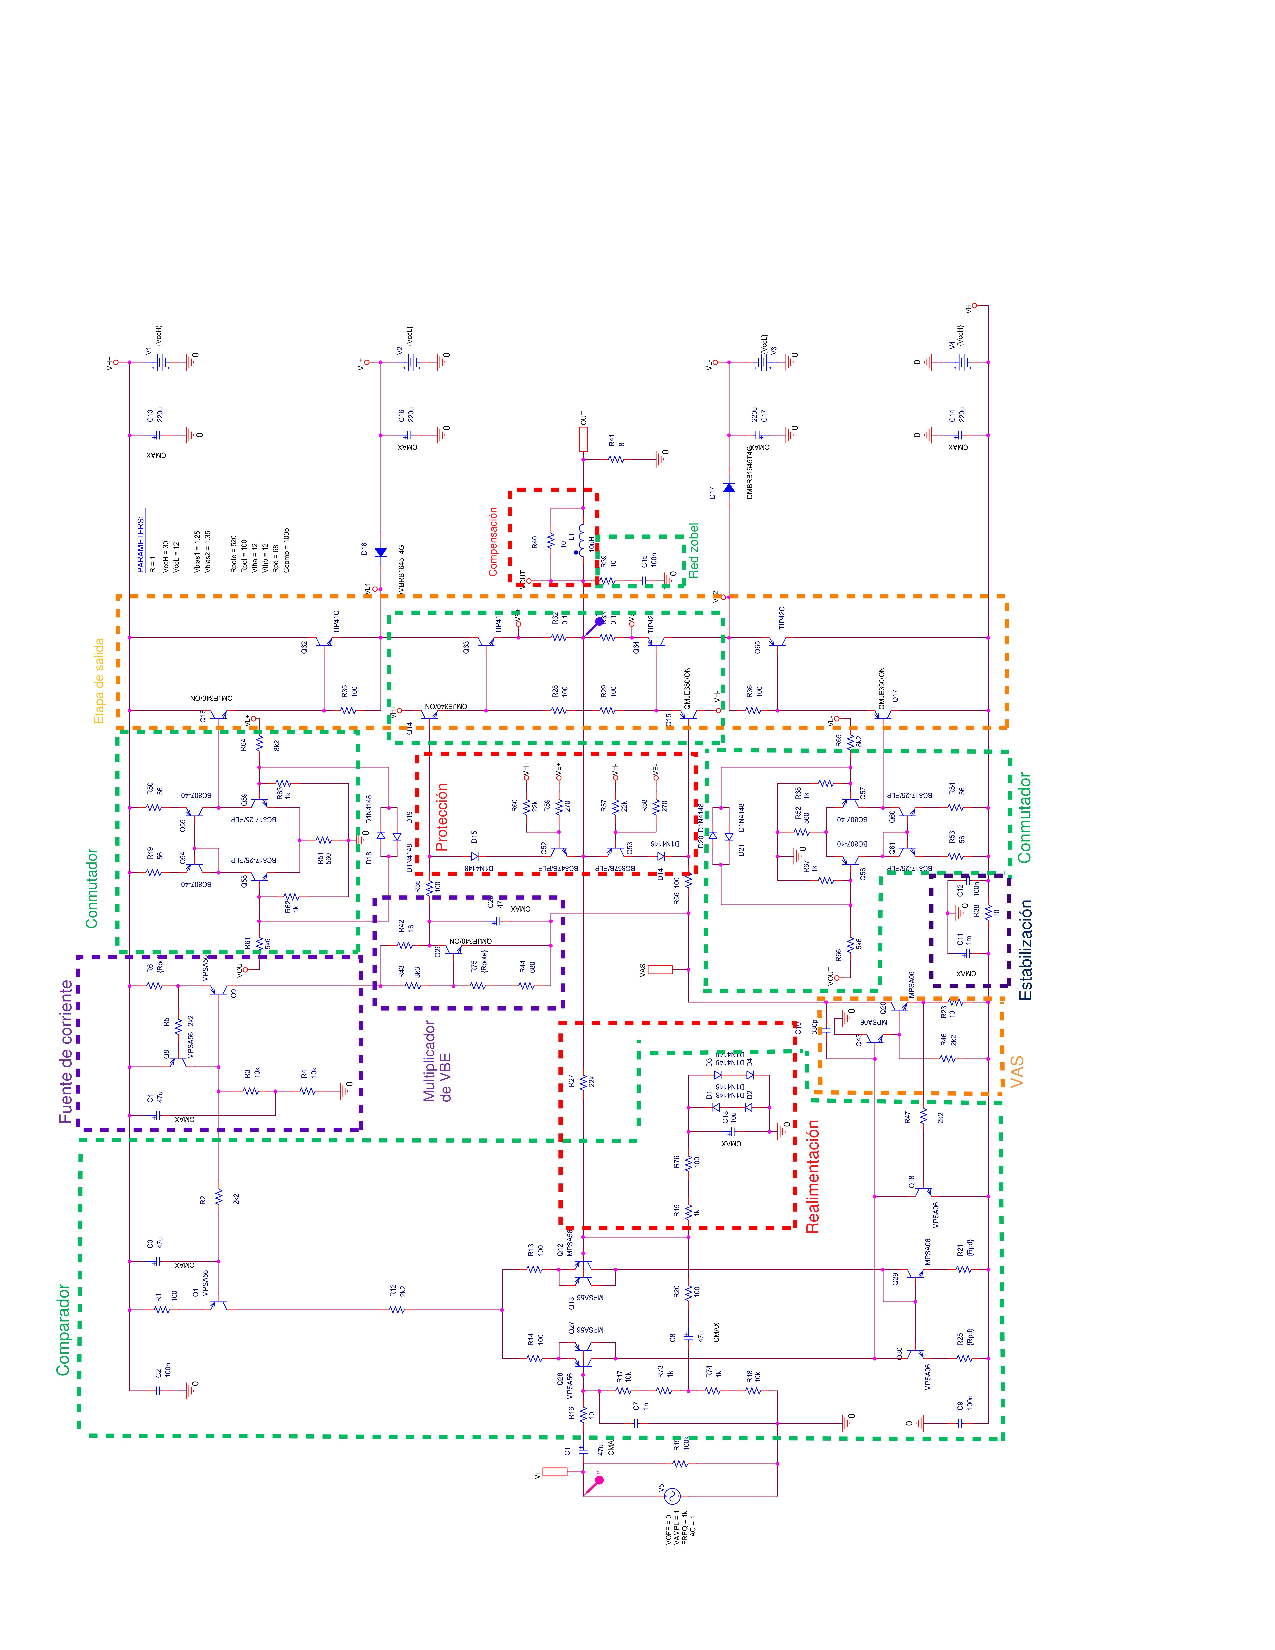
\includegraphics[angle=-90,width=1.1\textwidth, trim = 0.5cm 3.0cm 4cm 4cm]{esquema2.pdf}
	\caption{Circuito completo.}
	\label{fig.cto_completo}
\end{figure}

	% Acá se introduce al cto propuesto y después se analiza

		\section{Etapa de salida}
				La etapa de salida clase G se caracteriza principalmente por el manejo eficiente de potencia debido a que conmuta la tensión de alimentación entre dos niveles según lo requiera la señal de entrada.

	En la figura se muestra un esquema básico de la topología, denominada Clase G alternativa.  Los transistores $Q_1$ y $Q_2$ conforman la etapa interior que opera en clase B, siendo $Q3$ y $Q4$ los \textit{drivers} y $R1$ la resistencia de emisor compartida. 

	\begin{figure}[H]
		\centering
		\scalebox{0.5}{% XCircuit output "salida.tex" for LaTeX input from salida.eps
\def\putbox#1#2#3#4{\makebox[0in][l]{\makebox[#1][l]{}\raisebox{\baselineskip}[0in][0in]{\raisebox{#2}[0in][0in]{\scalebox{#3}{#4}}}}}
\def\rightbox#1{\makebox[0in][r]{#1}}
\def\centbox#1{\makebox[0in]{#1}}
\def\topbox#1{\raisebox{-0.60\baselineskip}[0in][0in]{#1}}
\def\midbox#1{\raisebox{-0.20\baselineskip}[0in][0in]{#1}}
   \scalebox{1}{
   \normalsize
   \parbox{6.61458in}{
   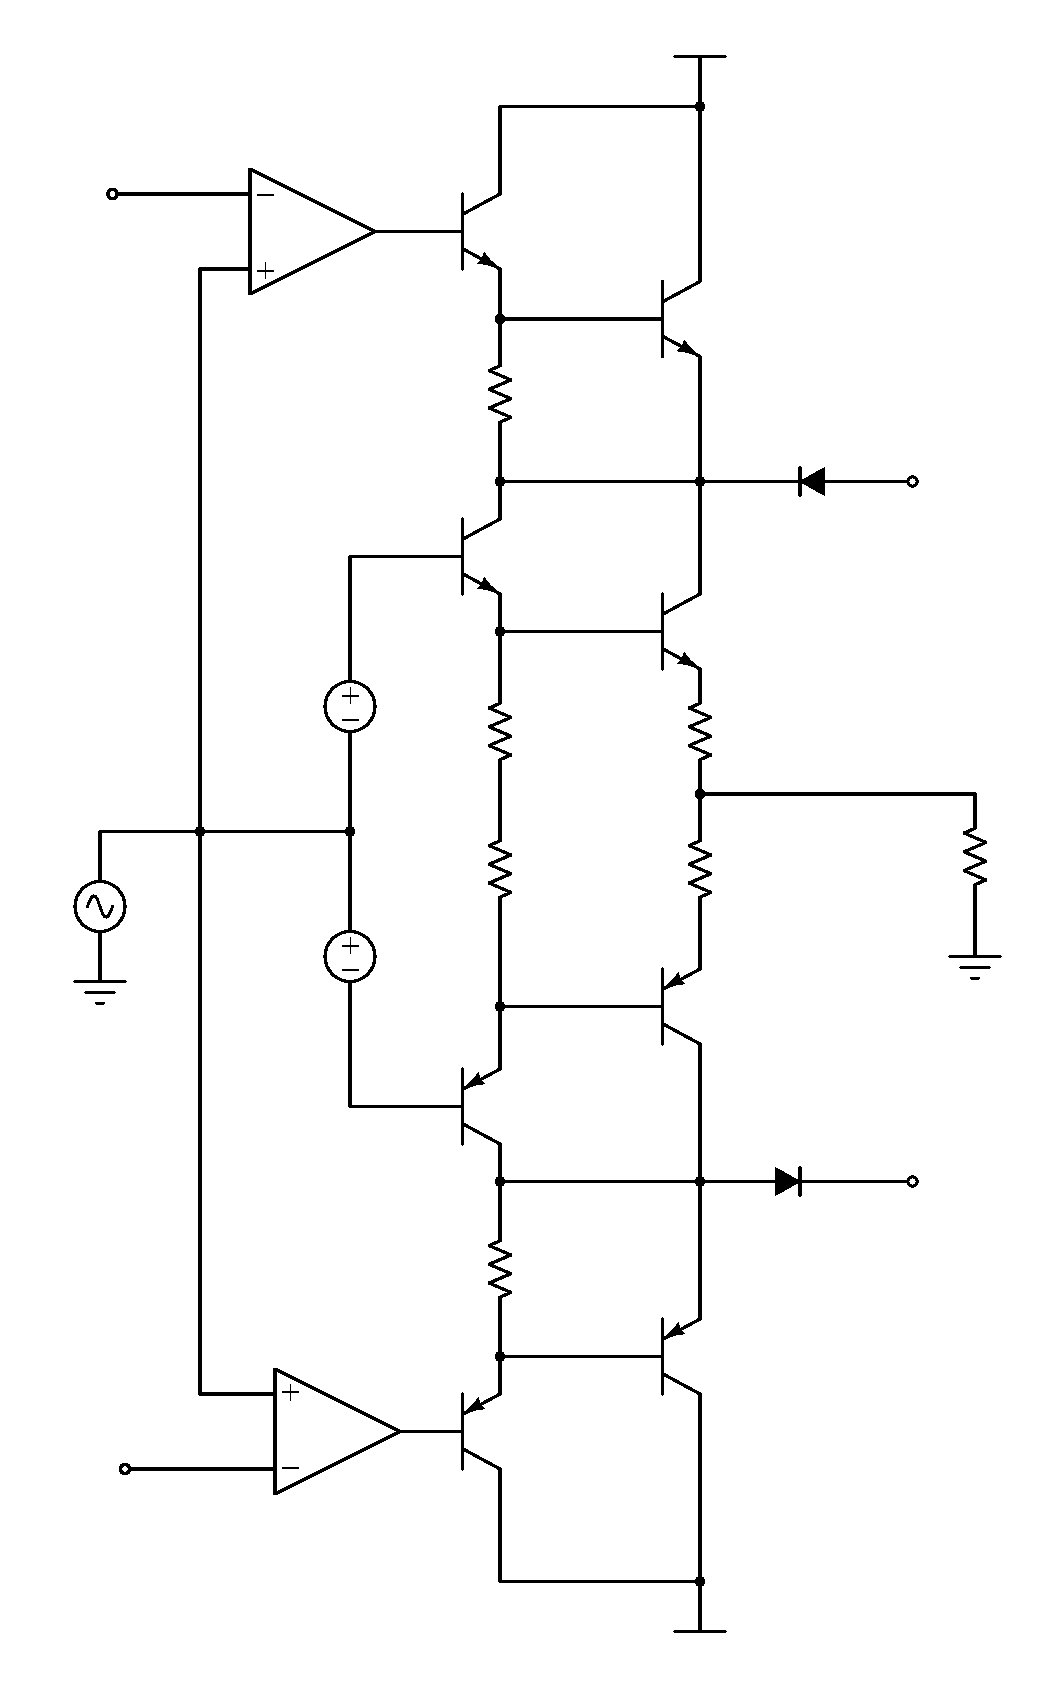
\includegraphics[scale=1]{salida}\\
   % translate x=800 y=1584 scale 0.38
   \putbox{1.39in}{6.39in}{1.20}{Vbias1}%
   \putbox{1.39in}{4.81in}{1.20}{Vbias2}%
   \putbox{5.89in}{5.39in}{1.20}{RL}%
   \putbox{4.72in}{6.22in}{1.20}{Re}%
   \putbox{4.72in}{5.31in}{1.20}{Re}%
   \putbox{4.47in}{6.89in}{1.20}{Q63}%
   \putbox{4.47in}{4.39in}{1.20}{Q64}%
   \putbox{3.14in}{7.47in}{1.20}{Q14}%
   \putbox{3.14in}{3.72in}{1.20}{Q15}%
   \putbox{3.14in}{9.56in}{1.20}{Q16}%
   \putbox{4.47in}{9.06in}{1.20}{Q62}%
   \putbox{3.14in}{1.56in}{1.20}{Q17}%
   \putbox{4.47in}{2.06in}{1.20}{Q65}%
   \putbox{0.14in}{1.31in}{1.20}{Vth-}%
   \putbox{0.06in}{9.81in}{1.20}{Vth+}%
   \putbox{4.22in}{0.06in}{1.20}{-VccH}%
   \putbox{4.22in}{10.89in}{1.20}{+VccH}%
   \putbox{6.06in}{7.89in}{1.20}{VccL+}%
   \putbox{6.06in}{3.22in}{1.20}{-VccL}%
   } % close 'parbox'
   } % close 'scalebox'
   \vspace{-\baselineskip} % this is not necessary, but looks better
}
		\caption{Etapa de salida.}
		\label{fig.salida}
	\end{figure}

	Los comparadores se encuentran conectados a la señal de entrada y a una tensión umbral Vth como referencia. Cuando la señal de entrada excede la tensión $+Vth$, el comparador (superior) hace que los transistores $Q5$ y $Q6$ se polaricen en saturación. Es decir que actúan como una llave que activa la alimentación $VccH$. A su vez el diodo $D1$ quedará polarizado en inversa ya que la tensión en el cátodo es $+VccH$, mayor que la tensión de ánodo $VccL$. Por lo tanto, el circuito queda alimentado solo mediante $+VccH$ y la potencia es manejada por dos transistores $Q6$ y $Q1$.

	De forma análoga funcionan el comparador $C2$, $Q7$, $Q8$ y $D2$ para el semicilo negativo de la señal de entrada.

	Las tensiones $Vbias1$ y $Vbias2$ permiten \textit{prepolarizar} a los transistores $Q1$ y $Q2$ con el fin de atenuar la distorsión de cruce por cero. Se deben ajustar de forma tal que la corriente de la malla de salida sea aproximadamente igual en el colector de ambos transistores ($Q1$ y $Q2$). Asimismo se debe considerar que si $ICQ$ es muy elevada se desperdicia potencia, y si es muy pequeña se obtendrá una distorsión de cruce por cero apreciable. 


\subsection{Multiplicador de $V_{BE}$}

	\begin{figure}[H]
		\centering
		\scalebox{0.5}{% XCircuit output "multiplicador.tex" for LaTeX input from multiplicador.eps
\def\putbox#1#2#3#4{\makebox[0in][l]{\makebox[#1][l]{}\raisebox{\baselineskip}[0in][0in]{\raisebox{#2}[0in][0in]{\scalebox{#3}{#4}}}}}
\def\rightbox#1{\makebox[0in][r]{#1}}
\def\centbox#1{\makebox[0in]{#1}}
\def\topbox#1{\raisebox{-0.60\baselineskip}[0in][0in]{#1}}
\def\midbox#1{\raisebox{-0.20\baselineskip}[0in][0in]{#1}}
   \scalebox{1}{
   \normalsize
   \parbox{4.18229in}{
   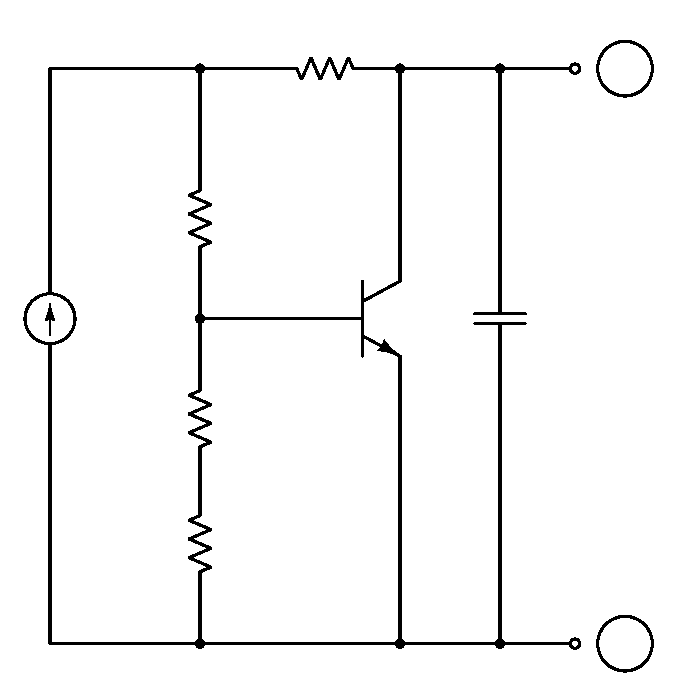
\includegraphics[scale=1]{multiplicador}\\
   % translate x=672 y=611 scale 0.38
   \putbox{3.56in}{2.32in}{1.20}{C20}%
   \putbox{2.47in}{2.32in}{1.20}{Q26}%
   \putbox{0.56in}{3.07in}{1.20}{R43}%
   \putbox{0.72in}{1.74in}{1.20}{Rp}%
   \putbox{0.64in}{0.82in}{1.20}{R44}%
   \putbox{1.89in}{4.24in}{1.20}{R42}%
   \putbox{4.06in}{4.07in}{1.20}{\centbox{\midbox{1,1}}}%
   \putbox{4.06in}{0.24in}{1.20}{\centbox{\midbox{-1,1}}}%
   \putbox{0.47in}{2.32in}{1.20}{Ipol}%
   \putbox{1.97in}{3.74in}{1.20}{$10 \Omega$}%
   \putbox{1.47in}{3.07in}{1.20}{$3,3 k\Omega$}%
   \putbox{1.39in}{0.82in}{1.20}{$680 \Omega$}%
   \putbox{1.39in}{1.65in}{1.20}{$1 k\Omega$}%
   } % close 'parbox'
   } % close 'scalebox'
   \vspace{-\baselineskip} % this is not necessary, but looks better
}
		\caption{Multiplicador de $V_{BE}$.}
		\label{fig.multiplicador}
	\end{figure}

	La resistencia $R_{3M}$ se anexa para mejorar la independencia de la tensión $V_{BE}$ con la corriente de polarización.

	\begin{equation}
		\centering
		V_M = \left( \frac{R_{1M}}{R_{1M} + R_{2M}} +1 \right) \cdot V_{BE} - I_C \cdot R_{3M} \approx  \left( \frac{R_{1M}}{R_{1M} + R_{2M}} +1 \right) \cdot V_{BE}
	\end{equation}

	 Considerando un valor de $V_{BE} \approx \SI{0.5}{\volt}$

	 \begin{equation}
	 	\centering
		\frac{\SI{2.2}{\volt}}{\SI{0.5}{\volt}} -1 = \frac{R_{1M}}{R_{2M}} \implies \boxed{R_{1M} = \num{3,4} \cdot R_{2M}}
	\end{equation}
	Se eligen los resistores comerciales $R_{1M} = \SI{3.3}{\kilo\ohm}$, $R_{2M} = \SI{680}{\ohm}$ y un potenciómetro de $\SI{1}{\kilo\ohm}$. 


\subsection{Comparadores}

	\begin{figure}[H]
		\centering
		\scalebox{0.5}{% XCircuit output "comparador.tex" for LaTeX input from comparador.eps
\def\putbox#1#2#3#4{\makebox[0in][l]{\makebox[#1][l]{}\raisebox{\baselineskip}[0in][0in]{\raisebox{#2}[0in][0in]{\scalebox{#3}{#4}}}}}
\def\rightbox#1{\makebox[0in][r]{#1}}
\def\centbox#1{\makebox[0in]{#1}}
\def\topbox#1{\raisebox{-0.60\baselineskip}[0in][0in]{#1}}
\def\midbox#1{\raisebox{-0.20\baselineskip}[0in][0in]{#1}}
   \scalebox{1}{
   \normalsize
   \parbox{7.08333in}{
   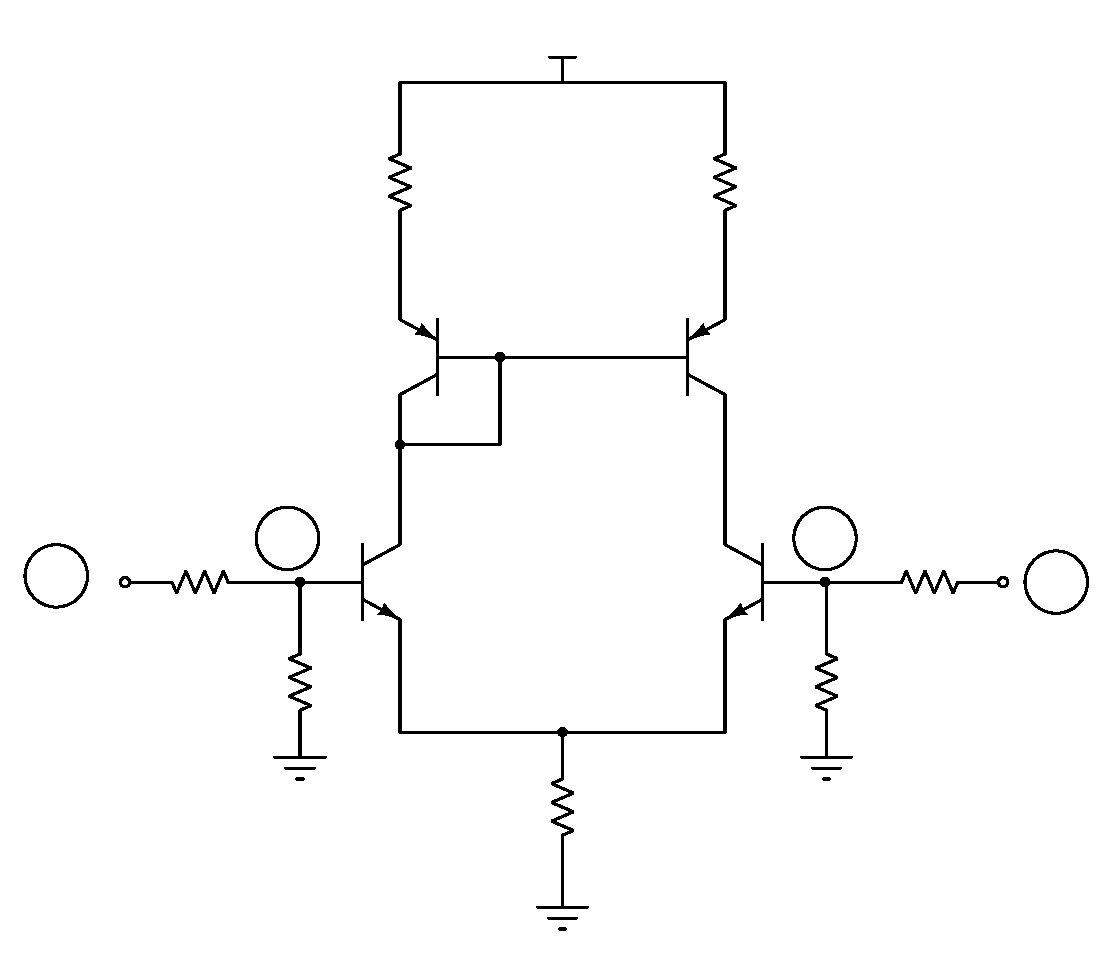
\includegraphics[scale=1]{comparador}\\
   % translate x=928 y=636 scale 0.38
   \putbox{2.58in}{2.33in}{1.20}{Q9}%
   \putbox{4.45in}{2.29in}{1.20}{Q10}%
   \putbox{2.37in}{3.81in}{1.20}{Q11}%
   \putbox{4.66in}{3.81in}{1.20}{Q12}%
   \putbox{3.35in}{5.95in}{1.20}{+VccH}%
   \putbox{0.14in}{2.33in}{1.20}{Vo}%
   \putbox{3.18in}{0.83in}{1.20}{Rec}%
   \putbox{1.10in}{2.54in}{1.20}{R1}%
   \putbox{1.47in}{1.70in}{1.20}{R2}%
   \putbox{5.97in}{2.49in}{1.20}{R3}%
   \putbox{5.01in}{1.66in}{1.20}{R4}%
   \putbox{2.18in}{5.04in}{1.20}{R5}%
   \putbox{4.35in}{4.99in}{1.20}{R6}%
   \putbox{1.64in}{2.58in}{1.20}{Vo'}%
   \putbox{5.18in}{2.58in}{1.20}{Vth'}%
   \putbox{6.76in}{2.33in}{1.20}{Vth}%
   \putbox{2.76in}{5.04in}{1.20}{56}%
   \putbox{4.93in}{5.04in}{1.20}{56}%
   \putbox{1.10in}{2.08in}{1.20}{5,6k}%
   \putbox{2.06in}{1.70in}{1.20}{1k}%
   \putbox{5.51in}{1.70in}{1.20}{1k}%
   \putbox{5.89in}{2.08in}{1.20}{8,2k}%
   \putbox{3.81in}{0.83in}{1.20}{560}%
   } % close 'parbox'
   } % close 'scalebox'
   \vspace{-\baselineskip} % this is not necessary, but looks better
}
		\caption{Comparador.}
		\label{fig.comparador}
	\end{figure}

	Se propone la configuración de par diferencial de la figura para implementar los comparadores. Se utiliza una fuente de corriente espejo para lograr mayor estabilidad. En vez de comparar con la señal proveniente de la etapa VAS, se compara con la señal de salida $V_{o}$ para evitar cargar la VAS con la resistencia de entrada que presenta el par diferencial ($2\cdot r_\pi$). La señal de salida no resulta alterada por tratarse de un colector común que es separador de impedancias.
	Por otra parte, es difícil lograr en la práctica que los transistores que conforman el par diferencial manejen una excursión de tensión de hasta \SI{30}{\volt}, por lo que se utiliza un divisor resistivo en ambas bases de los transistores para atenuar la amplitud de tensión. Es conveniente que la tensión de referencia $Vth'$ sea levemente menor que la prevista con el fin de contrarrestar el retardo de tiempo del comparador.

\begin{equation}
	\centering
	V_{th}' = V_{th} \cdot \frac{R_4}{R_4 + R_3} \implies \SI{1.5}{\volt} = \SI{12}{\volt} \cdot \frac{R_4}{R_4 + R_3} \implies \boxed{R_3 = 7 \cdot R_4}
\end{equation}

\begin{equation}
	\centering
	V_o' = V_o \cdot \frac{R_2}{R_2 + R_1} \implies \SI{2}{\volt} = \SI{12}{\volt} \cdot \frac{R_2}{R_2 + R_1} \implies \boxed{R_1 = 5 \cdot R_2}
	\end{equation}

	El valor de la resistencia de emisor $R_{ec}$ se elige en función de la máxima tensión posible en $V_o$ y la corriente que circularía en reposo. Con $R_ec = \SI{500}{\ohm}$ se obtiene:

	\begin{equation}
		\centering
		I_{e,max} = \frac{ \SI{1.3}{\volt} }{ \SI{500}{\ohm} } = \SI{2.6}{\milli\ampere}
	\end{equation}

	\begin{equation}
		I_{e,pol} = \frac{ \SI{0.8}{\volt} }{ \SI{500}{\ohm} } = \SI{1.6}{\milli\ampere} \implies \SI{1.28}{\milli\watt}
	\end{equation}



		\section{Amplificación de tensión}
				\graficarEPS{0.6}{vas}{Topología propuesta para la etapa VAS.}{fig:topologia_vas}
	Suponinedo una ganancia baja en la primer etapa del circuito implementada como un par diferencial, las capacidades reflejadas por \emph{Miller} son menores implicando constantes de tiempo menores. Asi, ante la gran ganancia de tensión que debe tener la etapa de VAS será la misma que imponga la frecuencia de corte superior de la zona de frecuencias medias.\\
	\indent Se plantea que el VAS consista en un colector-común seguido de un emisor-común degenerado localmente realimentado todo el VAS por el capacitor $C_{10}$ como se ve en la Figura \ref{fig:topologia_vas}. La ventaja de esta topología es el aumento del beta, implicando un aumento en la ganancia de la etapa. A su vez, una alta ganancia permite una mayor linealización de dicha etapa. Otra ventaja es que al utilizar el colector-común, el emisor-común no extrae mucha corriente del par diferencial ($\beta$-veces menor) desbalanceandolo. Finalmente, la realimentación con $C_{10}$ aumenta la linealidad del VAS como fue dicho previamente pero también mitiga el efecto de las capacidades $C_{\pi}$ de los transistores. Dicho capacitor es el que define el polo dominante y al variar dicho valor, varía la compensación del circuito.\\

	Con la topología definida y a partir del diseño de la etapa de salida, se tiene el requerimiento de una corriente de al menos \SI{5}{\milli\ampere} para la polarización de la etapa amplificadora de tensión (VAS). Proponiendo una realimentación local con $R_{23} = \SI{10}{\ohm}$ se obtiene la ganancia de tensión es la dada por la Ecuación \eqref{ec.av_vas}, siendo $R_{ca}$ la resistencia equivalente de la etapa de salida que puede aproximarse $\beta \cdot \beta \cdot R_L = 75 \cdot 60 \cdot \SI{8}{\ohm} = \SI{36}{\kilo\ohm}$ y tomando como ganancia del colector-común la unidad

\begin{equation}
	\centering
	A_{v,vas} = \frac{-g_m \cdot R_{ca}}{1+g_m \cdot R_{23}} = -2400
	\label{ec.av_vas}
\end{equation}
	
	\Juan{Se ponen los caps entre el emisor del vas y la fuente para filtrar ruidos de la fuente y que no sean amplificados.}


		\section{Comparador de entrada}
			
	\graficarEPS{0.6}{pd}{Comparador de entrada.}{fig:topologia_pd}

	Se propone utilizar el circuito de la Figura \ref{fig:topologia_pd} como comparador de entrada. En un par diferencial, la transconductancia es máxima cuando las $I_C$ son iguales. Para linealizar la respuesta, es decir hacer constante $g_m$ para un mayor rango de entrada, se debe realimentar los emisores del par. Sin embargo con ésto disminuye la ganancia del bloque y empeora la figura del ruido. Para mantener la ganancia deseada pero con alta linealidad, se debe subir la corriente de polarización. Como ventaja del aumento de corriente es el aumento del \emph{slew rate} a costa de un aumento del ruido por la circulación de más corriente.\\

	El ruido es sin embargo una función débil de $I_C$. La impedancia de emisor es closely bound

	El par diferencial está para compensar el ruido propio de los transistores. La idea es que la naturaleza del ruido es completamente aleatoria y se esparce a lo largo del espectro. Al tener los dos transistores en paralelo, al aparecer un ruido aleatorio en uno de ellos, el otro absorve dicho ruido en contrafase y se cancela. \\

	Suponiendo que los transistores son fuentes de corriente controladas y el ruido se manifiesta como una fuente de corriente, dichos transistores podrán absorver el ruido en la malla que generan entre sí, evitando que se propague a las etapas siguientes.


Por otra parte la ganancia de tensión del comparador es

\begin{equation}
	\centering
	A_{v,pd} = \frac{-g_m \cdot R_{ca}}{1+g_m \cdot R_e} = \frac{\SI{-80}{\mA\per\V} \cdot \SI{36}{\kilo\ohm} }{ 1 + \SI{80}{\mA\per\V} \cdot \SI{100}{\ohm} } = -13
	\label{ec.av_pd}
\end{equation}

Se propone una corriente de polarización para el par diferencial lo más pequeña posible con el fin de disminuir el ruido. Para contrarrestar la disminución de la ganancia se utilizó una reistencia de emisor $R_E=\SI{100}{\ohm}$.


La ganancia de tensión total queda determinada por la ganancia de la VAS y el comparador de entrada \eqref{ec.av_vas} y \eqref{ec.av_pd} ya que la etapa de salida presenta una ganancia aproximadamente unitaria.

\begin{equation}
	\centering
	a = (-13) \cdot (-2400) = 31200
	\label{ec.a}
\end{equation}

Para una tensión de entrada de $1V_{rms}$, se busca que la salida sea aproximadamente la máxima posible \SI{27}{\volt}, por lo que se propone una ganancia a lazo cerrado de 20, establecida por el bloque realimentador \textit{f}.

\begin{equation}
	\centering
	f = \frac{RF1}{RF1 + RF2} = \frac{\SI{1.1}{\kilo\ohm}}{\SI{1.1}{\kilo\ohm} + \SI{22}{\kilo\ohm}} \approx 0,048
\end{equation}

\begin{equation}
	\centering
	af = 0,048 \cdot 31200 = 1485 \implies af >> 1 \implies A \approx \frac{1}{f} = 21
\end{equation}

	
	








		\section{Realimentación}
			
	\Juan{Hablar de qué sirven los diodos y el cap.. si no recuerdo más es para un filtro y los diodos son por los picos altos que puede tener al ser un cap muy grande}
	\graficarEPS{0.6}{red_realim}{Red de realimentación propuesta.}{fig:red_realim}
	Se propone utilizar una realimentación negativa serie paralelo compuesto por las resistencias $R_{27}$ y $R_{15}$. Así se estabiliza el circuito en continua y también mejorar las características de amplificador de tensión (impedancia de entrada alta e impedancia de salida baja). Para limitar la corriente de base entrante al terminal inversor, el valor de $R_{27}$ debe ser del orden de las decenas de \si{\kilo\ohm}. Proponiendo los valores $R_{27}=\SI{22}{\kilo\ohm}$ y $R_{15}=\SI{1.1}{\kilo\ohm}$ se obtiene:

\begin{equation}
	\centering
	f = \frac{R_{15}}{R_{15} + R_{27}} = \frac{\SI{1.1}{\kilo\ohm}}{\SI{1.1}{\kilo\ohm} + \SI{22}{\kilo\ohm}} \approx \num{0.048}
\end{equation}

\begin{equation}
	\centering
	af = 0,048 \cdot 31200 = 1485 \implies af >> 1 \implies A \approx \frac{1}{f} = 21
\end{equation}

\subsection{Impedancia de salida}
	Con los valores obtenidos de la realimentación se calcula la impedancia de salida.

\begin{figure}[H]
	 \centering
	 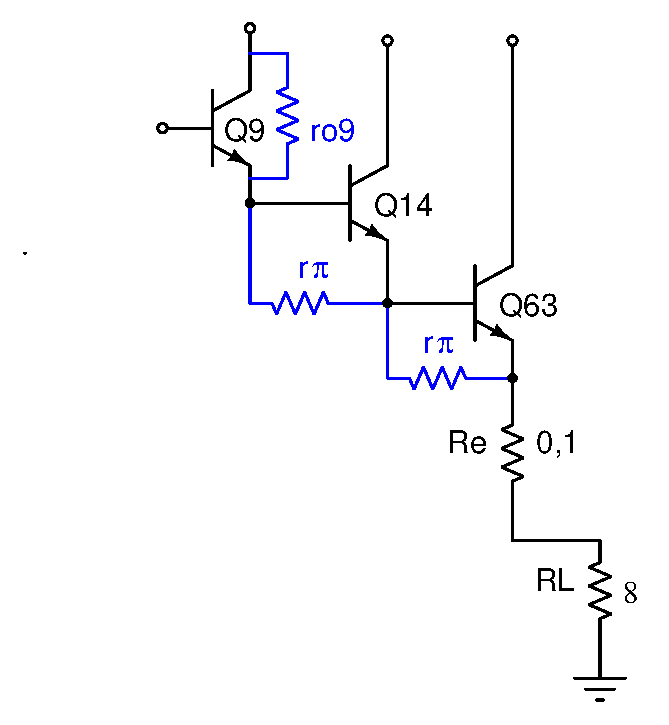
\includegraphics[scale=0.5]{ro.eps}
	 \caption{Diagrama para hallar la resistencia de salida del circuito sin realimentación.}
\end{figure}

\begin{itemize}
	\item Resistencia de salida sin realimentador: en esta situación se supone que, a los efectos de este cálculo, las resistencias de salida de los colectores comunes son iguales.
Entonces se calcula la resistencia de salida del circuito sin realimentar como
	\begin{equation}
		\centering
		R_o = \frac{1}{2} \cdot R_E + \frac{ r_{\pi}^{*} + r_{o,Q9} }{\beta^{*} } = \frac{1}{2} \left ( \SI{0.1}{\ohm} + \frac{\SI{32}{\kilo\ohm}}{75 \cdot 60} \right) = \SI{3.6}{\ohm}
	\end{equation}
	siendo
	\begin{equation}
		\centering
		r_{\pi}^{*} = 2 \cdot r_{\pi_{Q_{14}}} = 2 \cdot 60 \cdot \frac{25mV}{ \SI{110}{\milli\ampere}} = \SI{14}{\ohm} 
	\end{equation}
		
	%\begin{equation}
	%	\centering
	%	r_{o,Q9} = \frac{160V}{5mA} = \SI{32}{\kilo\ohm}
	%\end{equation}
		
	\item Resistencia de salida con realimentador
	\begin{equation}
		\centering
		R_{o,CR} = \frac{R_{o,SR}}{1+ af} = \frac{ \SI{3.6}{\ohm} }{1+1485} = \boxed{\SI{2.4}{\milli\ohm}} 
	\end{equation}
\end{itemize}


\subsection{Factor de amortiguamiento}

	En un sistema de audio, el factor de amortiguamiento es la relación entre la impedancia del altoparlante y la impedancia de salida del amplificador. Describe la capacidad del amplificador de controlar movimiento del altoparlante cuando se deja de excitarlo, en especial cercano a su frecuencia de resonancia. Este valor es de importancia en el contexto de las bajas frecuencias, o subwoofers, dado que la inercia de los diafragmas suele ser grande y el control de la suspensión débil, para permitir grandes excursiones.

\begin{equation}
	\centering
	f_a= \frac{Z_L}{Z_o} = \frac{ \SI{8}{\ohm}}{ \SI{2.4}{\milli\ohm}}= \boxed{\num{3333}}
	\label{ec:fa}
\end{equation}



\subsection{Resistencia de entrada}
	
	Con $R_{27}=\SI{22}{\kilo\ohm}$ el juego de resistores $R_{17}$ y $R_{18}$ deben sumar esa misma resistencia para compensar la tensión de corrimiento. Sin embargo, en un amplificador de audio se requiere que la impedancia de entrada sea alta. Se propone un \emph{bootstrap} entre los pines inversor y no-inversor para aumentar dicha resistencia, colocando $C_8$. Para evitar oscilasiones al unir dichas entradas se conecta $R_{20}$.
	

\begin{itemize}
	
	\HgraficarEPS{0.5}{ri}{Diagrama en bloque para hallar la resistencia de entrada.}{fig.esq_ri}
		
\item \textbf{Resistencia de entrada sin realimentación}
	
	\begin{equation}
		\centering
		R_{i,SR} = \SI{100}{\ohm} + R_{F1}//R_{F2} = \SI{100}{\ohm} + \SI{22}{\kilo\ohm}//\SI{1.1}{\kilo\ohm}
	\end{equation}
	
\item \textbf{Resistencia de entrada con realimentación}
	\HgraficarEPS{0.5}{ri_realim}{Diagrama en bloque para hallar la resistencia de entrada.}{fig.esq_ri_f}
	\begin{equation}
		\centering
		R_{i,CR} = (1+ af) \cdot R_{i,SR} = (1 + 1485) \cdot \SI{1.1}{\kilo\ohm} = \SI{1.6}{\mega\ohm}
	\end{equation}
	
\end{itemize}

Finalmente la resistencia que ve el generador es

$$ \SI{100}{\kilo\ohm}//\SI{1.6}{\mega\ohm} = \boxed{\SI{94}{\kilo\ohm}} $$





		\section{Fuentes conmutadas}
			La implementación de las fuentes de tensión de \SI{12}{\volt} y \SI{-12}{\volt} se realizó en base a los circuitos integrados \texttt{LM2576} y \texttt{LM2577}. Se propuso la construcción de dos circuitos independinetes, con el fin de no consumir toda la corriente de una sola fuente.

\subsection{Fuente reductora de tensión}
El diseño propuesto en la Figura \ref{fig.fte_12} corresponde a la configuración reductora de tensión cuya entrada es \SI{+30}{\volt}, y su salida \SI{+12}{\volt}. Debido a la dificultad de conseguir el modelo \textit{LM2565-12}, se decidió utilizar la versión ajustable, la cuál implica anexar dos resistencias de realimentación $R_2$ y $R_3$ según el esquema. El inductor $L_2$ y el capacitor $C_3$ permiten reducir el riple de la tensión de salida.


%\begin{figure}[H]
	%\centering
%	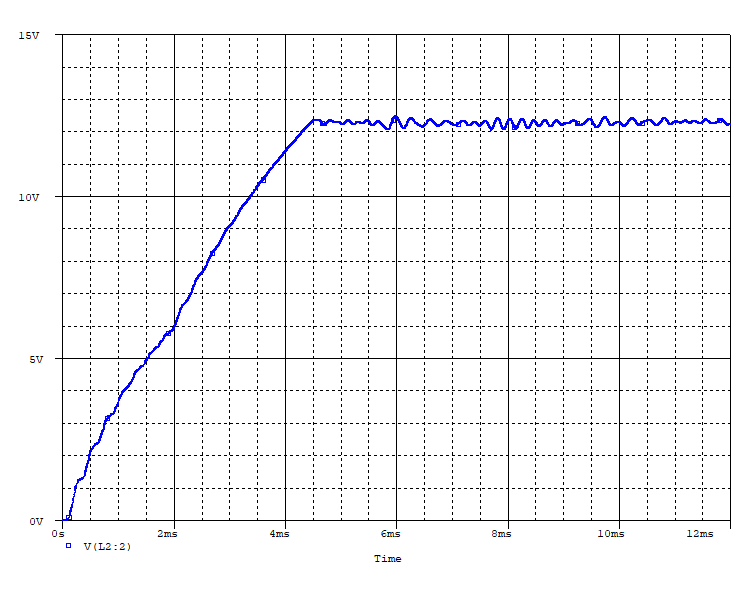
\includegraphics[angle=-90,width=1.1\textwidth, trim = 0.5cm 3.0cm 4cm 4cm]{fte_12_salida.png}
%	\caption{Salida de la fuente reductora de tensión.}
%	\label{fig.fte_salida_12}
%\end{figure}


\begin{figure}
	\centering
	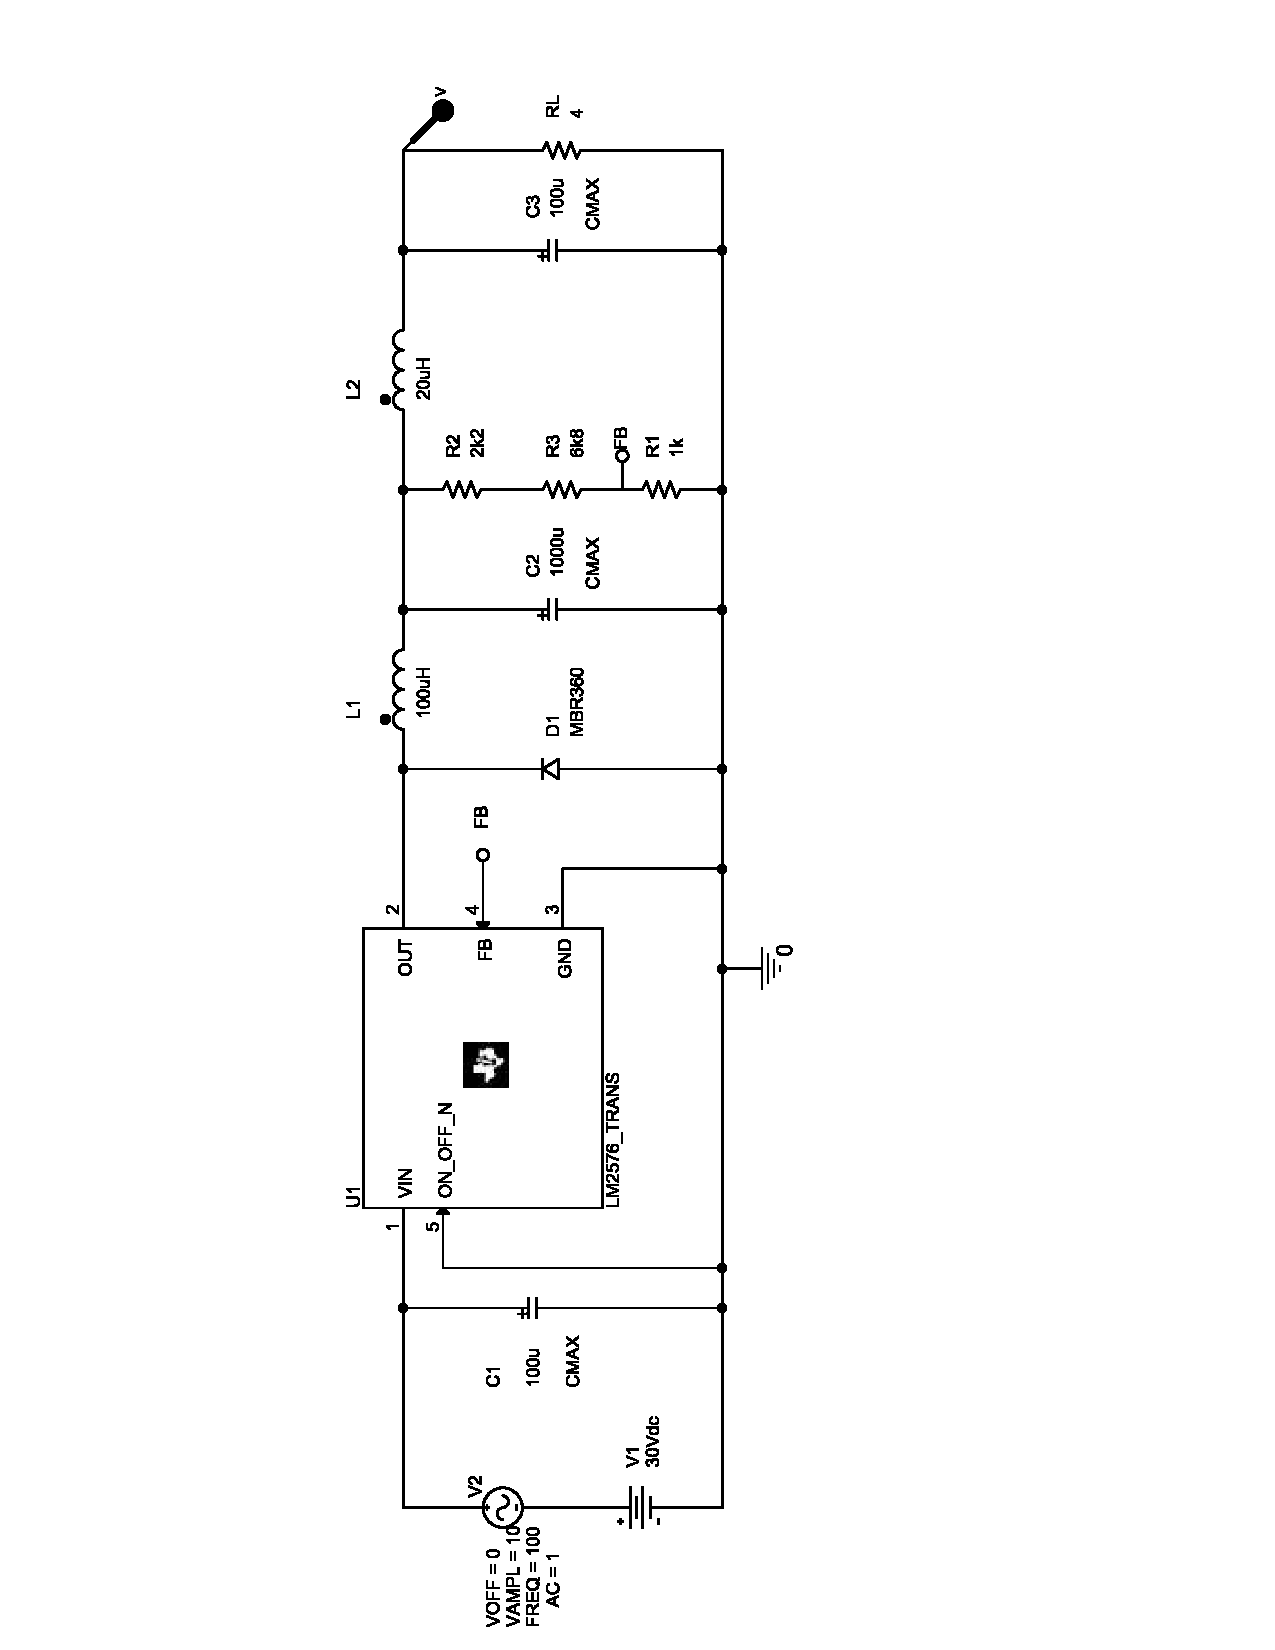
\includegraphics[width=0.4\textwidth, angle=-90, trim= 4.0cm 3cm 7cm 4cm]{fte_12_esquema.pdf}
	\caption{Fuente reductora de tensión.}
	\label{fig.fte_12}
\end{figure}


Debido a que la fuente de entrada puede variar en un 20\%, en la simulación se anexó una fuente alterna en serie para analizar el comportamiento de la salida ante alteraciones de $V_E$. La salida resultante se muetra en la Figura \ref{fig.fte_salida_12}, observándose una variación del orden de decenas de $\SI{}{\milli\volt}$.



\HgraficarPNG{0.5}{fte_12_salida}{Salida de la fuente reductora de tensión}{fig.fte_salida_12}


\subsection{Fuente elevadora de tensión}

Para el circuito elevador, desde \SI{-30}{\volt} a \SI{-12}{\volt}, se propuso el diseño de la Figura \ref{fig.fte_elevadora}. 
No se logró realizar la simulación debido a la inexistencia del modelo de \texttt{LM2577} en \emph{PSpice}. 
La elección de los componentes se detalla en la nota de aplicación, aunque sus valores podrán variar empíricamente.

\begin{figure}[H]
	\centering
	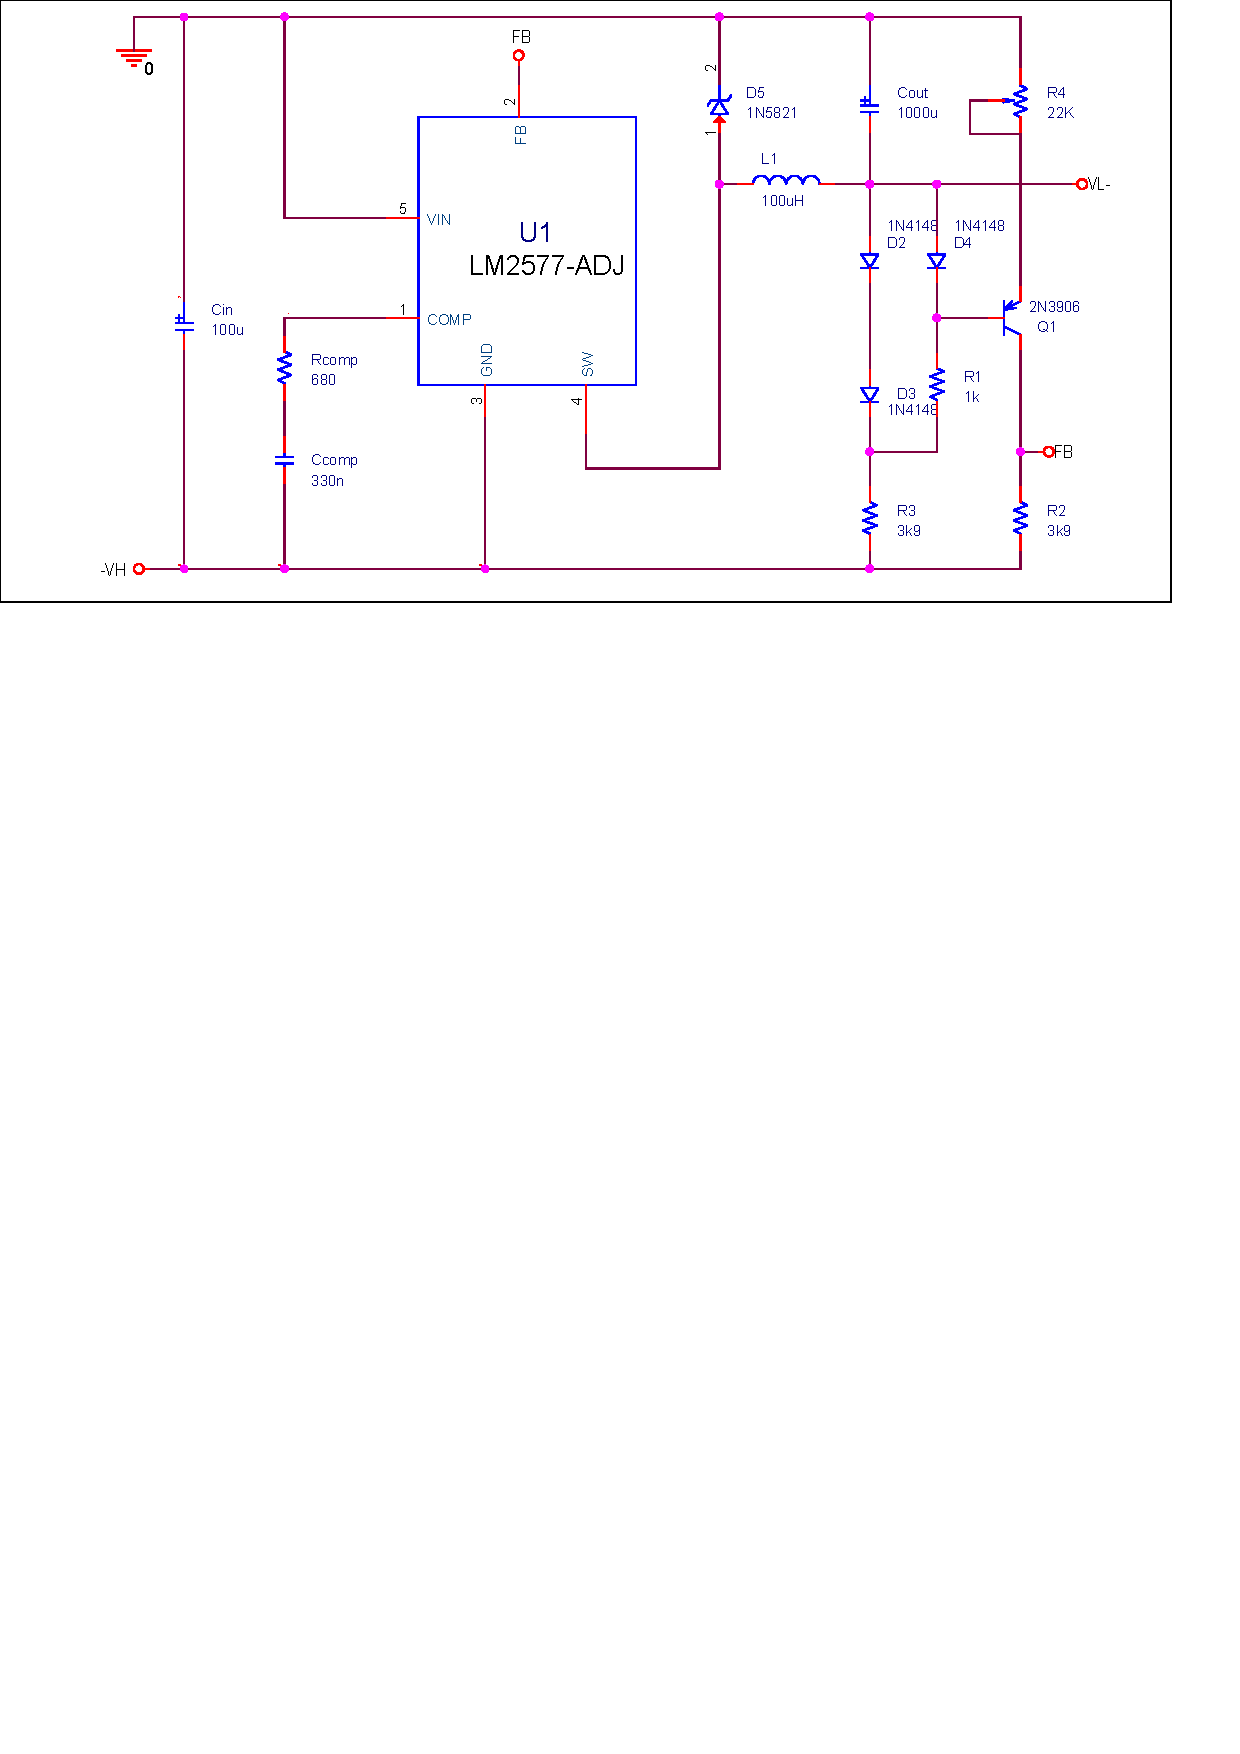
\includegraphics[width=0.6\textwidth, trim = 0cm 19cm 2cm 0cm]{lm2577}
	\caption{Fuente elevadora de tensión.}
	\label{fig.fte_elevadora}
\end{figure}



%		\section{Características del amplificador}
%				\Juan{Borrar y redirigir}
\subsection{Resistencia de entrada}

\begin{itemize}
	
	\HgraficarEPS{0.5}{ri}{Diagrama en bloque para hallar la resistencia de entrada.}{fig.esq_ri}
		
\item \textbf{Resistencia de entrada sin realimentación}
	
	\begin{equation}
		\centering
		R_{i,SR} = \SI{100}{\ohm} + R_{F1}//R_{F2} = \SI{100}{\ohm} + \SI{22}{\kilo\ohm}//\SI{1.1}{\kilo\ohm}
	\end{equation}
	
\item \textbf{Resistencia de entrada con realimentación}
	\HgraficarEPS{0.5}{ri_realim}{Diagrama en bloque para hallar la resistencia de entrada.}{fig.esq_ri_f}
	\begin{equation}
		\centering
		R_{i,CR} = (1+ af) \cdot R_{i,SR} = (1 + 1485) \cdot \SI{1.1}{\kilo\ohm} = \SI{1.6}{\mega\ohm}
	\end{equation}
	
\end{itemize}

Finalmente la resistencia que ve el generador es

$$ \SI{100}{\kilo\ohm}//\SI{1.6}{\mega\ohm} = \boxed{\SI{94}{\kilo\ohm}} $$


\subsection{Impedancia de salida}

\begin{figure}[H]
	 \centering
	 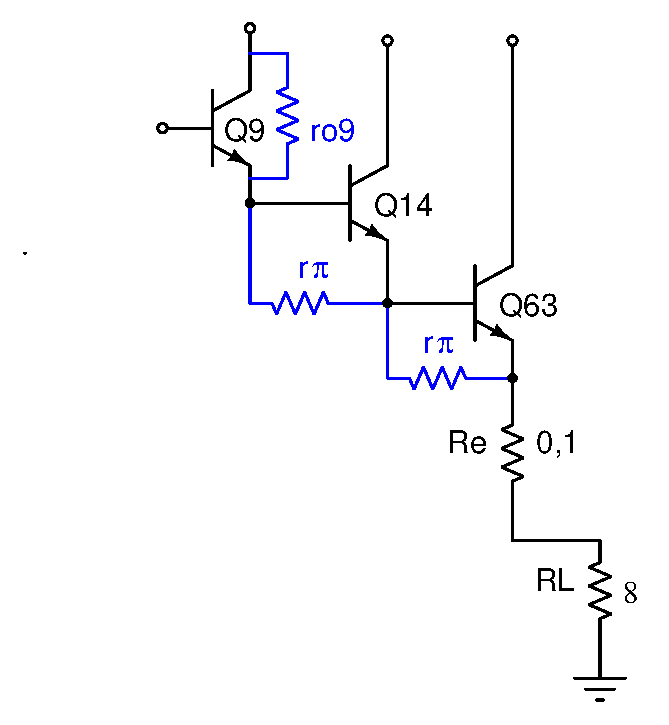
\includegraphics[scale=0.5]{ro.eps}
	 \caption{Diagrama para hallar la resistencia de salida del circuito sin realimentación.}
\end{figure}

\begin{itemize}
	\item Resistencia de salida sin realimentador: en esta situación se supone que, a los efectos de este cálculo, las resistencias de salida de los colectores comunes son iguales.
Entonces se calcula la resistencia de salida del circuito sin realimentar como
	\begin{equation}
		\centering
		R_o = \frac{1}{2} \cdot R_E + \frac{ r_{\pi}^{*} + r_{o,Q9} }{\beta^{*} } = \frac{1}{2} \left ( \SI{0.1}{\ohm} + \frac{\SI{32}{\kilo\ohm}}{75 \cdot 60} \right) = \SI{3.6}{\ohm}
	\end{equation}
	siendo
	\begin{equation}
		\centering
		r_{\pi}^{*} = 2 \cdot r_{\pi_{Q_{14}}} = 2 \cdot 60 \cdot \frac{25mV}{ \SI{110}{\milli\ampere}} = \SI{14}{\ohm} 
	\end{equation}
		
	%\begin{equation}
	%	\centering
	%	r_{o,Q9} = \frac{160V}{5mA} = \SI{32}{\kilo\ohm}
	%\end{equation}
		
	\item Resistencia de salida con realimentador
	\begin{equation}
		\centering
		R_{o,CR} = \frac{R_{o,SR}}{1+ af} = \frac{ \SI{3.6}{\ohm} }{1+1485} = \boxed{\SI{2.4}{\milli\ohm}} 
	\end{equation}
\end{itemize}

\subsection{Factor de amortiguamiento}

En un sistema de audio, el factor de amortiguamiento es la relación entre la impedancia del altoparlante y la impedancia de salida del amplificador. Describe la capacidad del amplificador de controlar movimiento del altoparlante cuando se deja de excitarlo, en especial cercano a su frecuencia de resonancia. Este valor es de importancia en el contexto de las bajas frecuencias, o subwoofers, dado que la inercia de los diafragmas suele ser grande y el control de la suspensión débil, para permitir grandes excursiones.

\begin{equation}
	\centering
	f_a= \frac{Z_L}{Z_o} = \frac{ \SI{8}{\ohm}}{ \SI{2.4}{\milli\ohm}}= \boxed{\num{3333}}
	\label{ec:fa}
\end{equation}




						
%		\section{Polarización}\label{sec:pol}
%			\input{III1_polarizacion.tex}
%		
%		\section{Ganancia de lazo}\label{sec:gan_lazo}
%			\input{III2_gan_lazo.tex}
%		
%		\section{Ganancia global}\label{sec:gan_global}
%			\input{I3_gan_global.tex}
%	
%		\section{Máxima potencia sobre la carga}\label{sec:pot_carga}
%			\input{I4_pot_carga.tex}
%	
%		\section{Impedancia de entrada}\label{sec:zi}
%			\input{I5_zi.tex}
%	
%		\section{Impedancia de salida}\label{sec:zo}
%			\input{I6_zo.tex}
%		
%		\section{Factor de amortiguamiento}\label{sec:amort}
%			\input{I7_amortiguamiento.tex}
%	
%		\section{Máxima tensión pico sobre la carga}\label{sec:pico_carga}
%			\input{I8_pico_carga.tex}
%		\pagebreak	
%		\section{Máxima eficiencia del amplificador}\label{sec:eficiencia}
%			\input{I9_eficiencia.tex}
%		\pagebreak	
%		\section{Disipadores}\label{sec:disipadores}
%			\input{I10_disipadores.tex}
%	\pagebreak
	\part{Diseño del circuito impreso - \emph{PCB}}\label{part:pcb}

		\section{Elección de componentes}\label{sec:componentes}
			En las Tablas \ref{tab:lst_tr}, \ref{tab:lst_cap} y \ref{tab:lst_resist} se detallan todos los componentes necesarios para la implementación del circuito, teniendo en cuenta los valores comerciales disponibles.

\begin{table}[h!]
	\centering
	\begin{tabular}{cccc}
		\toprule
		Código & Nombre & Características & Cantidad \\
		\midrule
		\texttt{2SC5198} & Q62, Q63 & NPN & 2 \\
		\texttt{2SA194} & Q64, Q65 & PNP & 2 \\ 
		\texttt{MJE340} & Q14, Q16, Q26 & NPN & 3 \\
		\texttt{MJE350} & Q15, Q17 & PNP & 2 \\
		\texttt{MPSA56} & Q1, Q8, Q9, Q12, Q13, Q27, Q28& PNP   & 7 \\ 
		\texttt{MPSA06} & Q30, Q29, Q43, Q20 & NPN  & 4 \\
		\texttt{BC817}  & Q56, Q59, Q61, Q60 & NPN SMD & 4 \\
		\texttt{BC807}  & Q54, Q55, Q56, Q57 & PNP SMD & 4 \\
		\texttt{BC847}  & Q52 & NPN SMD & 1  \\
		\texttt{BC857}  & Q53 & PNP SMD & 1 \\
		\midrule
		\texttt{1N4148} & D1,2,3,4,14,15,18,19,20,21  & Diodo de alta conmutación & 10 \\
		\texttt{MBRB1645T4G} & D16, D17 & Diodo Schottky & 2 \\
		\bottomrule
	\end{tabular}
	\caption{Transistores y diodos utilizados en el circuito.}
	\label{tab:lst_tr}
\end{table}

\begin{table}[h!]
	\centering
	\begin{tabular}{cccc}
		\toprule
		Valor & Nombre & Tecnología & Cantidad \\
		\midrule
		\SI{10}{\micro\farad} & C18 & Electrolítico & 1 \\	 
		\SI{47}{\micro\farad} & C1, C4, C20, & Electrolítico & 3 \\
		\SI{1}{\milli\farad} & C11 & Electrolítico & 1 \\
		\SI{100}{\nano\farad} & C2, C9, C12, C15 & Poliéster & 3 \\
		\SI{1}{\nano\farad} & C7 & Poliéster & 1 \\
		\SI{330}{\pico\farad} & C10 & Cerámico & 1 \\
		\bottomrule
	\end{tabular}
	\caption{Capacitores y tecnología de los mismos para la implementación del circuito.}
	\label{tab:lst_cap}
\end{table}

\begin{table}[h!]
	\centering
	\begin{tabular}{cccc}
		\toprule
		Valor & Nombre & Tecnología & Cantidad \\
		\midrule
		\SI{0.1}{\ohm} & R32, R33 & Alambre, 5W & 2 \\
		\SI{10}{\ohm} & R39 & Alambre, 5W & 1 \\		
		\SI{10}{\ohm} & R38 & Metalfilm 1W & 1 \\
		\SI{100}{\ohm} & R28, R29, R35, R36 & Metalfilm 1W & 4 \\
		\SI{22}{\kilo\ohm} & R27 & Metalfilm, 1W & 1 \\
		\SI{10}{\ohm} & R16, R23 & SMD 0805 & 2 \\
		\SI{15}{\ohm} & R42 & SMD 0805 & 1 \\
		\SI{56}{\ohm} & R49, R50, R53, R54 & SMD 0805 & 4 \\
		\SI{68}{\ohm} & R21, R25 & SMD 0805 & 2 \\
		\SI{100}{\ohm} & R1,13,14,20,76 & SMD 0805 & 5 \\
		\SI{270}{\ohm} & R59, R60 & SMD 0805 & 2 \\ 
		\SI{560}{\ohm} & R51, R62 & SMD 0805 & 2 \\
		\SI{680}{\ohm} & R44 & SMD 0805 & 1\\
		\SI{1}{\kilo\ohm} & R73, R74, R15, R62, R63, R67, R68  & SMD 0805 & 7 \\
		\SI{2.2}{\kilo\ohm} & R5, R47 & SMD 0805 & 2 \\ 
		\SI{3.3}{\kilo\ohm} & R43 & SMD 0805 & 1 \\
		\SI{5.6}{\kilo\ohm} & R61, R66 & SMD 0805 & 2 \\
		\SI{8.2}{\kilo\ohm} & R64, R65 & SMD 0805 & 2 \\
		\SI{10}{\kilo\ohm} & R17, R18 & SMD 0805 & 2 \\
		\SI{100}{\kilo\ohm} & R19 & SMD 0805 & 2 \\
		\bottomrule
	\end{tabular}
	\caption{Lista de resistencias requeridas para el circuito.}
	\label{tab:lst_resist}
\end{table}


		\section{Criterios de Ruteo}\label{sec:ruteo}
			\begin{itemize}
	\item Las fuentes de alimentación se se colocaron lo más cerca posible de la etapa de salida, ya ésta es la que maś corriente consume.
	\item Sabiendo que la corriente máxima que puede circular por la salida es de \SI{3.5}{\ampere}, una pista de 75 mills resulta sufifiente para las pistas de potencia.
	\Flor{Completar}
	\item Pistas de baja potencia de mills.
	\item El camino entre la salida y realimentación se colocó lo más cerca posible, lo mismo entre el el comparador y la salida, debido a que se reuiere velocidad. 
	\item No se dejaron espacios vacíos, sino que se dejaron con cobre y conectados a tierra para así obtener islas de masa.
	\item Los transistores de entrada se colocaron lo más cercanos posible para obtener un buen acoplamiento térmico.
	\item Se verificó que no se formen espiras, ya que se comportarían como inductancias.
	\item Se procuró que las pistas no posean esquinas con puntas ó ángulos agudos para evitar interferencias y facilitar la fabricación.

\end{itemize}


		\pagebreak
		\section{Circuito Impreso}
			Una vez elegidos los componentes y teniendo en cuenta los criterios de ruteo ya descriptos, se procedió al diseñó el circuito impreso mediante \textit{Orcad}. El primer paso es asignarle a cada componente su corrospondiente \textit{footprint}, los cuales deben ser elegidos cuidadosamente y verificados por la hoja de datos. El diseño del circuito impreso se muestra en las figuras \ref{fig.top} y \ref{fig.bottom}. 


\HgraficarPNG{0.5}{top_color}{Diseño de PCB}{fig.pcb_top}
\HgraficarPNG{0.5}{bottom_color}{Diseño de PCB}{fig.pcb_bottom}

%	\pagebreak
	\part{Análisis por simulación}\label{part:sim}
		
		\section{Polarización}\label{sec:sim_pol}
			Con el fin de corroborar y ajustar los resultados teóricos obtenidos, se realiza la simulación del circuito mediante \texttt{SPICE Orcad}.

\begin{figure}[H]
	\centering
	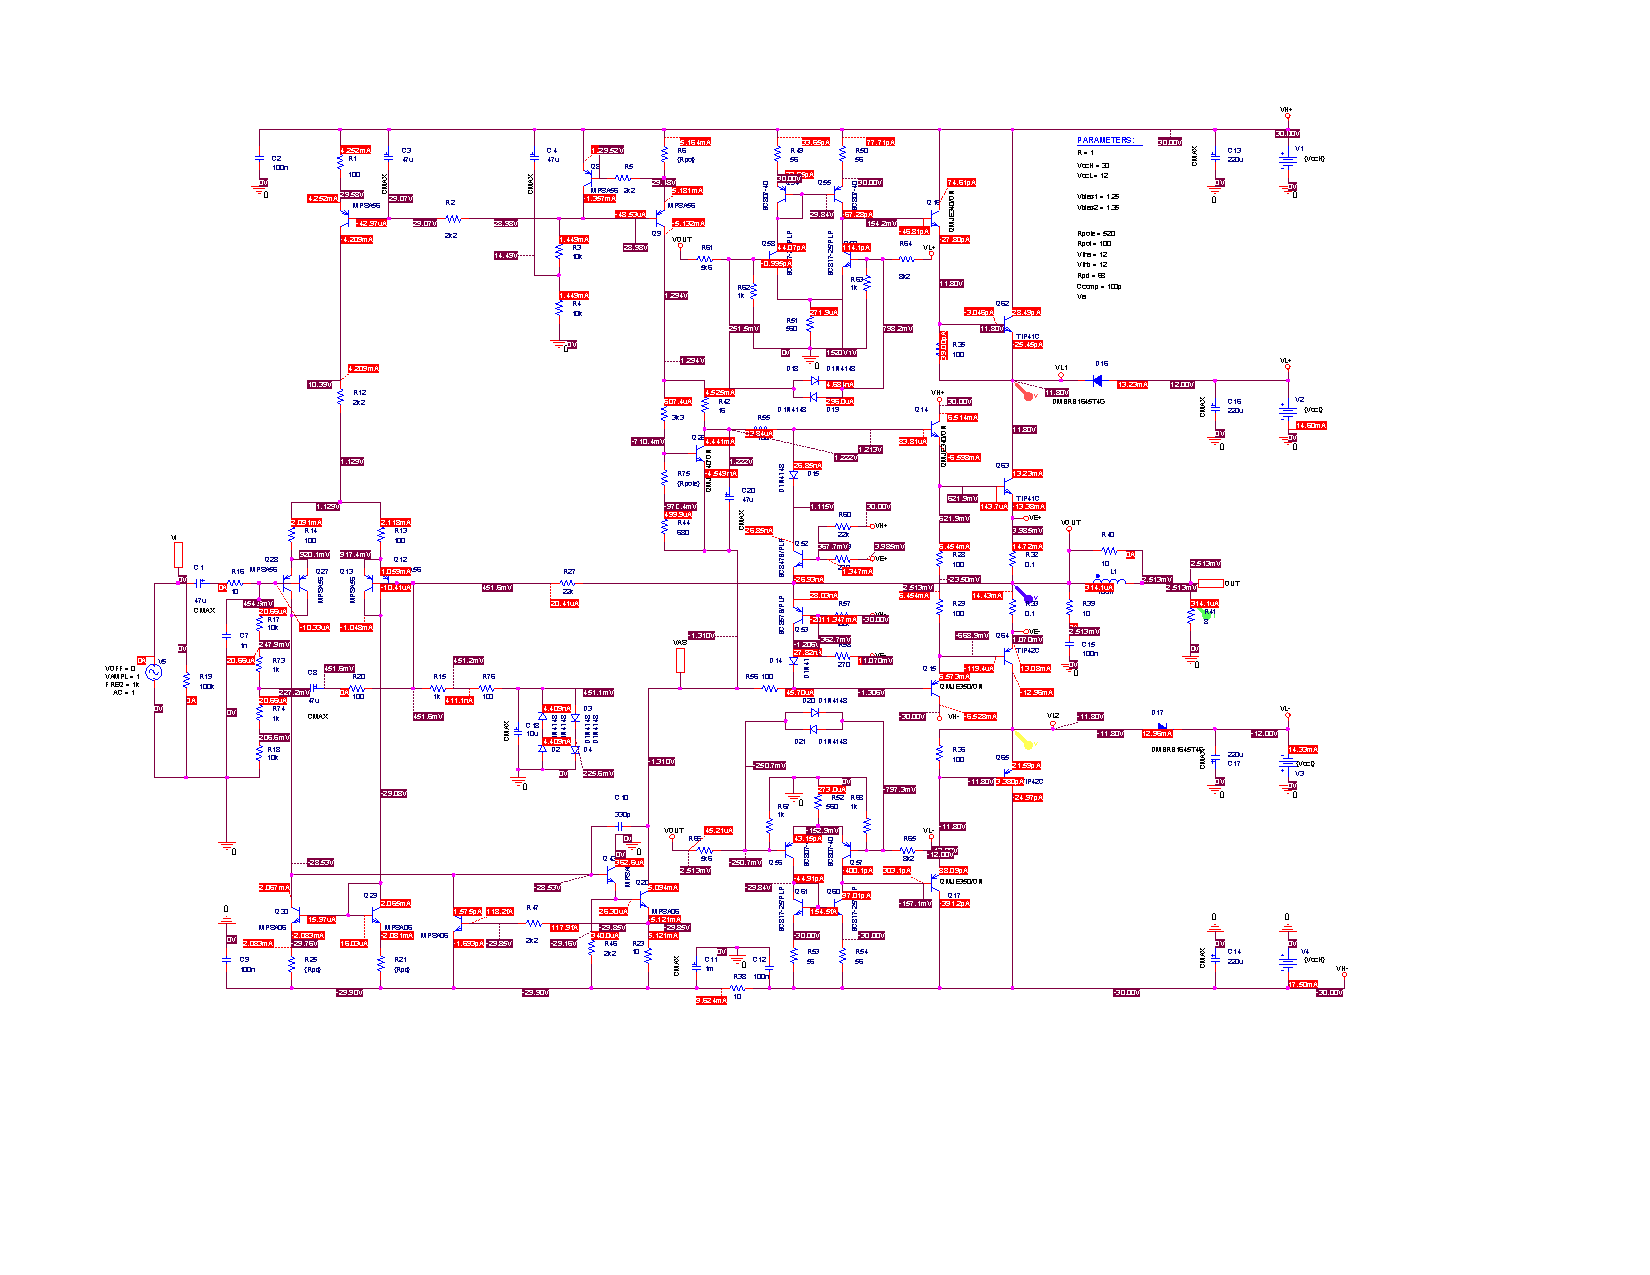
\includegraphics[width=1.2\textwidth, trim = 4cm 4cm 4cm 2cm]{sim_polarizacion.pdf}
	\caption{Tensiones y corrientes de reposo.}
	\label{fig:sim_pol}
\end{figure}


En la Figura \ref{fig:sim_pol} se muestran las tensiones y corrientes en continua, siendo coherentes con los valores esperados.


		
		\section{Compensación}\label{sec:sim_compensacion}
			Para hallar el valor del capacitor de compensación (presente entre la base y colector del transistor de VAS), se impone una señal cuadrada en la entrada y se observa como resulta la salida. Se realizó una simulación al variar el valor de la capacidad desde \SI{100}{\pico\farad} (curva naranja) hasta \SI{400}{\pico\farad} (curva celeste) de a \SI{100}{\pico\farad}. El resultado se muestra en la figura \ref{fig:var_cap}


\HgraficarPNG{0.5}{sim_var_cap_compensacion.png}{Variación de la capacitancia de compensación.}{fig:var_cap}

Por lo tanto para que el circuito esté compensado se eligió un valor comercial de \SI{330}{\pico\farad}.

		\section{Impedancia de entrada}{\label{sec:sim_zi}
			\HgraficarPNG{0.5}{sim_rin.png}{Impedancia de entrada}{fig.sim_rin}


Para analizar el comportamiento de la impedancia de entrada en función de la frecuencia, se colocó una fuente \texttt{AC} en serie con una resistencia de prueba y se midió la corriente que pasa por ella y la tensión en el nodo de entrada. Al realizar la división, se obtuvo la Figura \ref{fig.sim_ri}. Se puede observar que para frecuencias medias, la resistencia resultó ser aproximadamente \SI{91}{\kilo\ohm}, valor próximo al hallado analíticamente ($R_{if}=\SI{100}{\kilo\ohm}$).


		\section{Impedancia de salida}\label{sec:sim_zo}
			\HgraficarPNG{0.5}{sim_rout.png}{Impedancia de salida en función de la frecuencia.}{fig.sim_ro}

Para realizar la simulación de la impedancia de salida, se pasivó la señal de entrada y se colocó una fuente alterna de prueba en el nodo de salida junto con una resistencia de prueba de \SI{0.1}{\ohm} y un capacitor de \SI{10}{\micro\farad} en serie. Mediante un análisis \texttt{AC} se midió la tensión de salida y la corriente en la resistencia de prueba, y al realizar la división se obtiene la impedancia buscada. El resultado obtenido se muestra en la figura \ref{fig.sim_ro}. Se puede observar que para frecuencias bajas y medias, hasta aproximadamente \SI{10}{\kilo\hertz}, la resistencia de salida es muy pequeña, del orden de los \SI{}{\milli\ohm}. Luego, a partir de \SI{10}{\kilo\hertz} comienza a incrementarse siendo el valor máximo \SI{6.5}{\ohm}.


		\section{Respuesta en frecuencia}\label{sec:sim_rta_frec}
			\begin{figure}[H]	
	\centering
	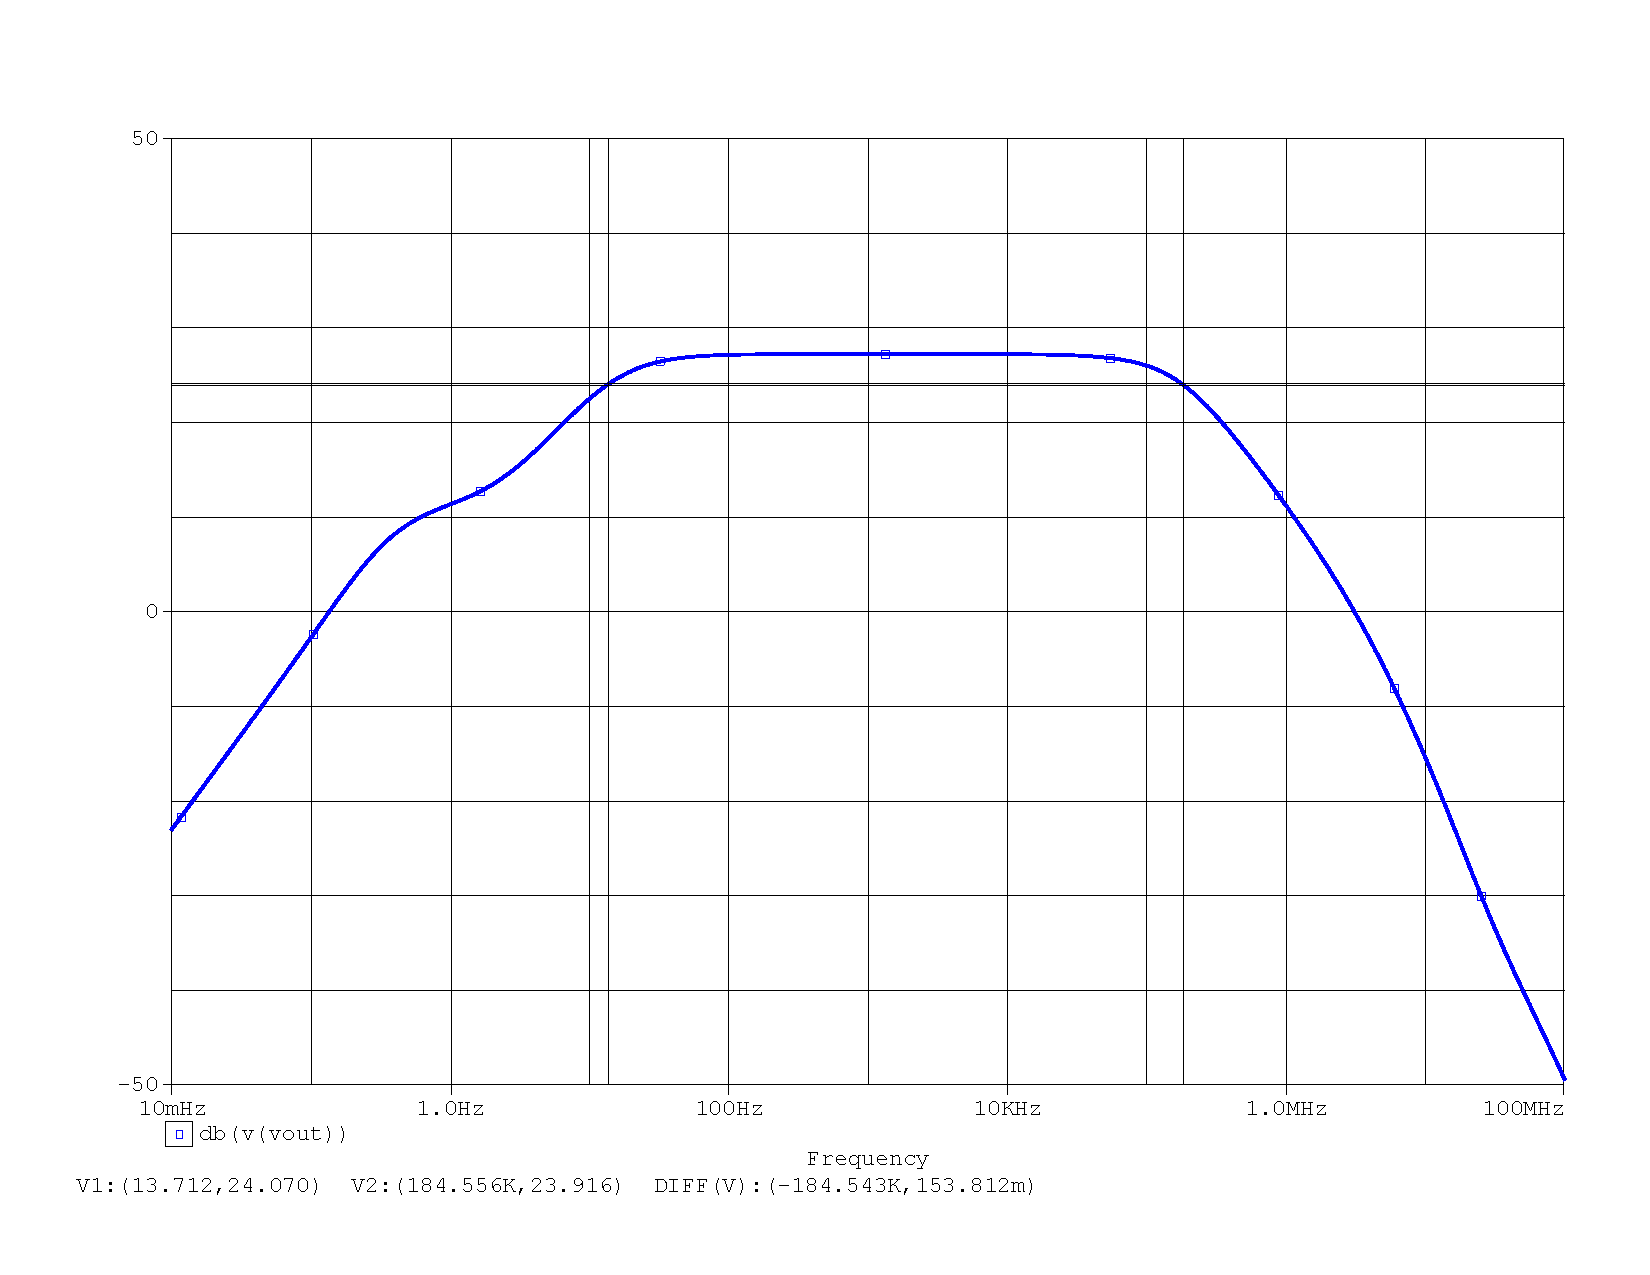
\includegraphics[scale=0.5]{sim_rta_frec_completo.pdf}
	\caption{Respuesta en frecuencia del circuito completo.}
	\label{fig:rta_frec}
\end{figure}

\begin{align}
	\centering
	f_{L} & = \SI{14}{\hertz}\\
	f_H & = \SI{185}{\kilo\hertz}
\end{align}


		\section{Ancho de banda de potencia}\label{sec:sim_bw}
			%\begin{figure}[H]
%	\centering
%	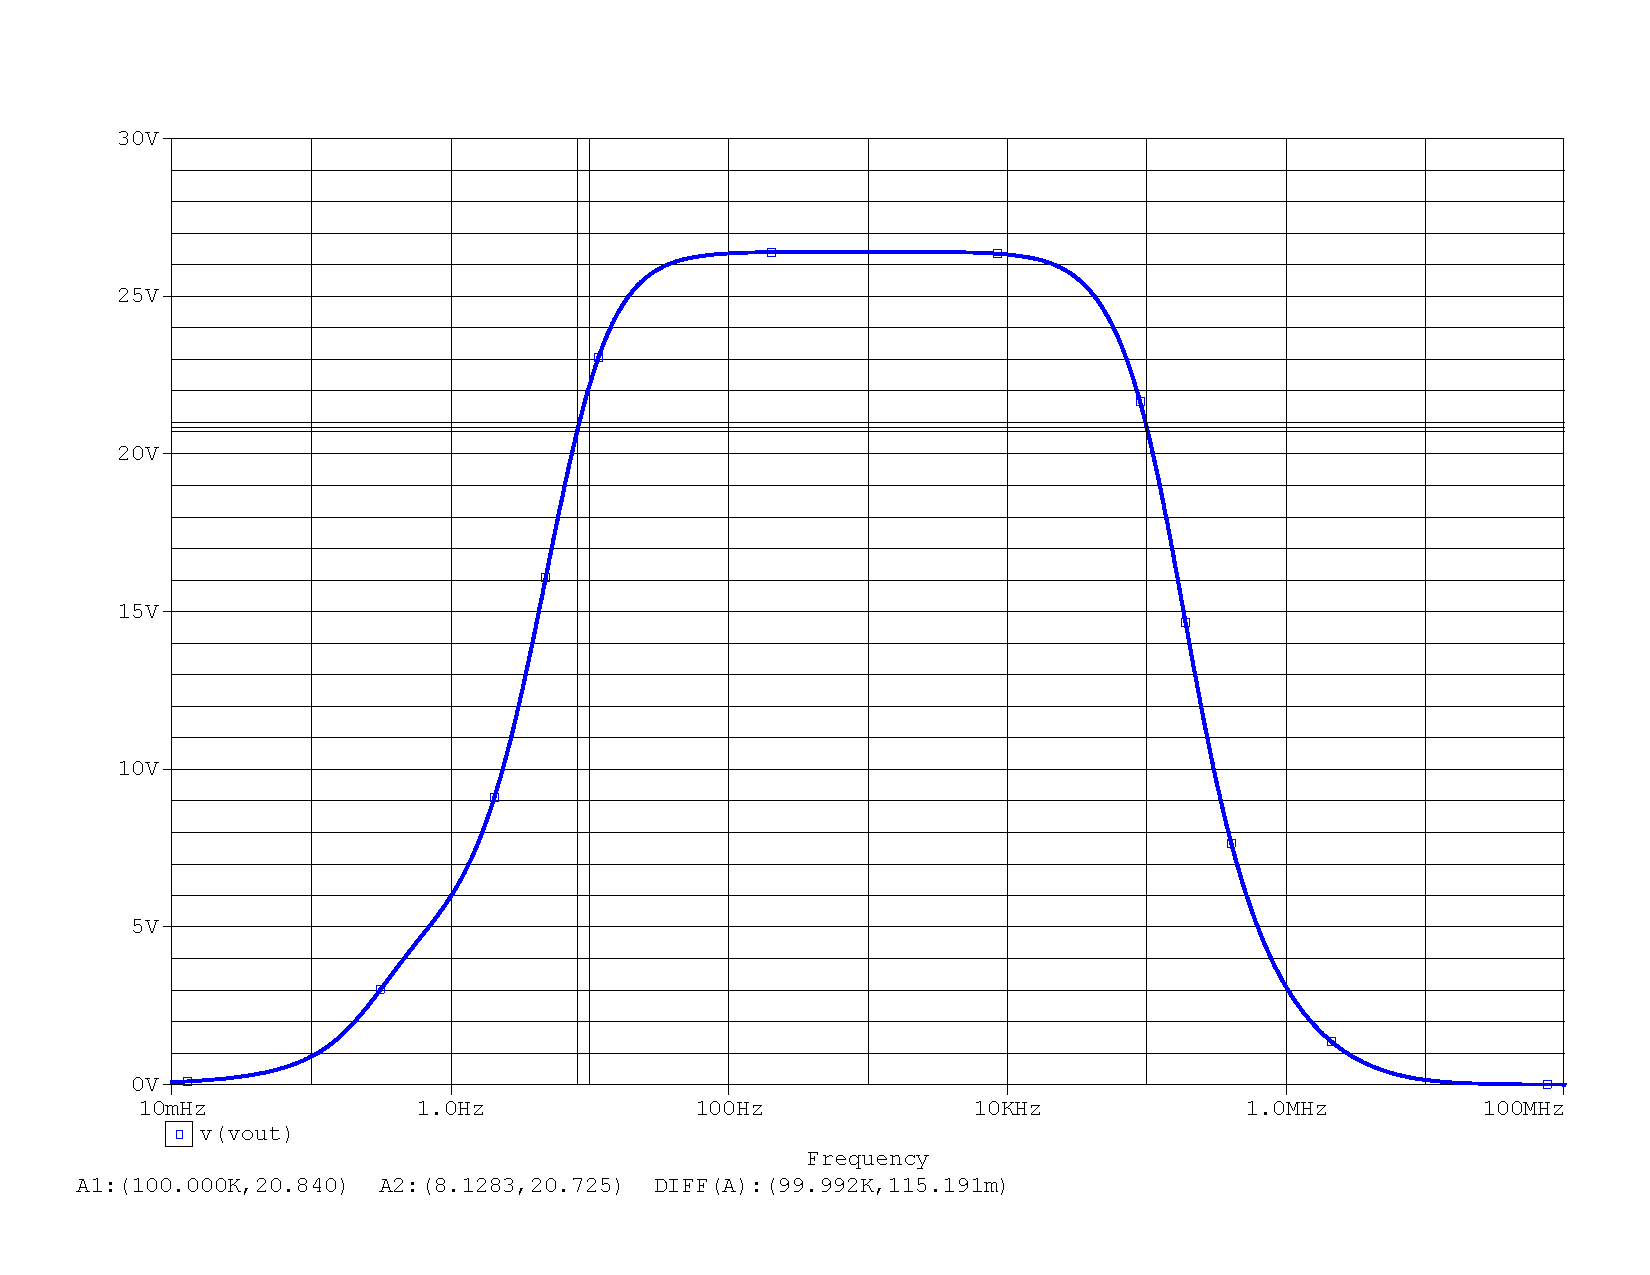
\includegraphics[scale=0.5]{sim_bw_potencia.pdf}
%	\caption{Ancho de banda de potencia}
%	\label{fig:sim_bw}
%\end{figure}

\HgraficarPNG{0.5}{sim_rta_max_potencia.png}{Ancho de banda de potencia}{fig:sim_bw}

El ancho de banda de potencia indica la máxima frecuencia para la cuál el amplificador logra reproducir una señal sinusoidal a máxima potencia. Para este caso, la máxima tensión sin distorsión apreciable es aproximadamente \SI{26}{\volt}. A partir de la Figura \ref{fig:sim_bw} se obtiene

\begin{align}
	\centering
	f_L &= \SI{14}{\hertz} \\
	f_H &= \SI{160}{\kilo\hertz}
\end{align}


		\section{Respuesta al escalón}\label{sec:sim_escalon}
			\subsubsection{Respuesta la escalón para pequeña señal}

\Flor{El escalón de salida quedó con un offset, esto pasó por cambiar el cap de 1m por el de 10u, pero era necesario para determinar la fl.}

\HgraficarPNG{0.5}{sim_rta_escalon_peque.png}{Respuesta al escalón en pequeña señal.}{fig:rta_escalon_peque}

%\begin{figure}[H]
%	\centering
%	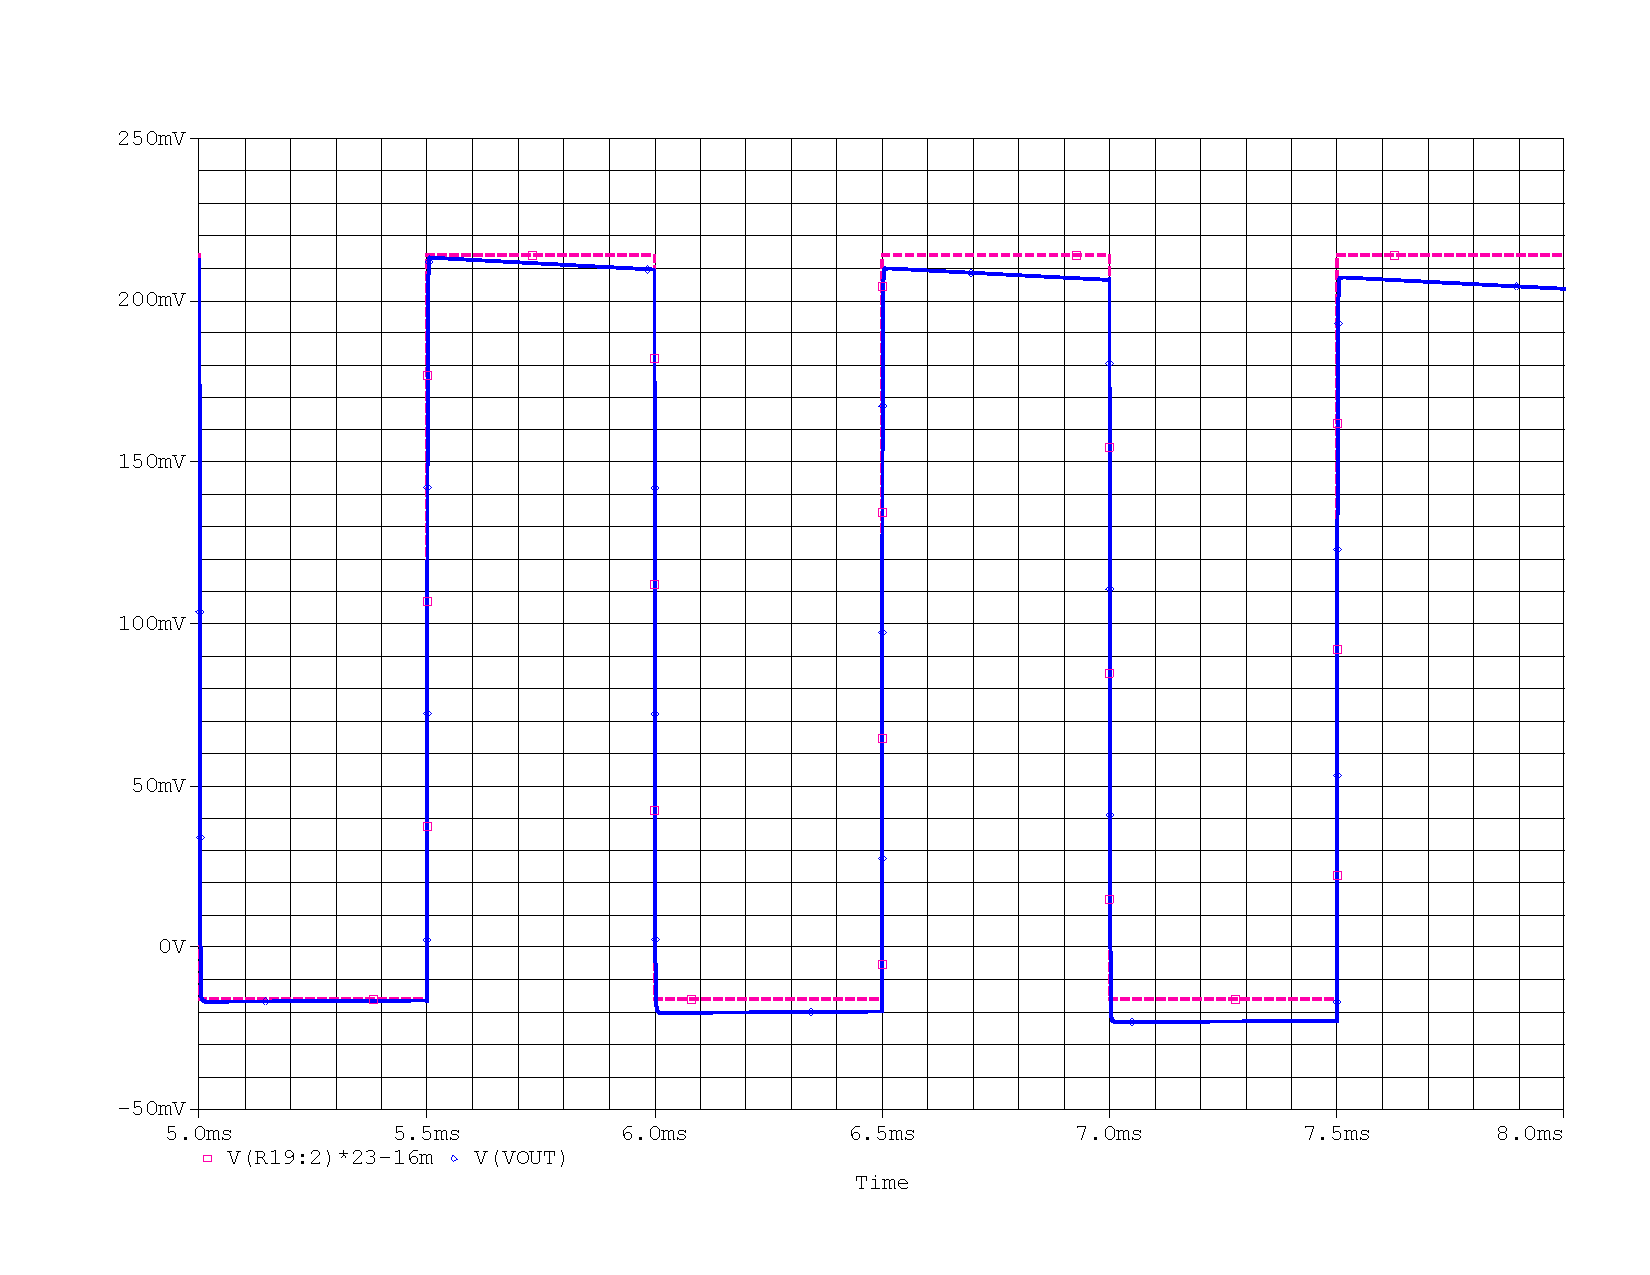
\includegraphics[scale=0.4]{sim_rta_escalon_senial_peque.pdf}
%	\caption{Respuesta al escalón en pequeña señal.}
%	\label{fig:rta_escalon_peque}
%\end{figure}

\subsubsection{Respuesta al escalón para gran señal}

\HgraficarPNG{0.5}{sim_rta_escalon_gran.png}{Respuesta al escalón en gran señal.}{fig:rta_escalon_gran}

%\begin{figure}[H]
%	\centering
%	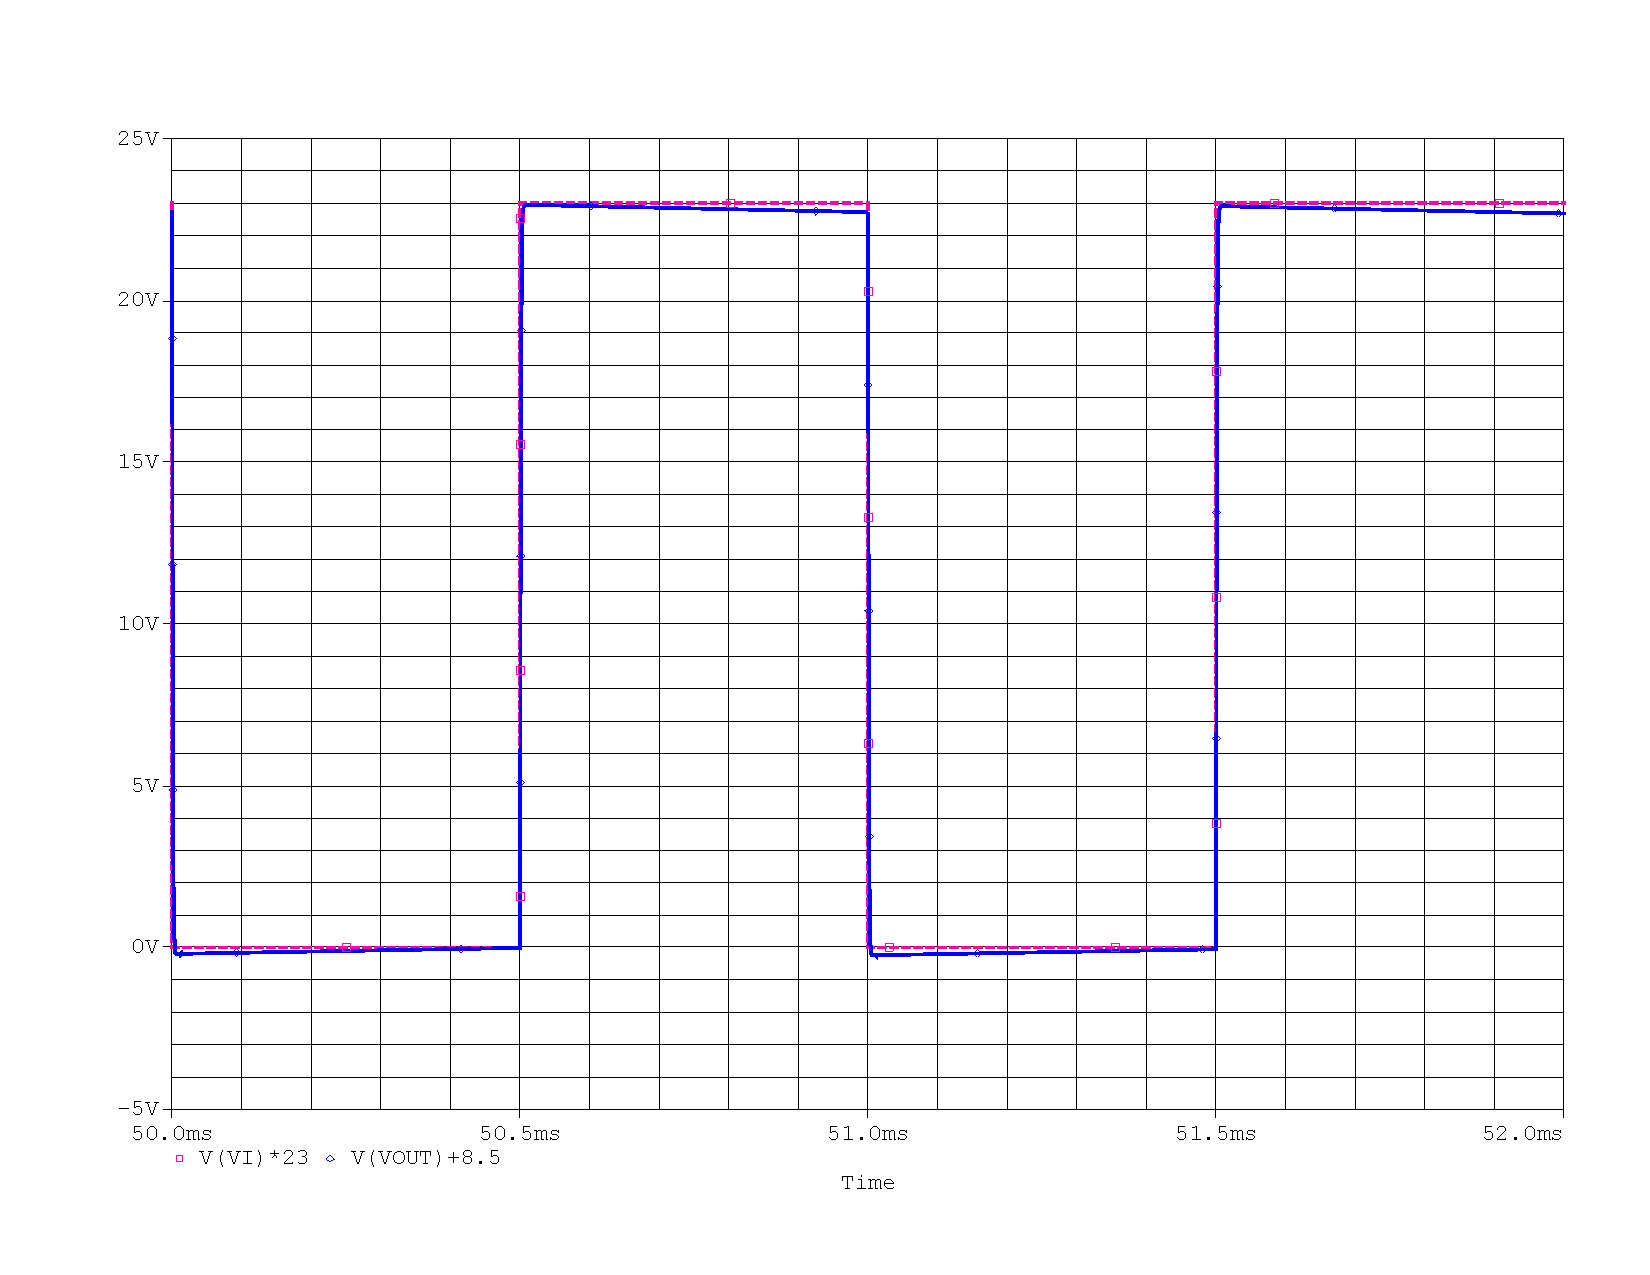
\includegraphics[scale=0.4]{sim_rta_escalon_gran_senial.pdf}
	%\caption{Respuesta al escalón en gran señal.}
	%\label{fig:rta_escalon_gran}
%\end{figure}

\subsubsection{Ancho de banda}

	Este parámetro se obtiene a partir de la simulación de la respuesta al escalón del circuito en pequeña señal (\SI{10}{\milli\volt}).
	
	\HgraficarPNG{0.5}{sim_rta_escalon_gran_zoom.png}{Respuesta al escalón en pequeña señal.}{fig:rta_escalon_peque}

%\begin{figure}[H]
%	\centering
%	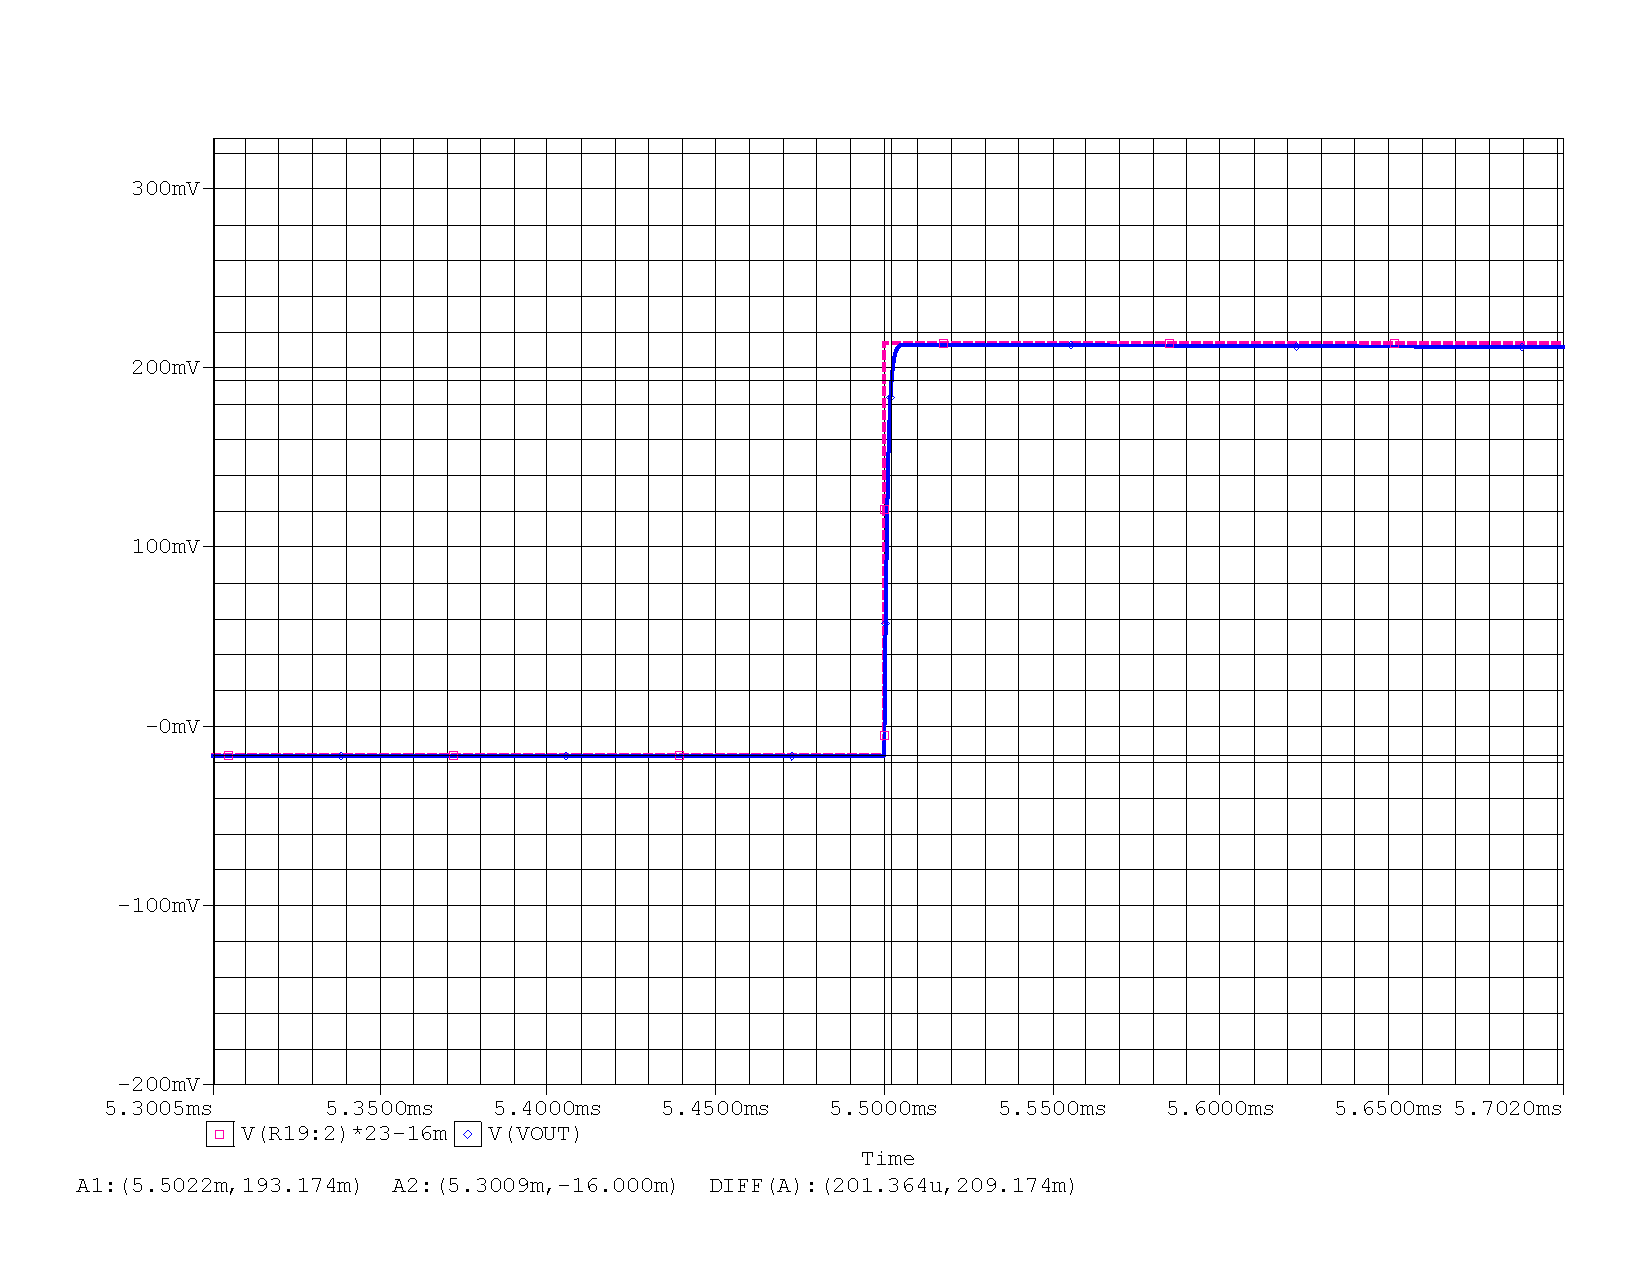
\includegraphics[scale=0.4]{sim_rta_escalon_senial_peque_zoom.pdf}
% 	\caption{Respuesta al escalón en pequeña señal.}
%	\label{fig:rta_escalon_peque}
%\end{figure}

	Observando la figura \ref{fig:sim_bw} el tiempo de crecimiento ($\tau_r$), se puede determinar el ancho de banda mediante la ecuación \eqref{ec:bw}.

	\begin{equation}
		\centering
		\mathrm{BW} = \frac{\num{0,35}}{\tau_r} = \frac{0,35}{\SI{2}{\micro\second}} = \boxed{\SI{175}{\kilo\hertz}}
		\label{ec:bw}
	\end{equation}

\subsubsection{\textit{Slew Rate}}

\HgraficarPNG{0.5}{sim_rta_escalon_gran_zoom.png}{Respuesta al escalón en gran señal ampliado.}{fig:sim_rta_escalon_gran_sr}

%\begin{figure}[H]
%	\centering
%	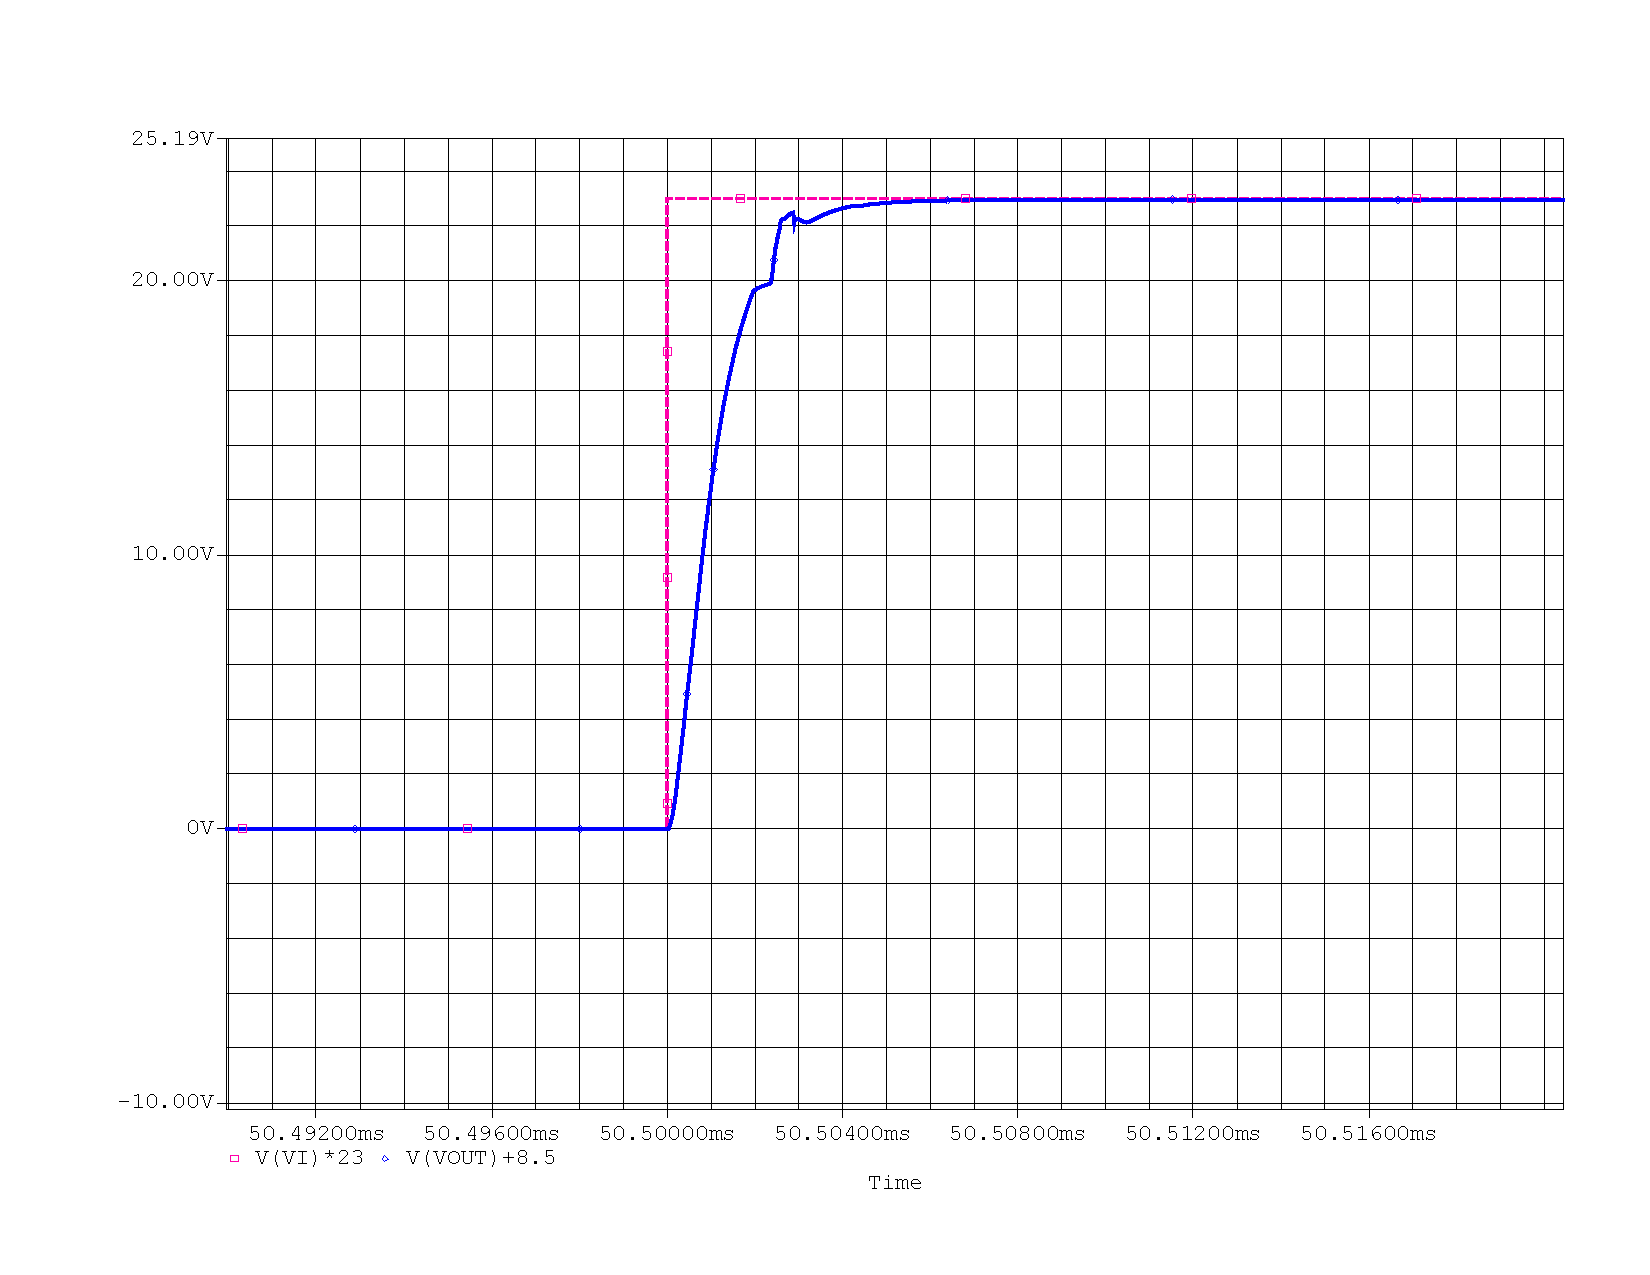
\includegraphics[scale=0.4]{sim_rta_escalon_gran_senial_zoom_sr.pdf}
%	\caption{Respuesta al escalón en gran señal ampliado.}
%	\label{fig:sim_rta_escalon_gran_sr}
%\end{figure}

	El parámetro \textit{Slew Rate} caracteriza el comportamiento de la salida del cirucito ante cambios súbitos de tensión en la entrada, ya que la tensión de salida no puede responder de forma instantánea ante alteraciones en la entrada. Para hallar su valor se impone un escalón en la entrada de gran amplitud y se mide la pendiente casi constante resultante. A partir de la figura \ref{fig:sim_rta_escalon_gran_sr} se obtiene \eqref{ec:sr}.

	\begin{equation}
	\centering
	\mathrm{SR} = \left. \frac{dV_o(t)}{dt} \right\rvert_{max} \cong \frac{\Delta V_o}{\Delta t} = \frac{\SI{27}{\volt}}{\SI{3}{\micro\second}} = \boxed{\SI{9}{\volt\per\micro\second}}
	\label{ec:sr}
\end{equation}



	
		\section{Margen de fase}\label{sec:sim_fase}
			\begin{figure}[H]
	\centering
	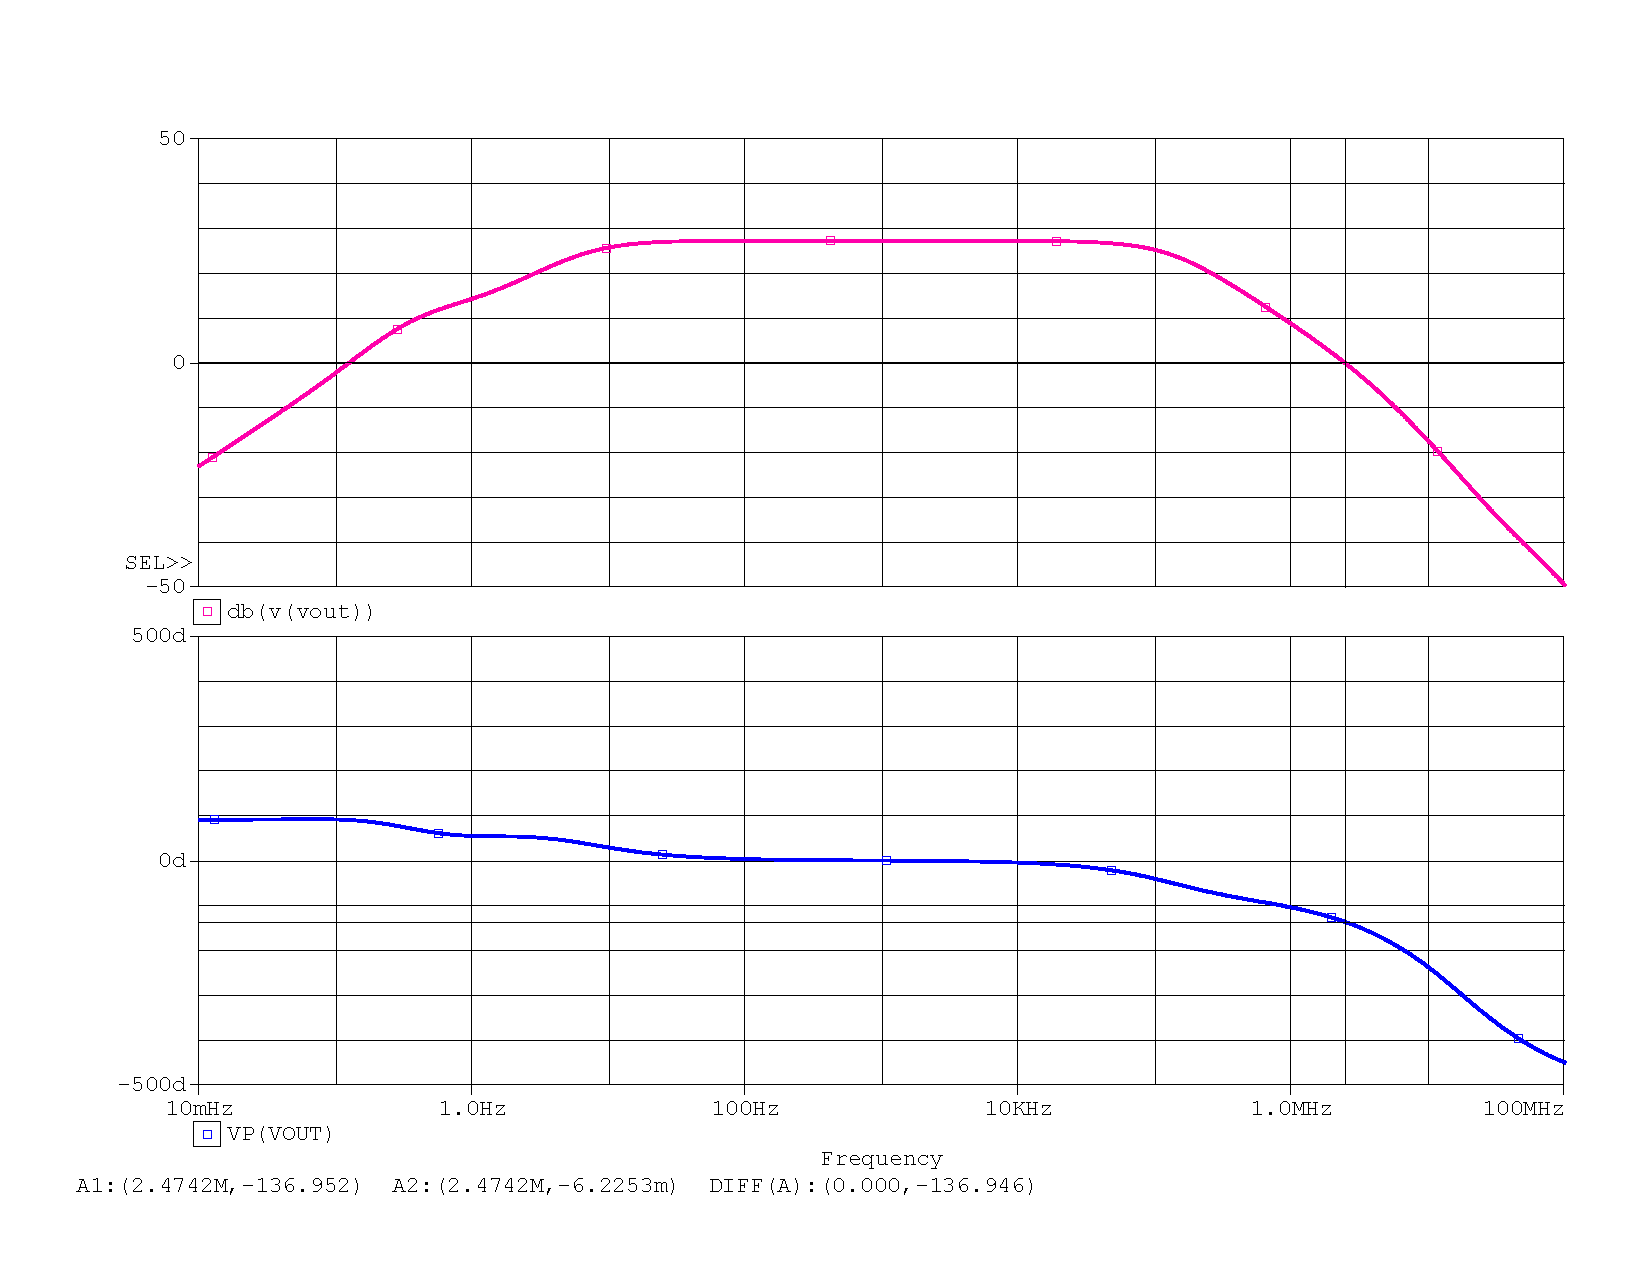
\includegraphics[scale=0.4]{sim_bode_400p.pdf}
	\caption{Diagrama de Bode.}
	\label{fig:sim_bode}
\end{figure}

En la Figura \ref{fig:sim_bode} se presentan la magnitud y fase en la salida en función de la frecuencia.
El margen de fase se define como el ángulo que le falta a \SI{-180}{\degree} para llegar a la fase cuando la ganancia es \SI{0}{\decibel}. Para determinar su valor, se busca en la Figura \ref{fig:sim_bode} el punto de cruce de la gráfica de magnitud con \SI{0}{\decibel}, que corresponde a una frecuencia de \SI{2.5}{\mega\hertz}. La fase en dicha frecuencia es de \SI{-136}{\degree}, por lo que el margen de fase resulta:

	$$ \mathrm{MF} = \SI{-180}{\degree} + \SI{136}{\degree} = \boxed{\SI{-44}{\degree}} $$

		\section{Distorsión armónica}\label{sec:sim_thd}
				Mediante la herramienta de análisis de Fourier provista por \texttt{SPICE Orcad} se analizó la variación de la distorsión armónica \texttt{THD} producida en la salida, en función de la frecuencia y amplitud de la señal de entrada. Los resultados obtenidos se resumen en la tabla.

\begin{table}[H]
	\centering
	\begin{tabular}{ccccc}
		\toprule
\multirow{2}{*}{Frecuencia} & \multicolumn{3}{c}{$P_{L,RMS}$} \\ 
		\cmidrule{2-4}
			& 4W & 30W & 42,5W \\
		\midrule
		\SI{1}{\kHz} & \num{0,005} & \num{0,016} & \num{0,018} \\
		\SI{20}{\kHz} & \num{0.053} & \num{0,066} & \num{0,099} \\
		\bottomrule
	\end{tabular}
	\caption{Valores de $\mathrm{THD}_{\%}$ para distintos valores de frecuencia y potencias sobre la carga.}
\end{table}


\begin{figure}[H]
	\centering
	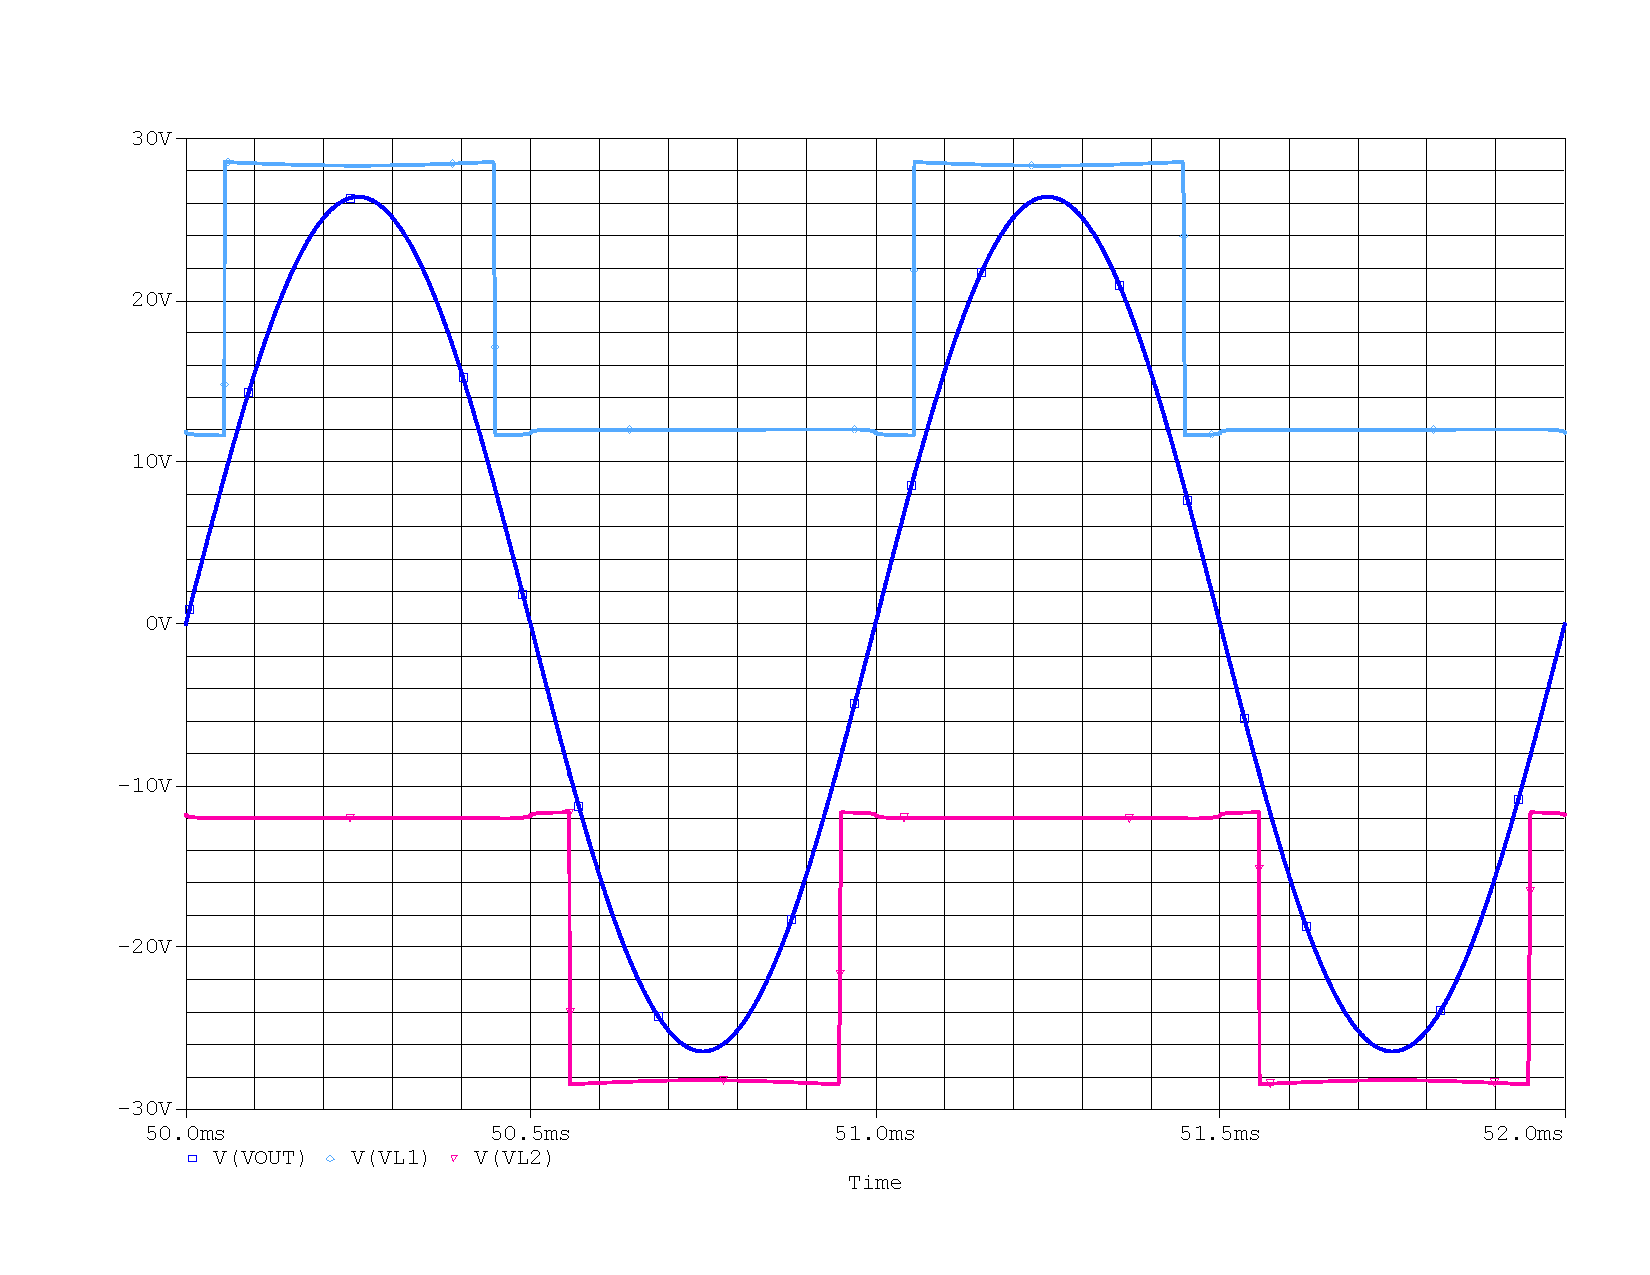
\includegraphics[scale=0.4]{sim_salida1k_max.pdf}
	\caption{Máxima excursión de salida sin recorte a \SI{1}{\kilo\hertz} $THD = \num{0.018}\%$.}
	\label{fig:sim_salida_1k_max}
	\end{figure}

\begin{figure}[H]
	\centering
	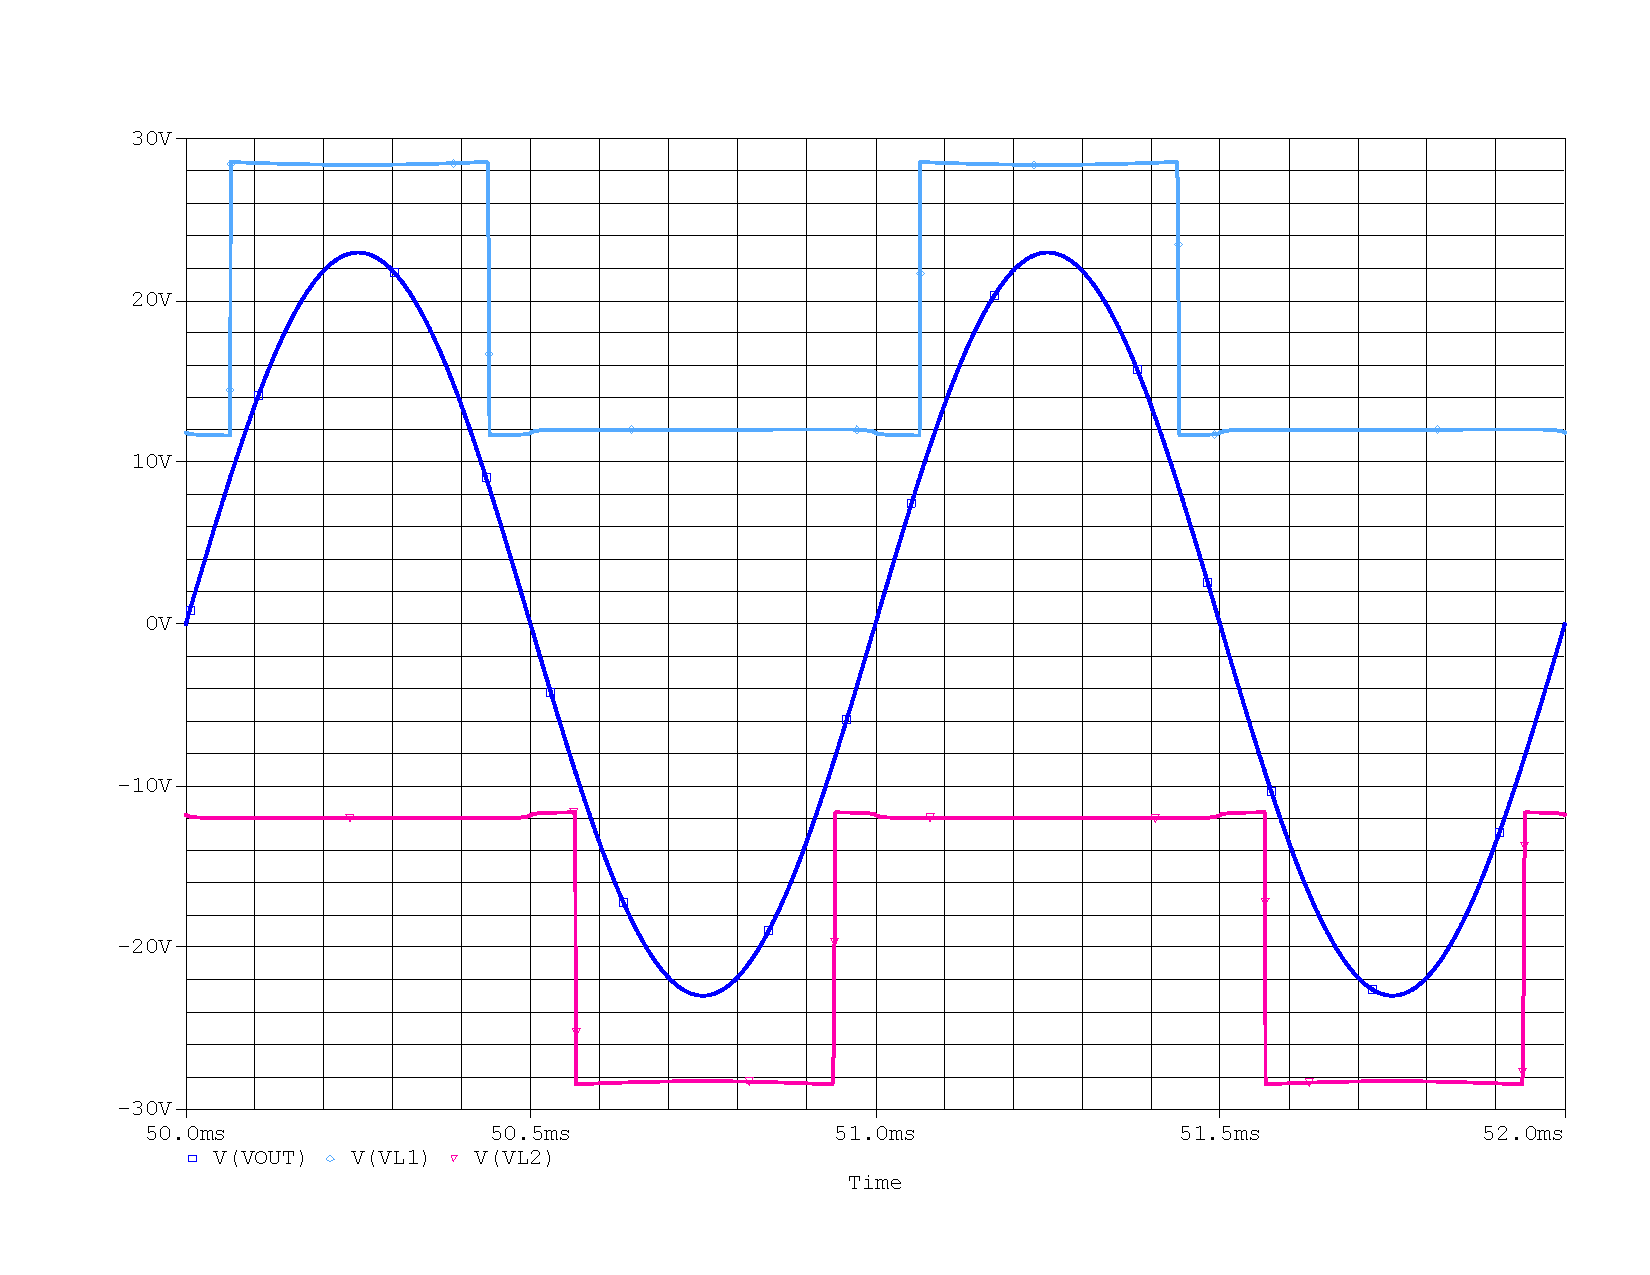
\includegraphics[scale=0.4]{sim_salida_1k_22V.pdf}
	\caption{22V, 1V, $THD=\num{0.016}\%$.}
	\end{figure}

\begin{figure}[H]
	\centering
	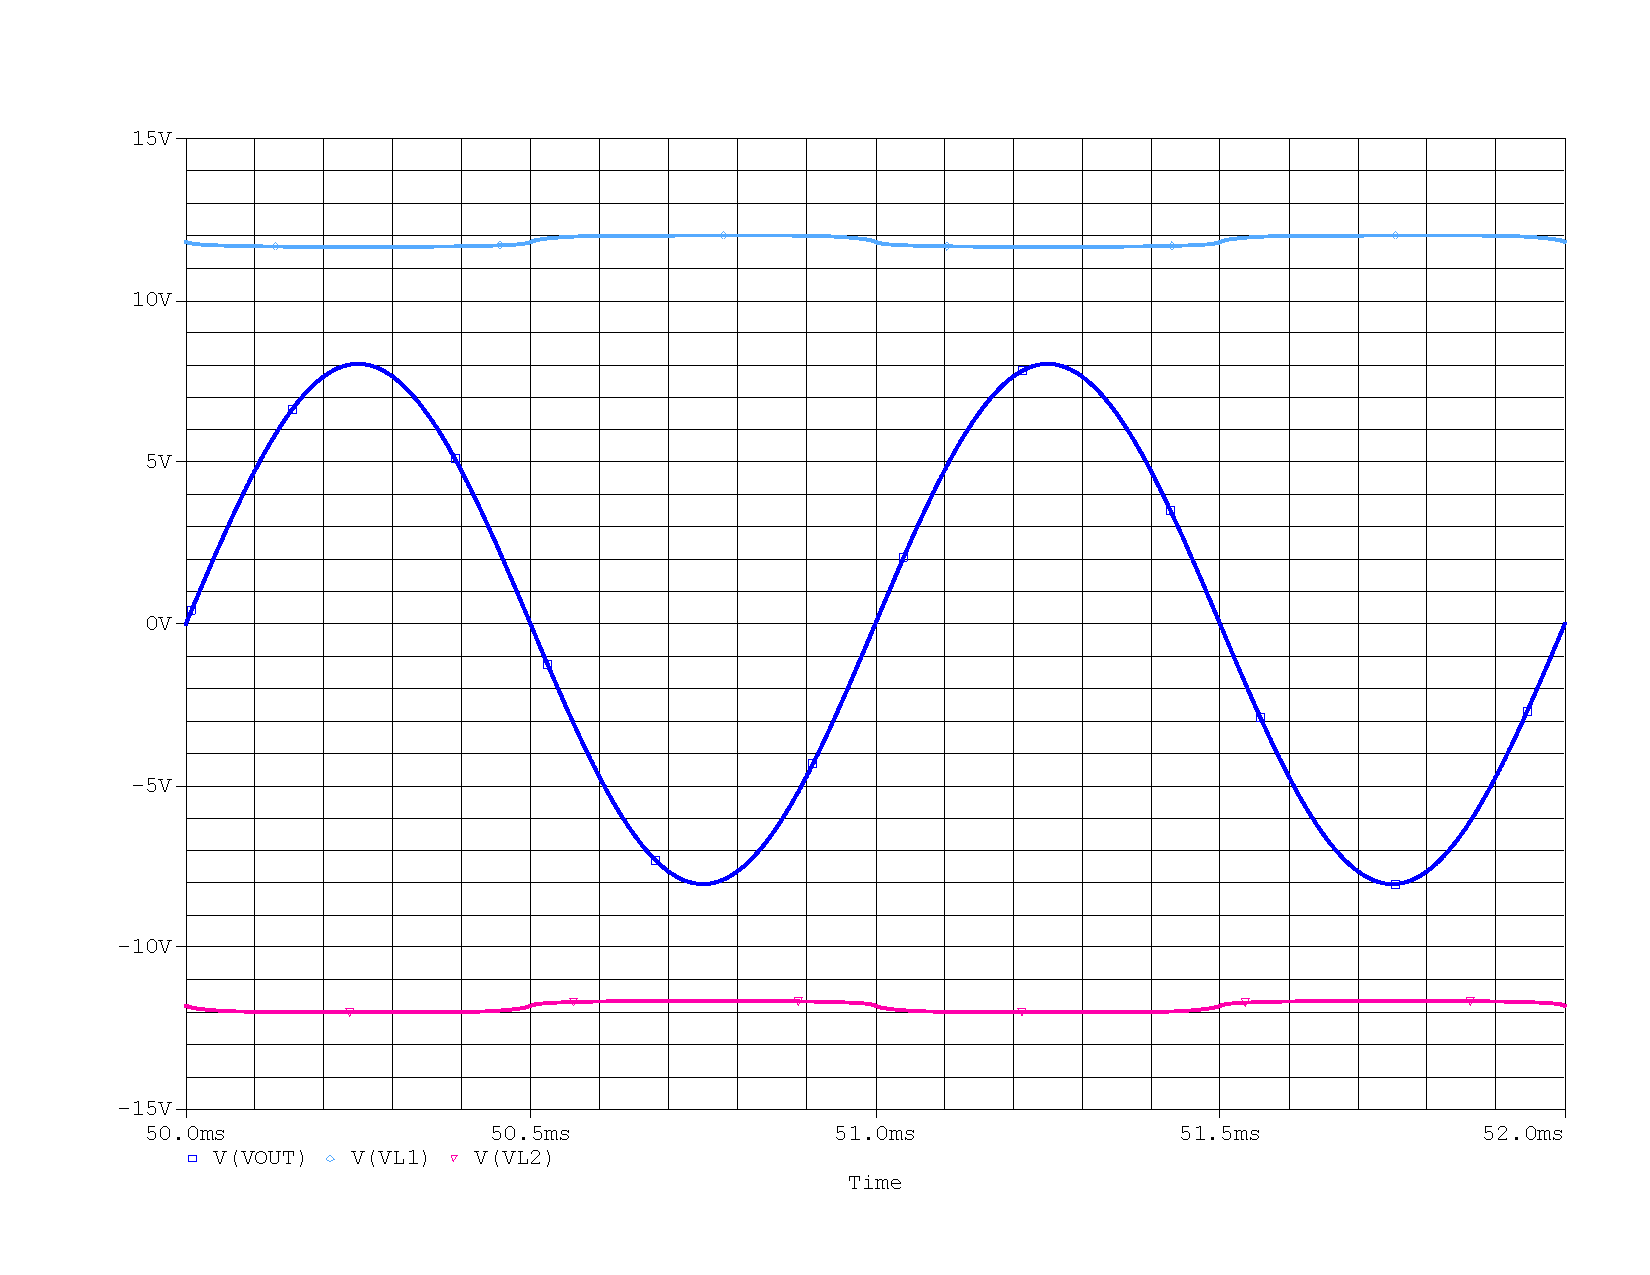
\includegraphics[scale=0.4]{sim_salida_1k_8V.pdf}
	\caption{8V, $\SI{.35}{\V}$, $THD=\num{0.005}\%$.}
\end{figure}

%%%% 20kHz
\begin{figure}[H]
	\centering
	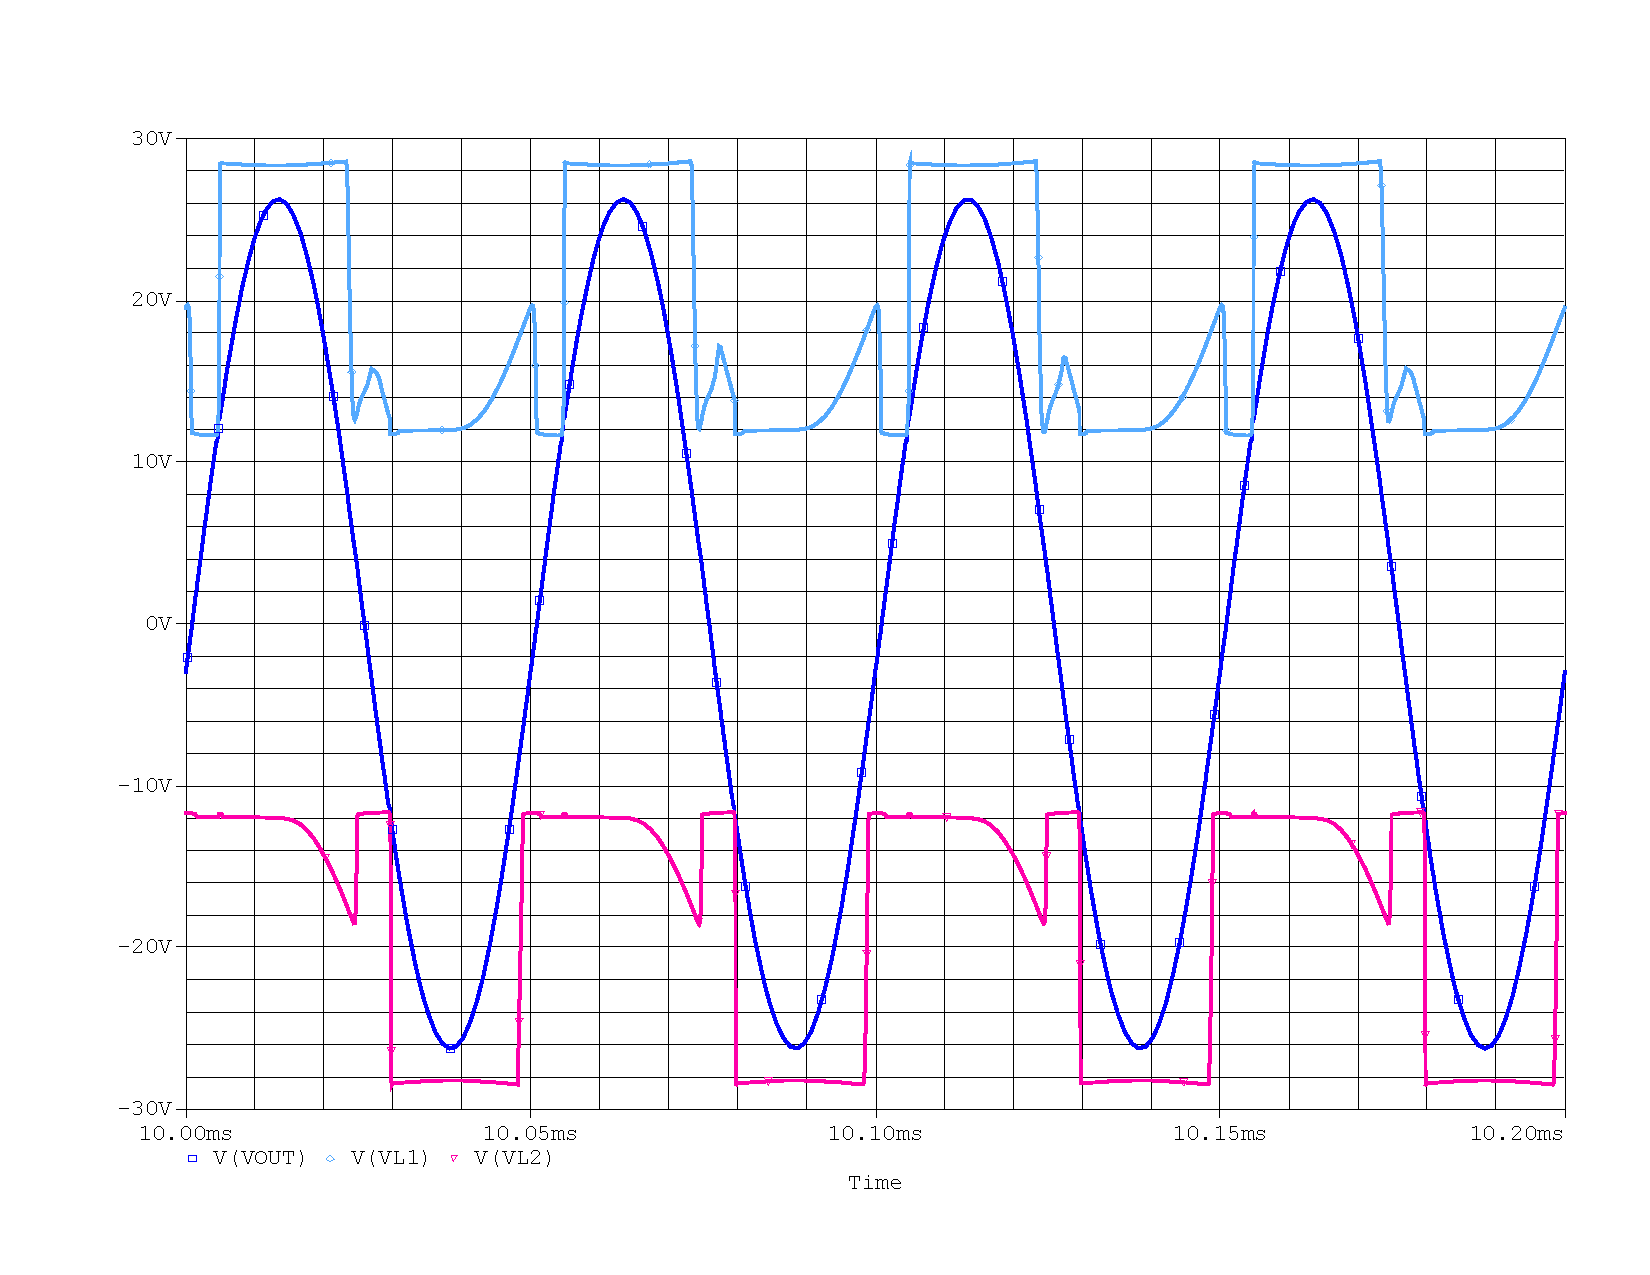
\includegraphics[scale=0.4]{sim_salida_20k_max.pdf}
	\caption{\SI{26.1}{\V}, \SI{0.35}{\V}, $THD=\num{0.053}\%$.}
\end{figure}

\begin{figure}[H]
	\centering
	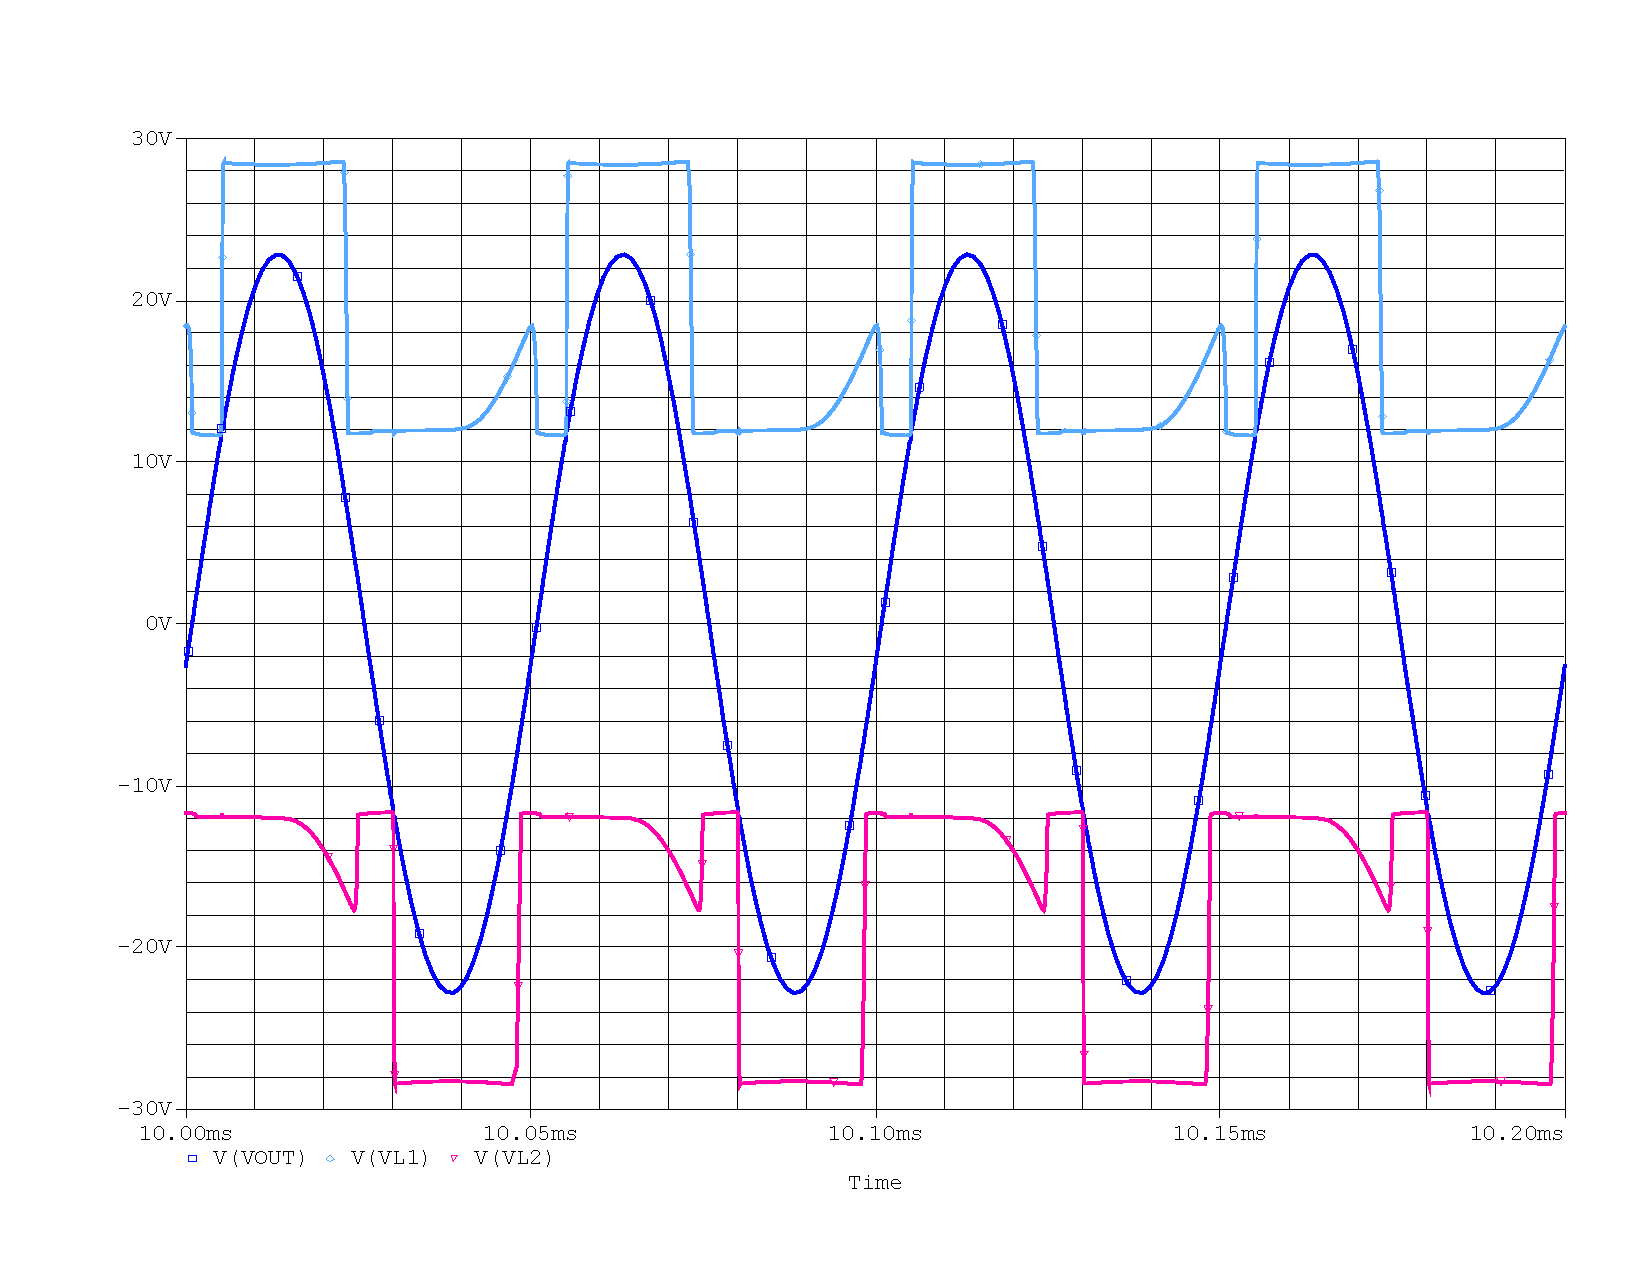
\includegraphics[scale=0.4]{sim_salida_20k_22V.pdf}
	\caption{\SI{22}{\V}, \SI{1}{\V}, $THD=\num{0.066}\%$.}
\end{figure}

\begin{figure}[H]
	\centering
	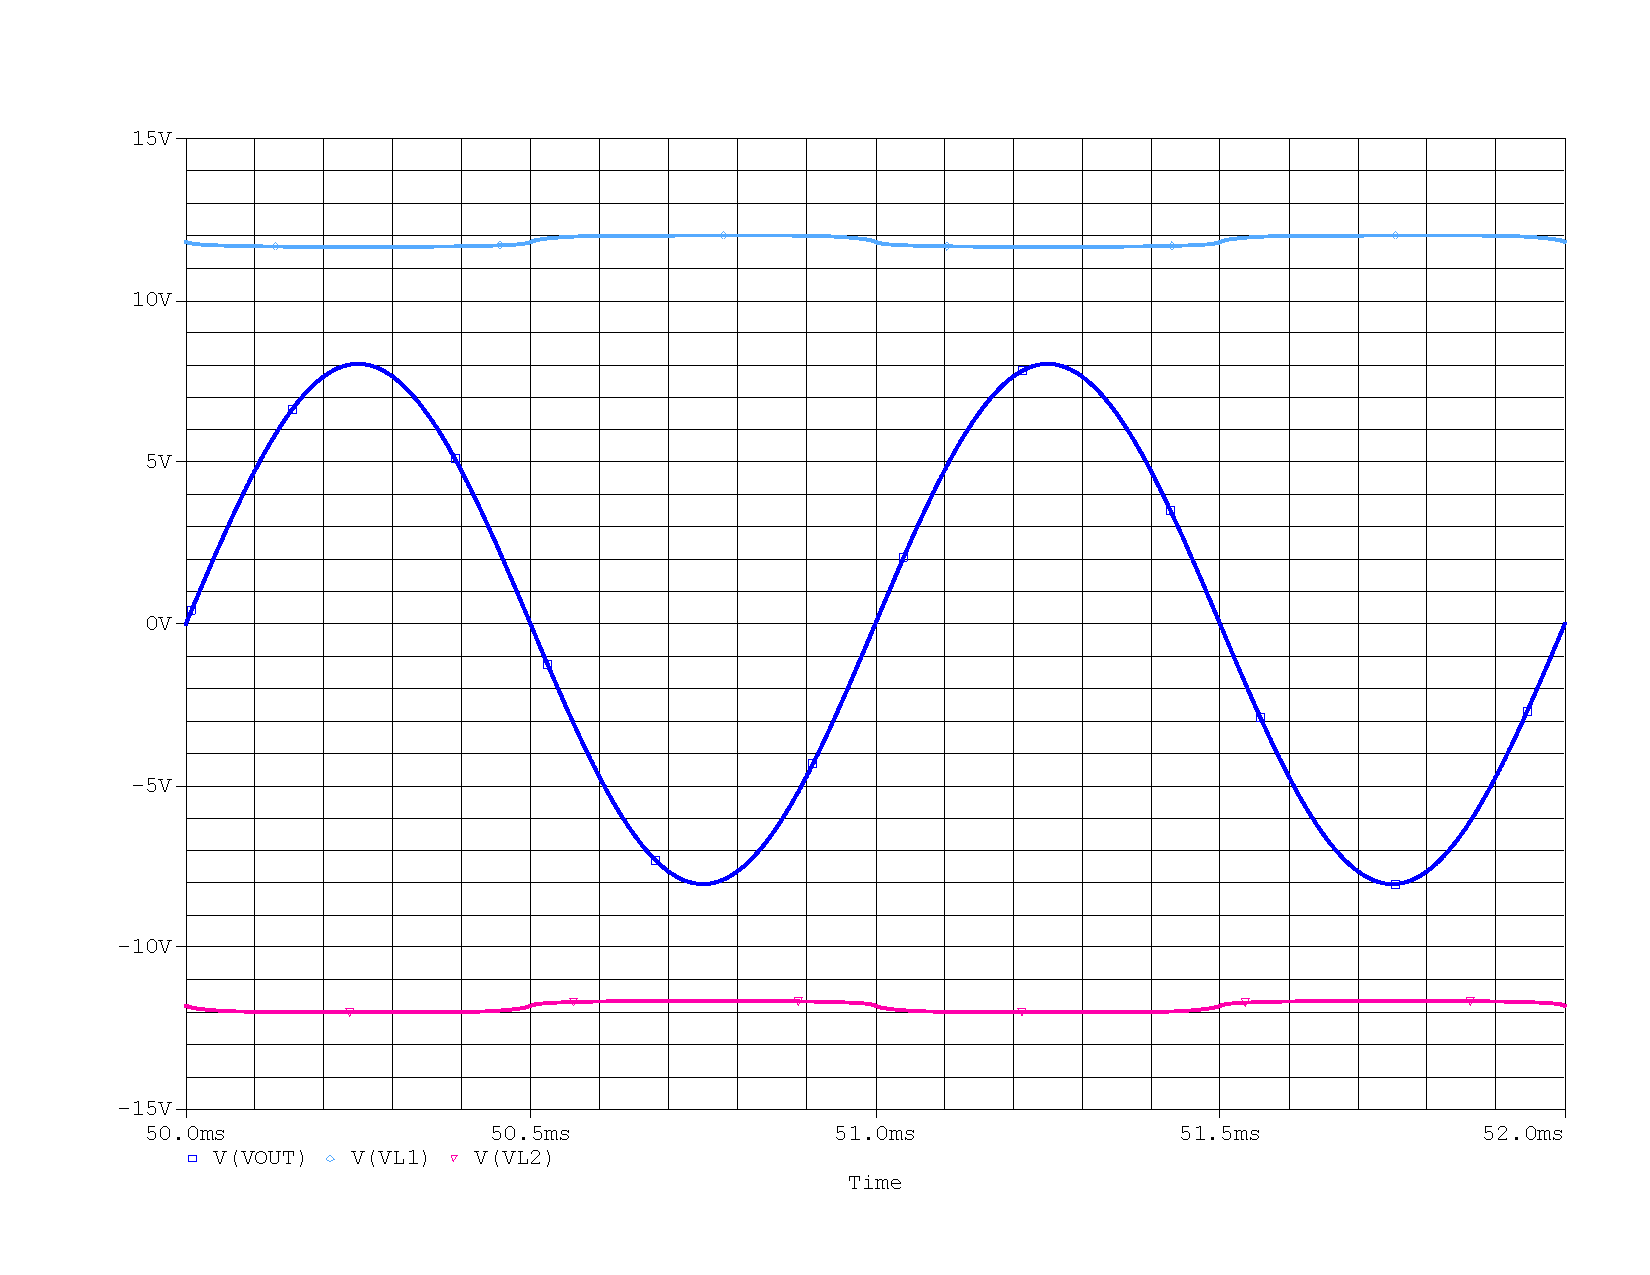
\includegraphics[scale=0.4]{sim_salida_1k_8V.pdf}
	\caption{\SI{8}{\V}, \SI{0.35}{\V}, $THD=\num{0.099}\%$.}
\end{figure}





		
		\section{Distorsión por intermodulación}\label{sec:sim_intermod}
			
Para esta simulación se utilizaron dos señales de entrada superpuestas, una de frecuencia de \SI{100}{\Hz} con amplitud pico \SI{0.4}{\volt} y una de \SI{5}{\kHz} con \SI{0.1}{\volt}, y se mide la distorsión en \SI{5}{\kHz} con los mismos procedimientos de la medición anterior, obteniéndose 
$$ \mathrm{IMD} = 1,4\% $$

%Los resultados obtenidos se muestran en la tabla \ref{tab.intermod}

%\begin{table}[H]
%	\centering
%	\begin{tabular}{ccccc}
%		\toprule
%\multirow{2}{*}{Frecuencia} & \multicolumn{3}{c}{$P_L$} \\ 
%		\cmidrule{2-4}
%			& 4W & 30W & 42W \\
%		\midrule
%		 \SI{11}{\kHz} & \num{2.14} & \num{2.15} & \num{2.15}\\
%		 \bottomrule
%	\end{tabular}
%	\caption{Valores porcentuales de distorsión de intermodulación para distintos valores de frecuencia y potencias sobre la carga.}
%	\label{tab.intermod}
%\end{table}


		\section{Rechazo de Ruido de la Fuente de Alimentación}\label{sec:sim_psnr}
			La relación de rechazo de la fuente de alimentación da una medida del rechazo del ruido proveniente de la fuente de alimentación que puede proveer el circuito para distintas frecuencias. En la simulación, se anexó una fuente alterna en serie con cada fuente de alimentación y se pasivó la señal de entrada. Se realizó un barrido en frecuencia con una amplitud \SI{1}{\volt}, obteniendose diversas amplitudes en la salida, según se ilustra en la Figura \ref{fig:psrr}.
\begin{figure}[H]
	\centering
	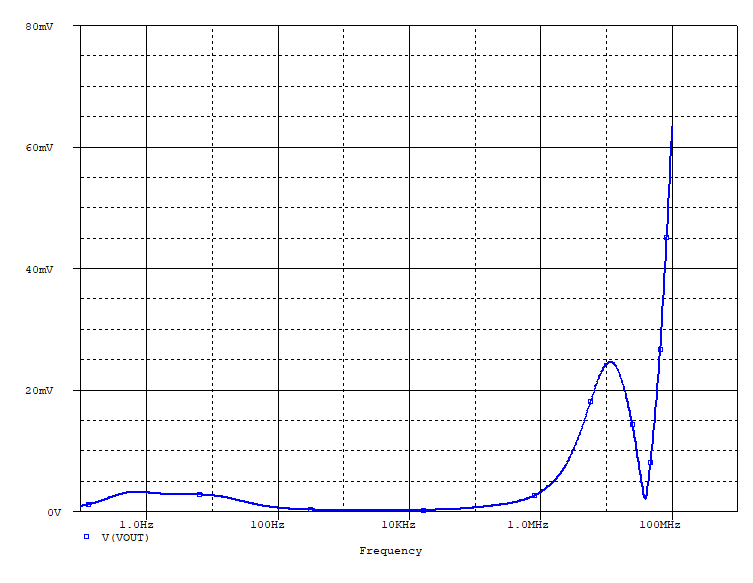
\includegraphics[scale=0.3]{sim_psrr}
	\caption{Rechazo de Ruido de la Fuente.}
	\label{fig:psrr}
\end{figure}

$$ \mathrm{PSRR} [\%]= \frac{v_o}{v_i} = \frac{\SI{2}{\milli\volt}}{\SI{1}{\volt}} = \num{0,002} \%$$
$$ \mathrm{PSRR} [\SI{}{\decibel}] = 20 \cdot \log \left( \frac{\SI{2}{\milli\volt}}{\SI{1}{\volt}} \right) = \SI{-54}{\decibel} $$

		\section{Máxima eficiencia del amplificador}\label{sec:max_ef}
			
La eficiencia de un circuito se define como la relación entre la potencia promedio entregada a la carga (PL) y la potencia consumida por la fuente de alimentación ($P_{fuente}$). El cálculo es análogo al de clase B, salvo que en un clase G, la disipación de potencia es compartida entre dos transistores, y la disipación en los transistores externos es cero cuando no se supera la tensión umbral.

\begin{equation}
	\centering
	\nu = \frac{P_L}{P_{fuente}} = \frac{\pi}{4} \cdot \frac{\hat{V}_o}{V_{CC}} = \frac{\pi}{4} \cdot \frac{26}{30}= \boxed{68\%}
\end{equation}

Siendo $ \hat{V}_o$ máxima tensión de salida sin que haya recorte.

\HgraficarPNG{0.5}{potencia}{Potencia disipada en la carga y transistores de salida.}{fig.potencia}

En la Figura \ref{fig.potencia} se muestra la potencia disipada en la carga, siendo la máxima (sin distorsión) \SI{86}{\watt}, la curva rosa corresponde al transistor externo $Q_{62}$, $P_{max} = \SI{18}{\watt}$. La curva azul, la potencia disipada en el transistor interno de salida $Q_{63}$.




		\section{Cálculo de Disipadores}\label{sec:sim_disipadores}
				A partir de la hoja de datos del \texttt{TIP41} y de las condiciones del ambiente se tiene:
	\begin{itemize}
		\item  Temperatura de Juntura $T_j = \SI{150}{\celsius} $
		\item  Temperatura de Carcasa $T_c = \SI{25}{\celsius} $
		\item  Temperatura de Ambiente $T_a = \SI{40}{\celsius} $
		\item  $\theta_{cs} = \SI{1}{\celsius\per\W}$ 
		%	\Gus{Esto es porque uno usa mica $\SI{2}{\celsius\per\W}$ y el otro no $\SI{0.5}{\celsius\per\W} - \SI{1}{\celsius\per\W}$}
		\item  Disipación total del \texttt{TIP41} a $T_{case} = \SI{25}{\celsius}$ se obtiene $\theta_{jc} =  \frac{T_j - T_c}{P_{Ctip41_{\max}}} =\SI{1.92}{\celsius\per\W}$ 
		\\	se usa el mas grande para no forzar tanto al TIP ( de esta forma te queda un disipador mas grande)
	\end{itemize}

	Dado estos valores se puede hallar:

	\begin{equation}
		P_{C_{\max}} = \frac{V^2_{CC}}{\pi^2 R_L} = \SI{11.4}{\W}
	\end{equation}

	\begin{equation}
		\theta_{ja} =  \frac{T_j - T_a}{P_{C_{\max}}} =\SI{9.65}{\celsius\per\W}
	\end{equation}
	

	\begin{equation}
		\theta_{ja} = \theta_{jc} + \theta_{cs} + \theta_{sa}
	\end{equation}

	Despejando:

	\begin{equation}
		\theta_{sa} = \theta_{ja} - \theta_{jc} - \theta_{cs} = \boxed{\SI{6.72}{\celsius\per\W}}
	\end{equation}

	Buscando disipadores en \url{www.disipadores.com} se halló que el \texttt{Z36} es el más cercano a las especificaciones requeridas (con $\theta$ alrededor de \SI{8.5}{\celsius\per\W}). Otra alternativa es el disipador con aletas \texttt{Z66} que es más largo y tiene $\theta = \SI{7.5}{\celsius\per\W}$.



%	\pagebreak
		\section{Resultados}
			\begin{table}[H]
	\centering
	\begin{tabular}{ccc}
		\toprule
		& Especificaciones & Simulaciones \\
		\midrule
		 THD a Prms \SI{39}{\watt} \SI{1}{\kilo\hertz}& $< 0,02\%$ &  0,018\% \\
		 THD a \SI{1}{\watt}, \SI{1}{\kilo\hertz} & $< 0,01\%$ & 0,005\% \\
		 Respuesta en frecuencia & \SI{20}{\hertz} a \SI{20}{\kilo\hertz} & \SI{14}{\hertz} a \SI{156}{\kilo\hertz} \\
		 Tensión de \textit{offset} & \SI{5}{\milli\volt} & \SI{2.5}{\milli\volt} \\
		 \textit{Slew Rate} & \SI{10}{\volt\per\micro\second} &  \SI{9}{\volt\per\micro\second} \\
		 IMD & 1\% & 1,4\% \\
		 Margen de Fase & \SI{45}{\degree} &  \SI{44}{\degree} \\
		 Factor de amortiguamiento & $>500$ & 3333 \\
		 Impedancia de entrada & \SI{100}{\kilo\hertz} & \SI{94}{\kilo\hertz} \\
		 Impedancia de salida & \SI{}{\milli\ohm} & \SI{2.4}{\milli\ohm}\\
		\bottomrule
	\end{tabular}
	\caption{Resultados.}
	\label{tab.resultados}
\end{table}

%	\pagebreak

%	\part{Construcción del prototipo}\label{part:construccion}
%		\Juan{Ver pdf ''Grupo01\_informe\_final`` como referencia}
%		
	\subsection{Selección de los transistores}
		Durante el proceso de soldado de componentes, se compraron varios transistores iguales con el fin de obtener su $\beta$. Aquellos transistores que tengan $\beta$ similares, se les procedió a ver la relación $V_{BE}$ vs $I_{CQ}$. Para ello, se conectaron los transistores en modo diodo y se les conectó una fuente y una resistencia serie para limitar la corriente. Por los mismos circulará la misma corriente y ahí se mide el $V_{BE}$ de cada uno.

	Fuente 68.

	Cuando hagamos la etapa de salida, hay que estañar las pistas de salida porque quedaron un poco finas y en vez de agrandar de grosor las agrandamos de altura.


	\subsection{Validación del prototipo}

		Mediciones de polarización:

		Vbe del multiplicador de Vbe $= \SI{.55}{\volt}$
		Vce del multiplicador de Vbe $= \SI{2.1}{\volt}$
		110 y 208 millivolt en las re de la carga activa
		Caida en R12 (resistencia del emisor (2.2k) del PD) $= \SI{8}{\volt}$
		
		\Juan{Comprar: cables para los transistores, fichas jack de celular y de guitarra para la placa, disipador, patitas mayores a 2cm de separadores (los plasticos que sostienen a la placa)}


	\part{Validación del prototipo}\label{part:mediciones}
		\section{Instrumentos utilizados}
			
	Las mediciones se realizaron con el siguiente instrumental provisto por los laboratorios de la Facultad de Ingeniería de la UBA.

	\graficarPNG{0.8}{instru_M10SP3010E}{Fuente de alimentación \emph{M10SP3010E}.}{fig:M10SP3010E}
	\graficarPNG{0.8}{instru_ADS1102CAL}{Osciloscopio \emph{ATTEN ADS1102CAL}.}{fig:ADS1102CAL}
%	\graficarPNG{0.6}{instru_RIGOL_DS1102E}{Osciloscopio \emph{RIGOL DS1102E}.}{fig:RIGOL_DS1102E}
	\graficarPNG{0.3}{instru_UT30D}{Multímetro \emph{UT30D}.}{fig:UT30D}
	\graficarPNG{0.3}{instru_FG_8002}{Generador de funciones \emph{FG 8002}.}{fig:FG_8002}
	
	% Para medir inductancias usamos PROTOMAX VA511
	\graficarPNG{0.1}{instru_PROTOMAX_VA511}{Medidor de LCR portátil \emph{PROTOMAX VA511}.}{fig:VA511}


		\section{Validación y resultados}
			
	\subsection{Circuito sin etapa de potencia}
		A continuación se exponen las mediciones realizadas los días \texttt{4/12/2018} y \texttt{5/12/2018} donde se valida el funcionamiento de la primer y segunda etapa del circuito. Para realizar las mismas, se desconectan las conexiones del multiplicador de $V_{BE}$ con los transistores de salida; también se conecta la realimentación global a la salida del VAS dado que el mismo provee la misma tensión que la salida del circuito completo. Sin embargo para emular la conexión de la tercer etapa, se conecta una resistencia de valor comercial \SI{39}{\kilo\ohm} que es aproximadamente igual a la carga que presenta la reflexión de $R_L$ (con valor teórico de \SI{36}{\kilo\ohm}).\\
		\indent Con dichas consideraciones se procede a realizar las mediciones.
		\graficarEPS{0.6}{banco_med}{Diagrama del circuito para mediciones sin etapa de potencia.}{fig:banco_med}

		\subsubsection{Polarización}
		
		Las mediciones de polarización se realizaron con el multímetro \emph{UT30D} cortocircuitando la entrada y se exponen en la Figura \ref{fig:51218_pol}. Cabe destacar que las mediciones en color rojo corresponden a tensiones con respecto a masa y aquellas en color azul, diferencia de potencial.
		
		\begin{figure}[h!]
			\centering
			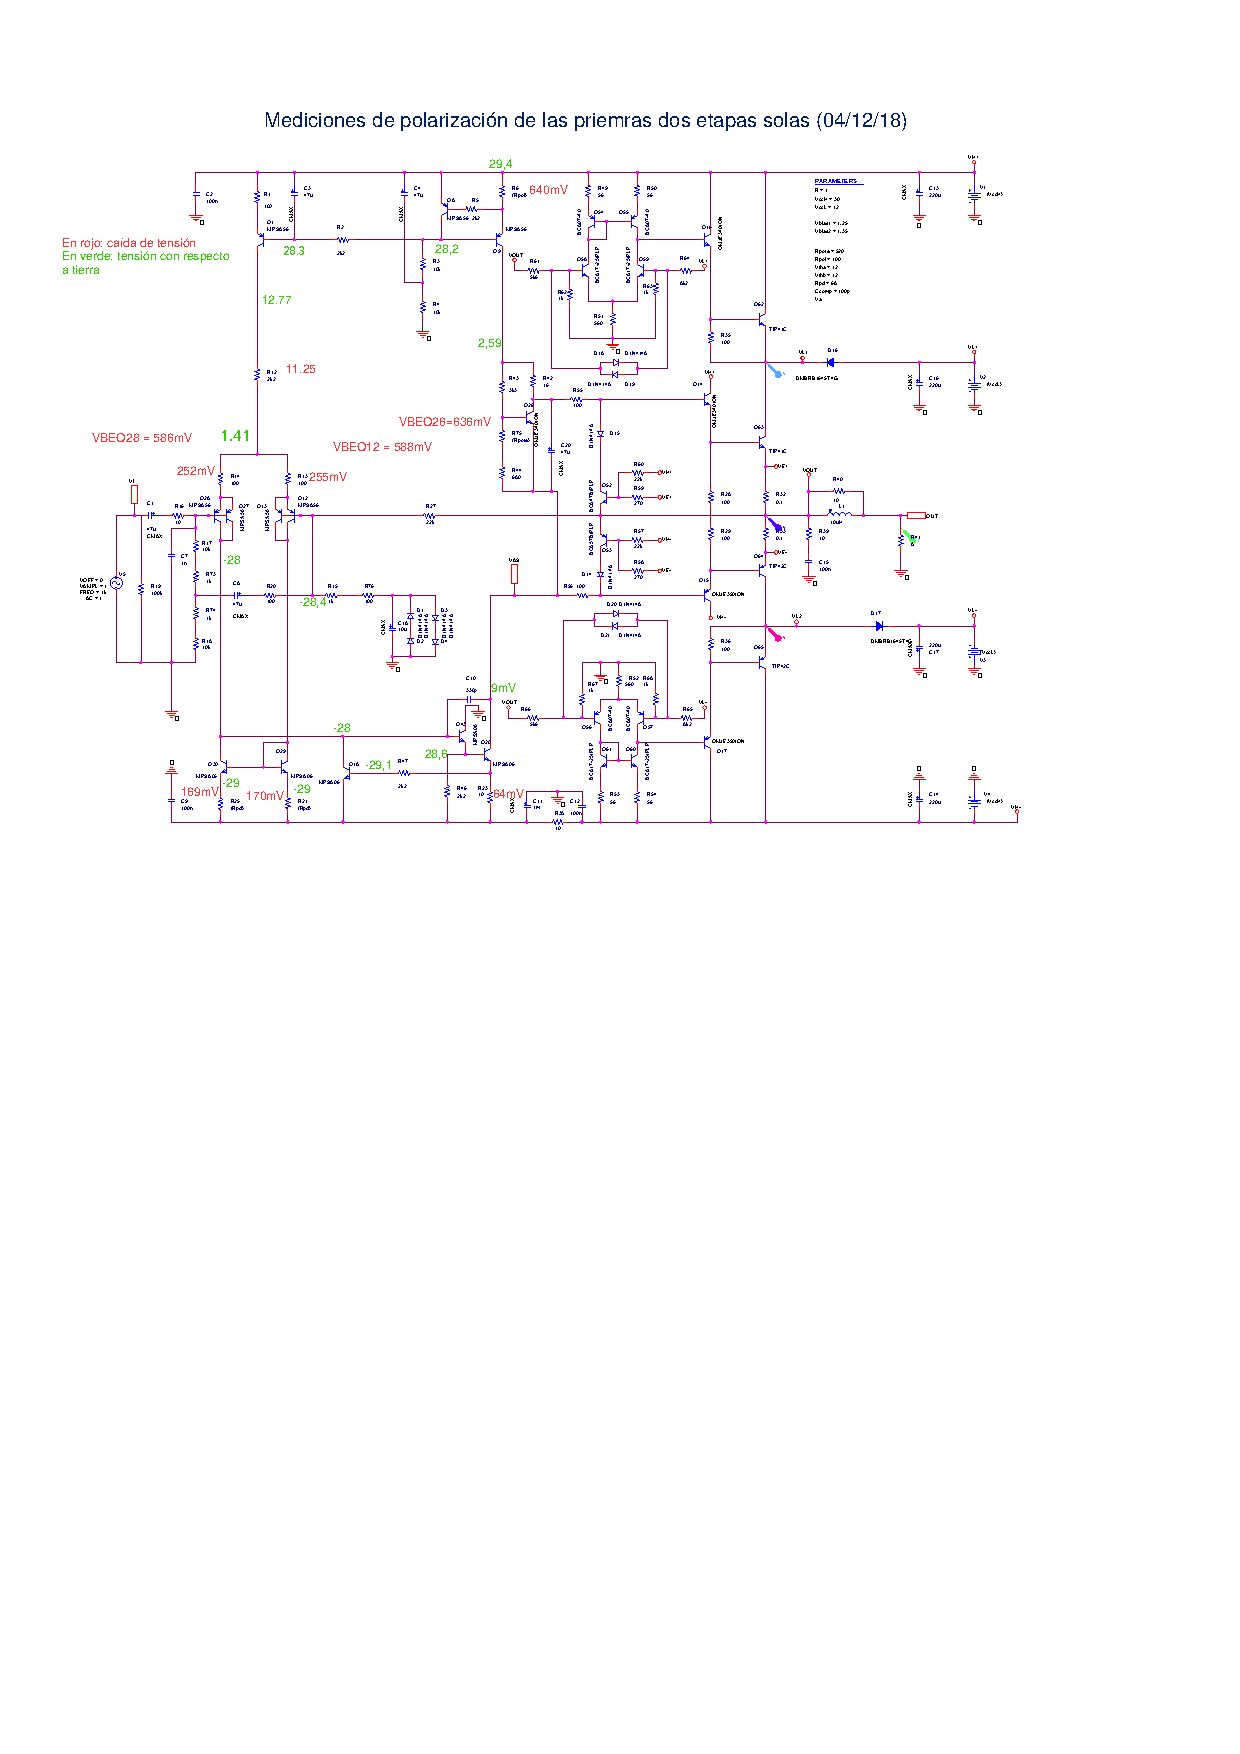
\includegraphics[angle=-90, scale=0.6]{./Mediciones/1_mediciones.pdf}
			\caption{Mediciones de polarización del día \texttt{4/12/2018}.}
			\label{fig:51218_pol}
		\end{figure}
		
		%\begin{figure}[h!]
		%	\centering
		%	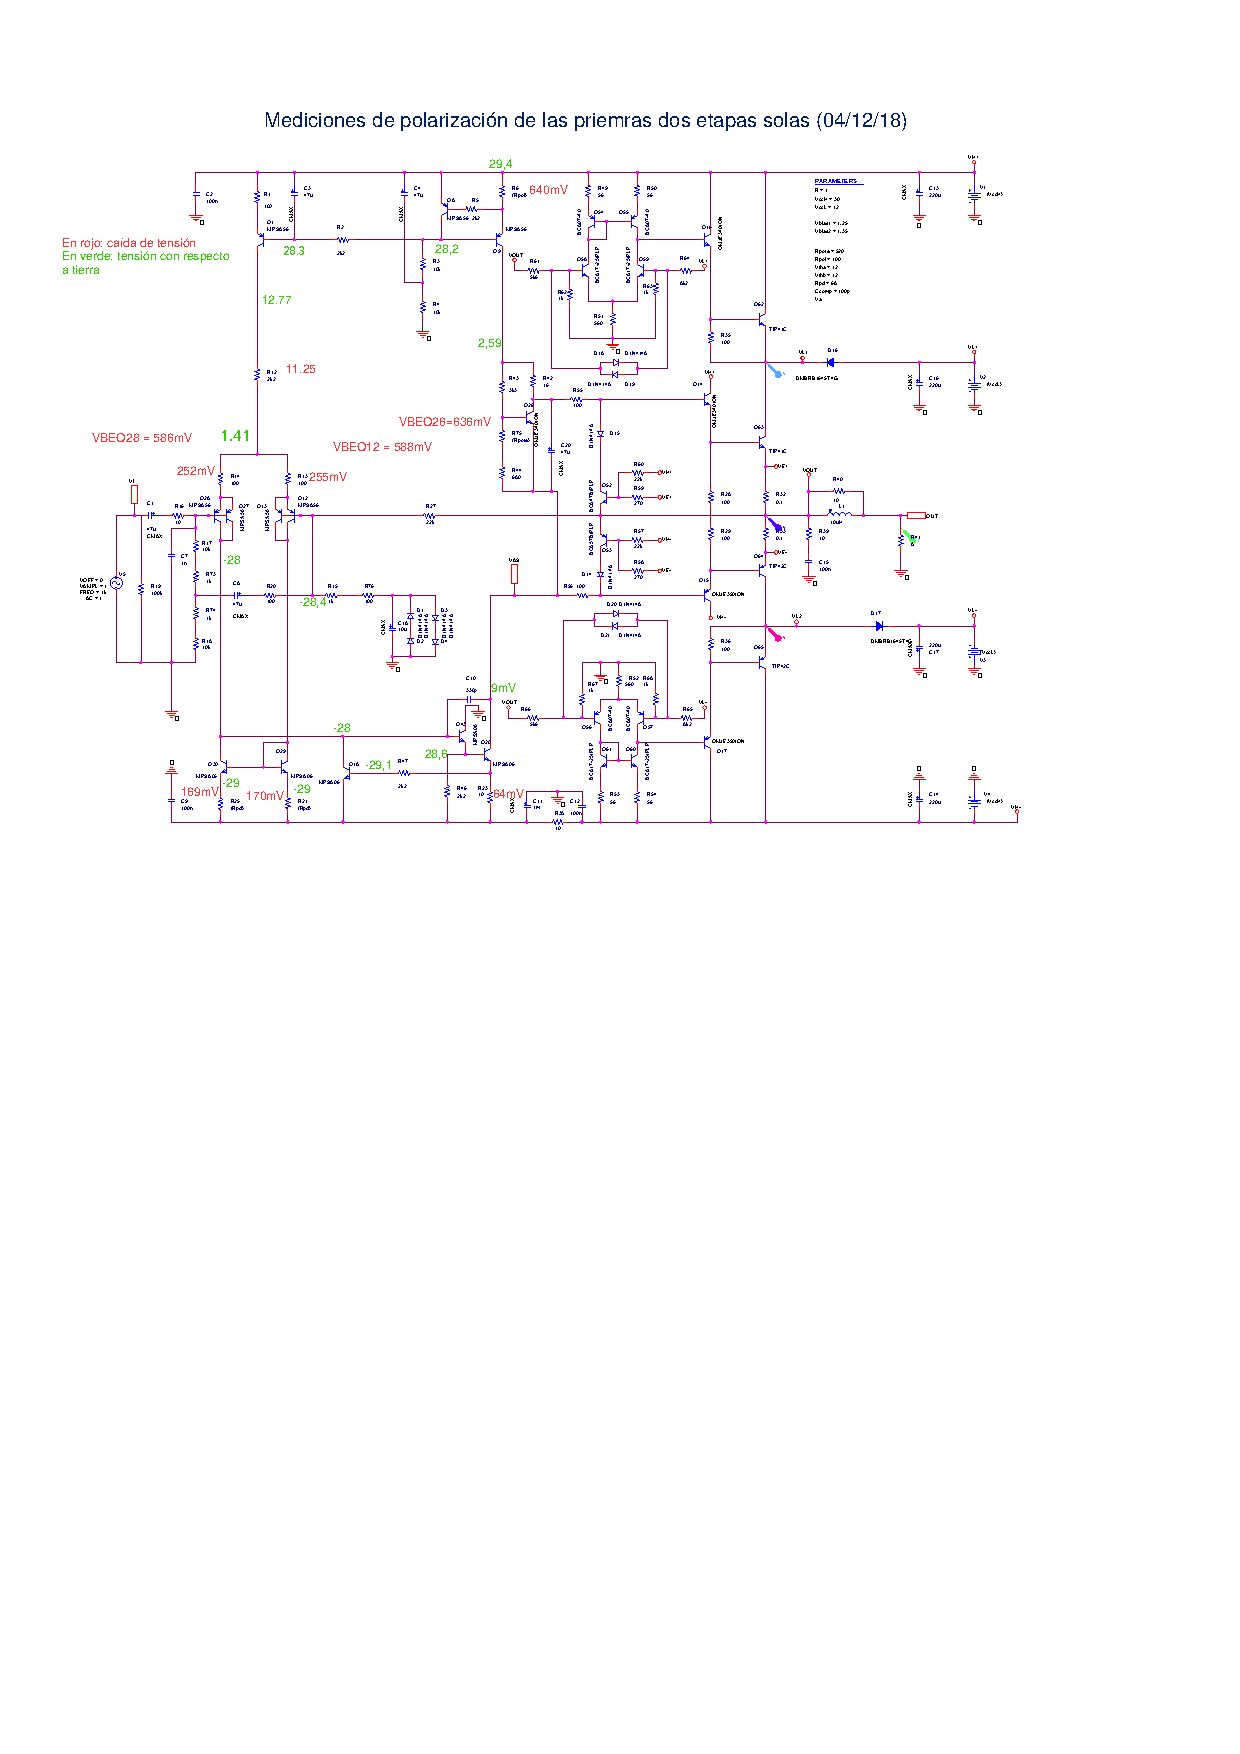
\includegraphics[width=0.8\textwidth, trim = 2cm 14cm 4cm 1cm]{./Mediciones/1_mediciones.pdf}
		%	\caption{Mediciones de polarización del día \texttt{4/12/2018}.}
		%	\label{fig:51218_pol}
		%\end{figure}

		\subsubsection{Impedancia de entrada}
			
		\begin{figure}[ H]
			\centering
			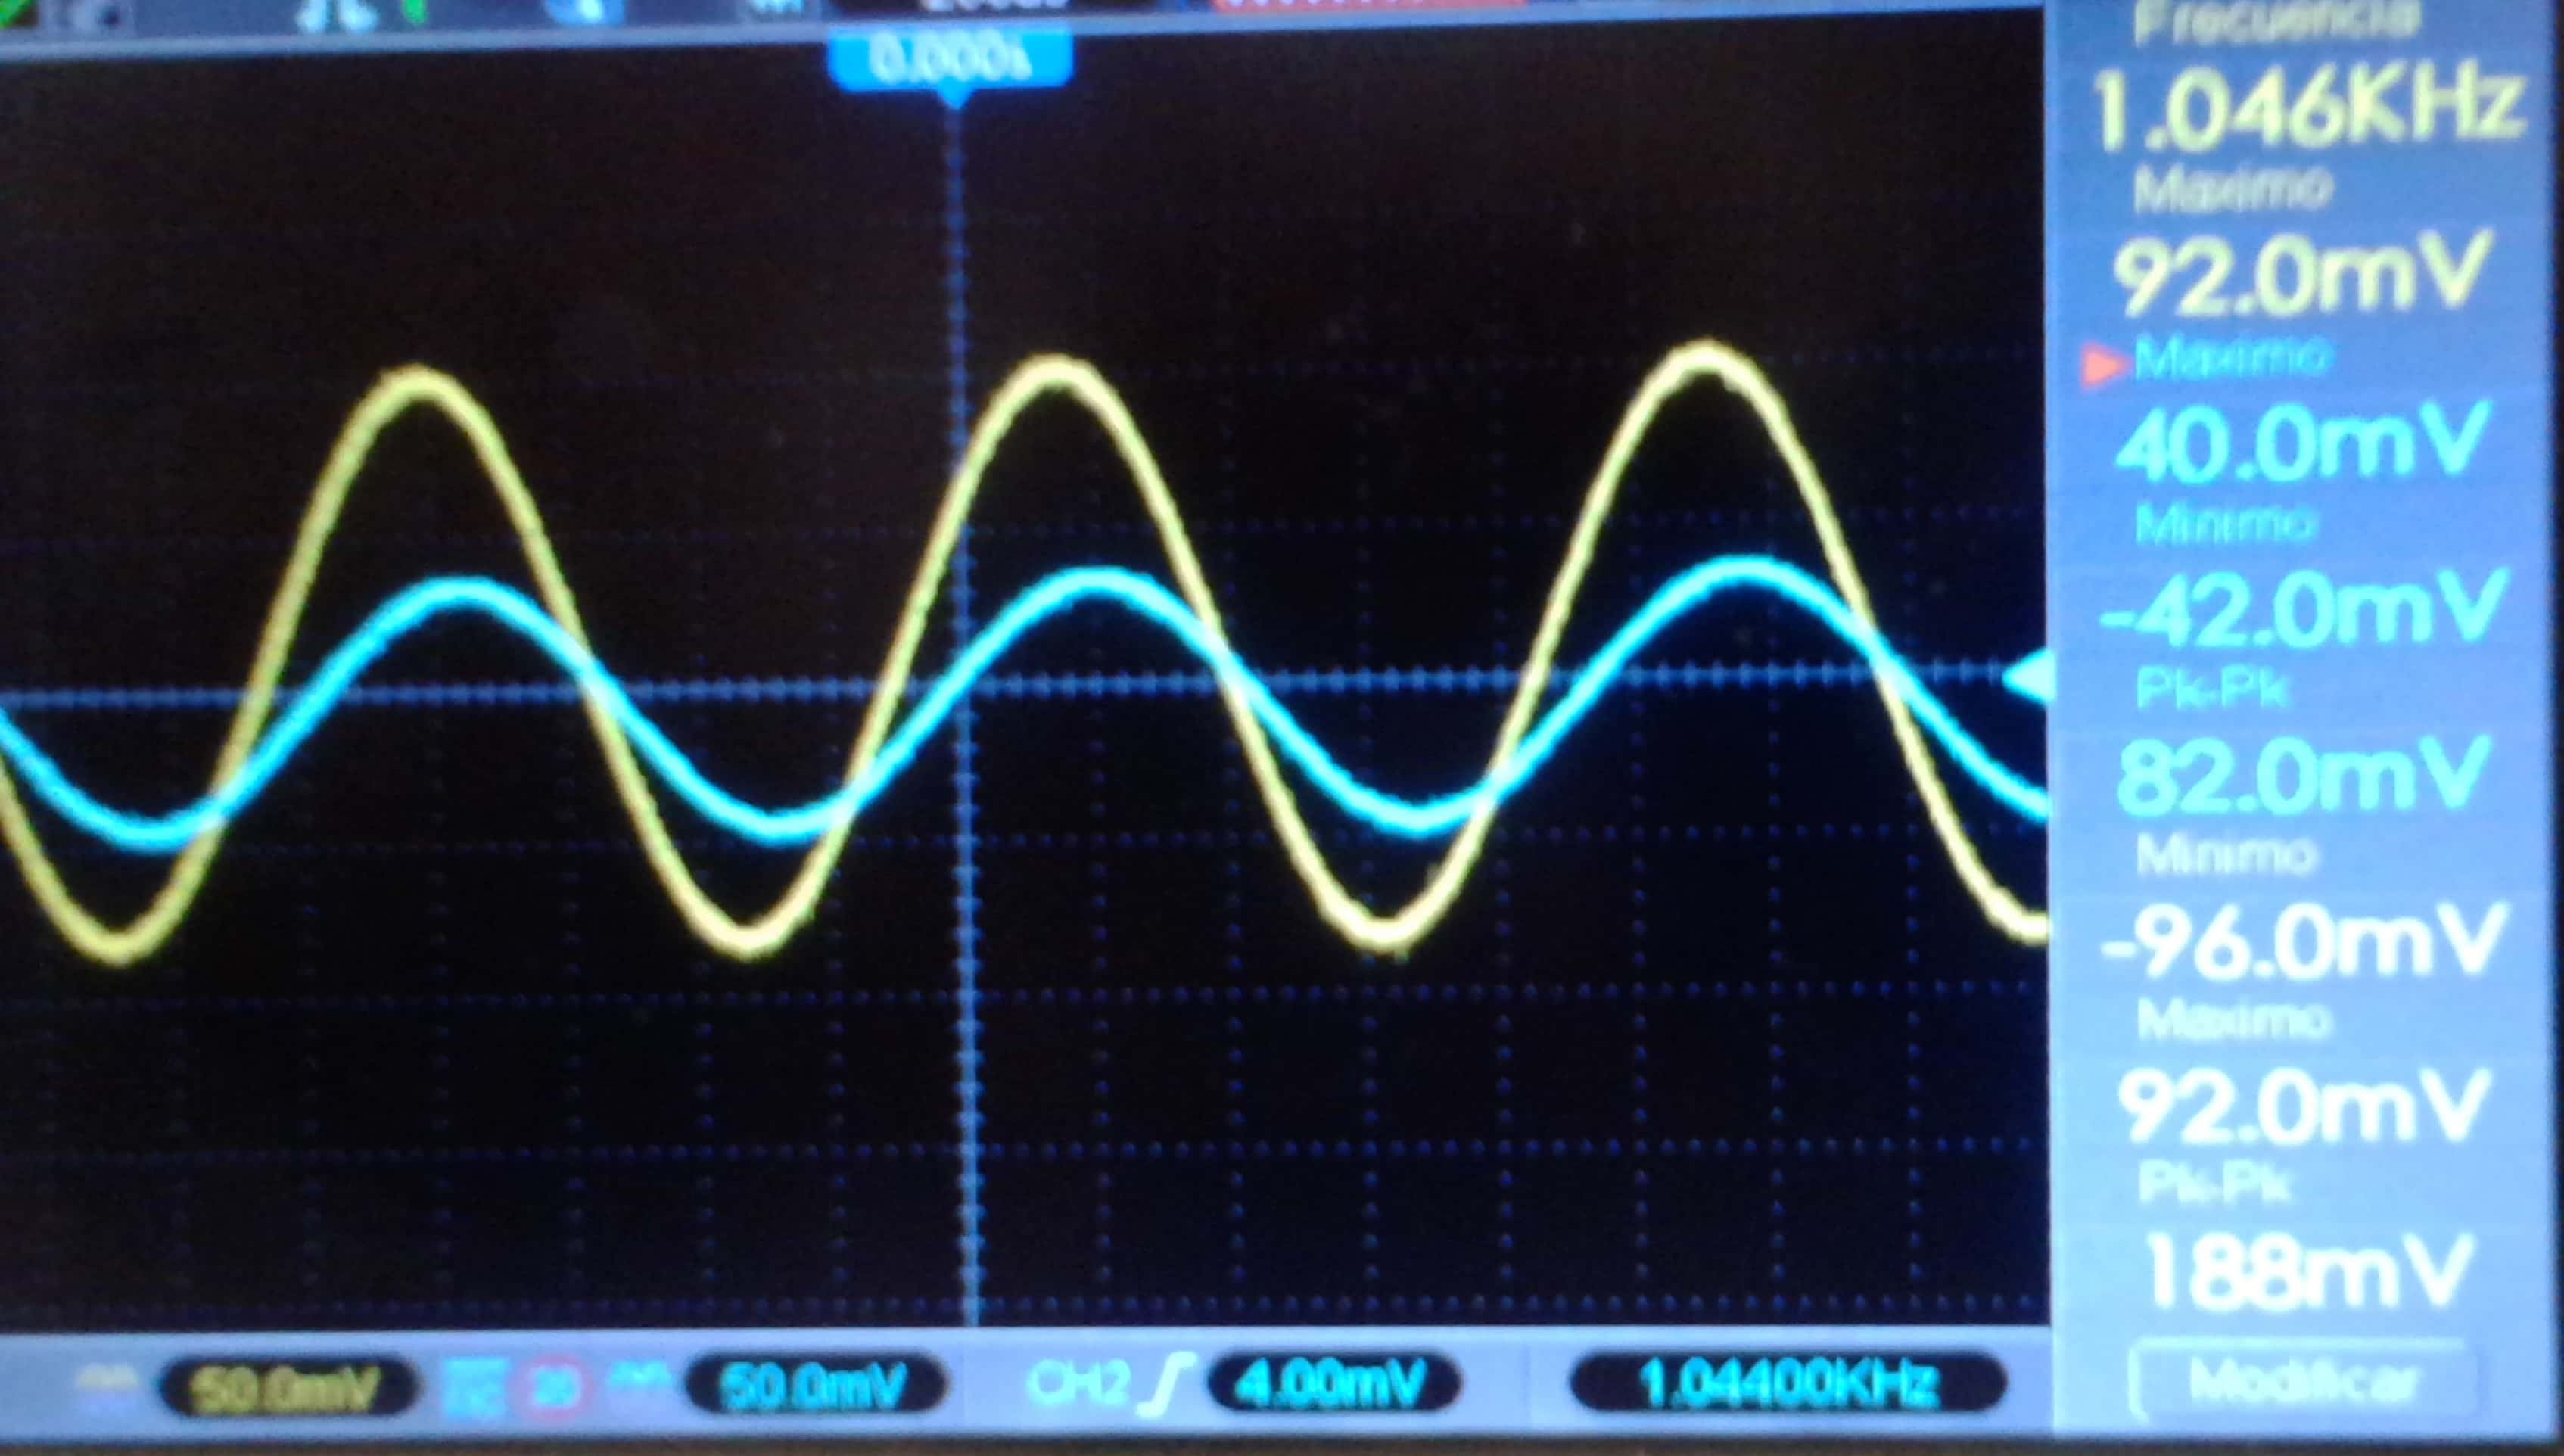
\includegraphics[width=0.8\textwidth]{./Mediciones/Rin_1k.jpg}
			\caption{Medición de las tensiones de generador de prueba y el nodo de entrada.}
			\label{fig:rin_med}
		\end{figure}

		\begin{figure}[ H]
			\centering
			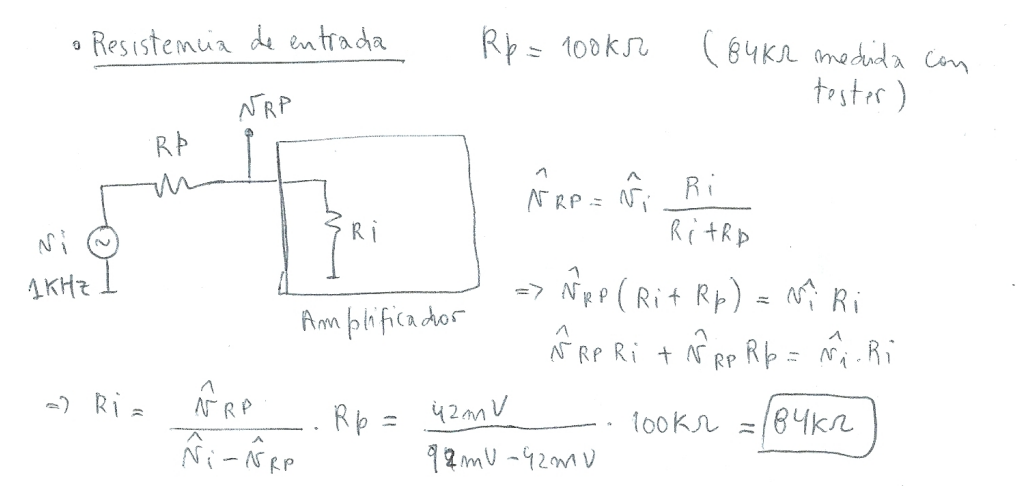
\includegraphics[width=1.0\textwidth]{./Mediciones/Rin_1k_calculo.png}
			\caption{Análisis detallado de la medición de $R_{in}$.}
			\label{fig:analisis_rin_med}
		\end{figure}

		Para la medición de resistencia de entrada, se inyecta una señal conocida al circuito con resistencia serie lo más similar posible a la resistencia de entrada propia del amplificador. La tensión medida está relacionada con el divisor resistivo generado entre $R_{p}$ y $R_{in}$ de forma tal que se puede hallar indirectamente dicha resistencia. La medición se expone en la Figura \ref{fig:rin_med} y en la Figura \ref{fig:analisis_rin_med} se realiza la explicación y cálculo de dicha resistencia resultando $\boxed{R_{in}=\SI{84}{\kilo\ohm}}$.\\

		Del mismo modo se realizó la medición de $R_{in}$ para frecuencia de \SI{10}{\kHz} resultando en:
		\begin{equation*}
			R_{in}(@\SI{10}{\kHz})  = \frac{\SI{13.2}{\mV}}{\SI{94}{\mV} - \SI{13.2}{\mV}} \, \SI{100}{\kilo\ohm} = \boxed{\SI{16.3}{\kilo\ohm}}
		\end{equation*}
		\subsubsection{Ancho de banda de potencia}

	\graficarEPS{1.0}{Mediciones/graf_BW_pot}{Respuesta en frecuencia para tensiones de entrada $V_{pp} = \SI{1.1}{\V}$.}{fig:pot_BW_med}
		
		A través de la Figura \ref{fig:pot_BW_med} se halla la frecuencia en la cual la respuesta en frecuencia disminuya \SI{3}{\dB}. La frecuencia de corte es por tanto:
		\begin{equation*}
			\boxed{f_H \approx \SI{130}{\kHz}}
		\end{equation*}

		\subsubsection{Respuesta al escalón}
		\begin{figure}[h!]
			\centering
			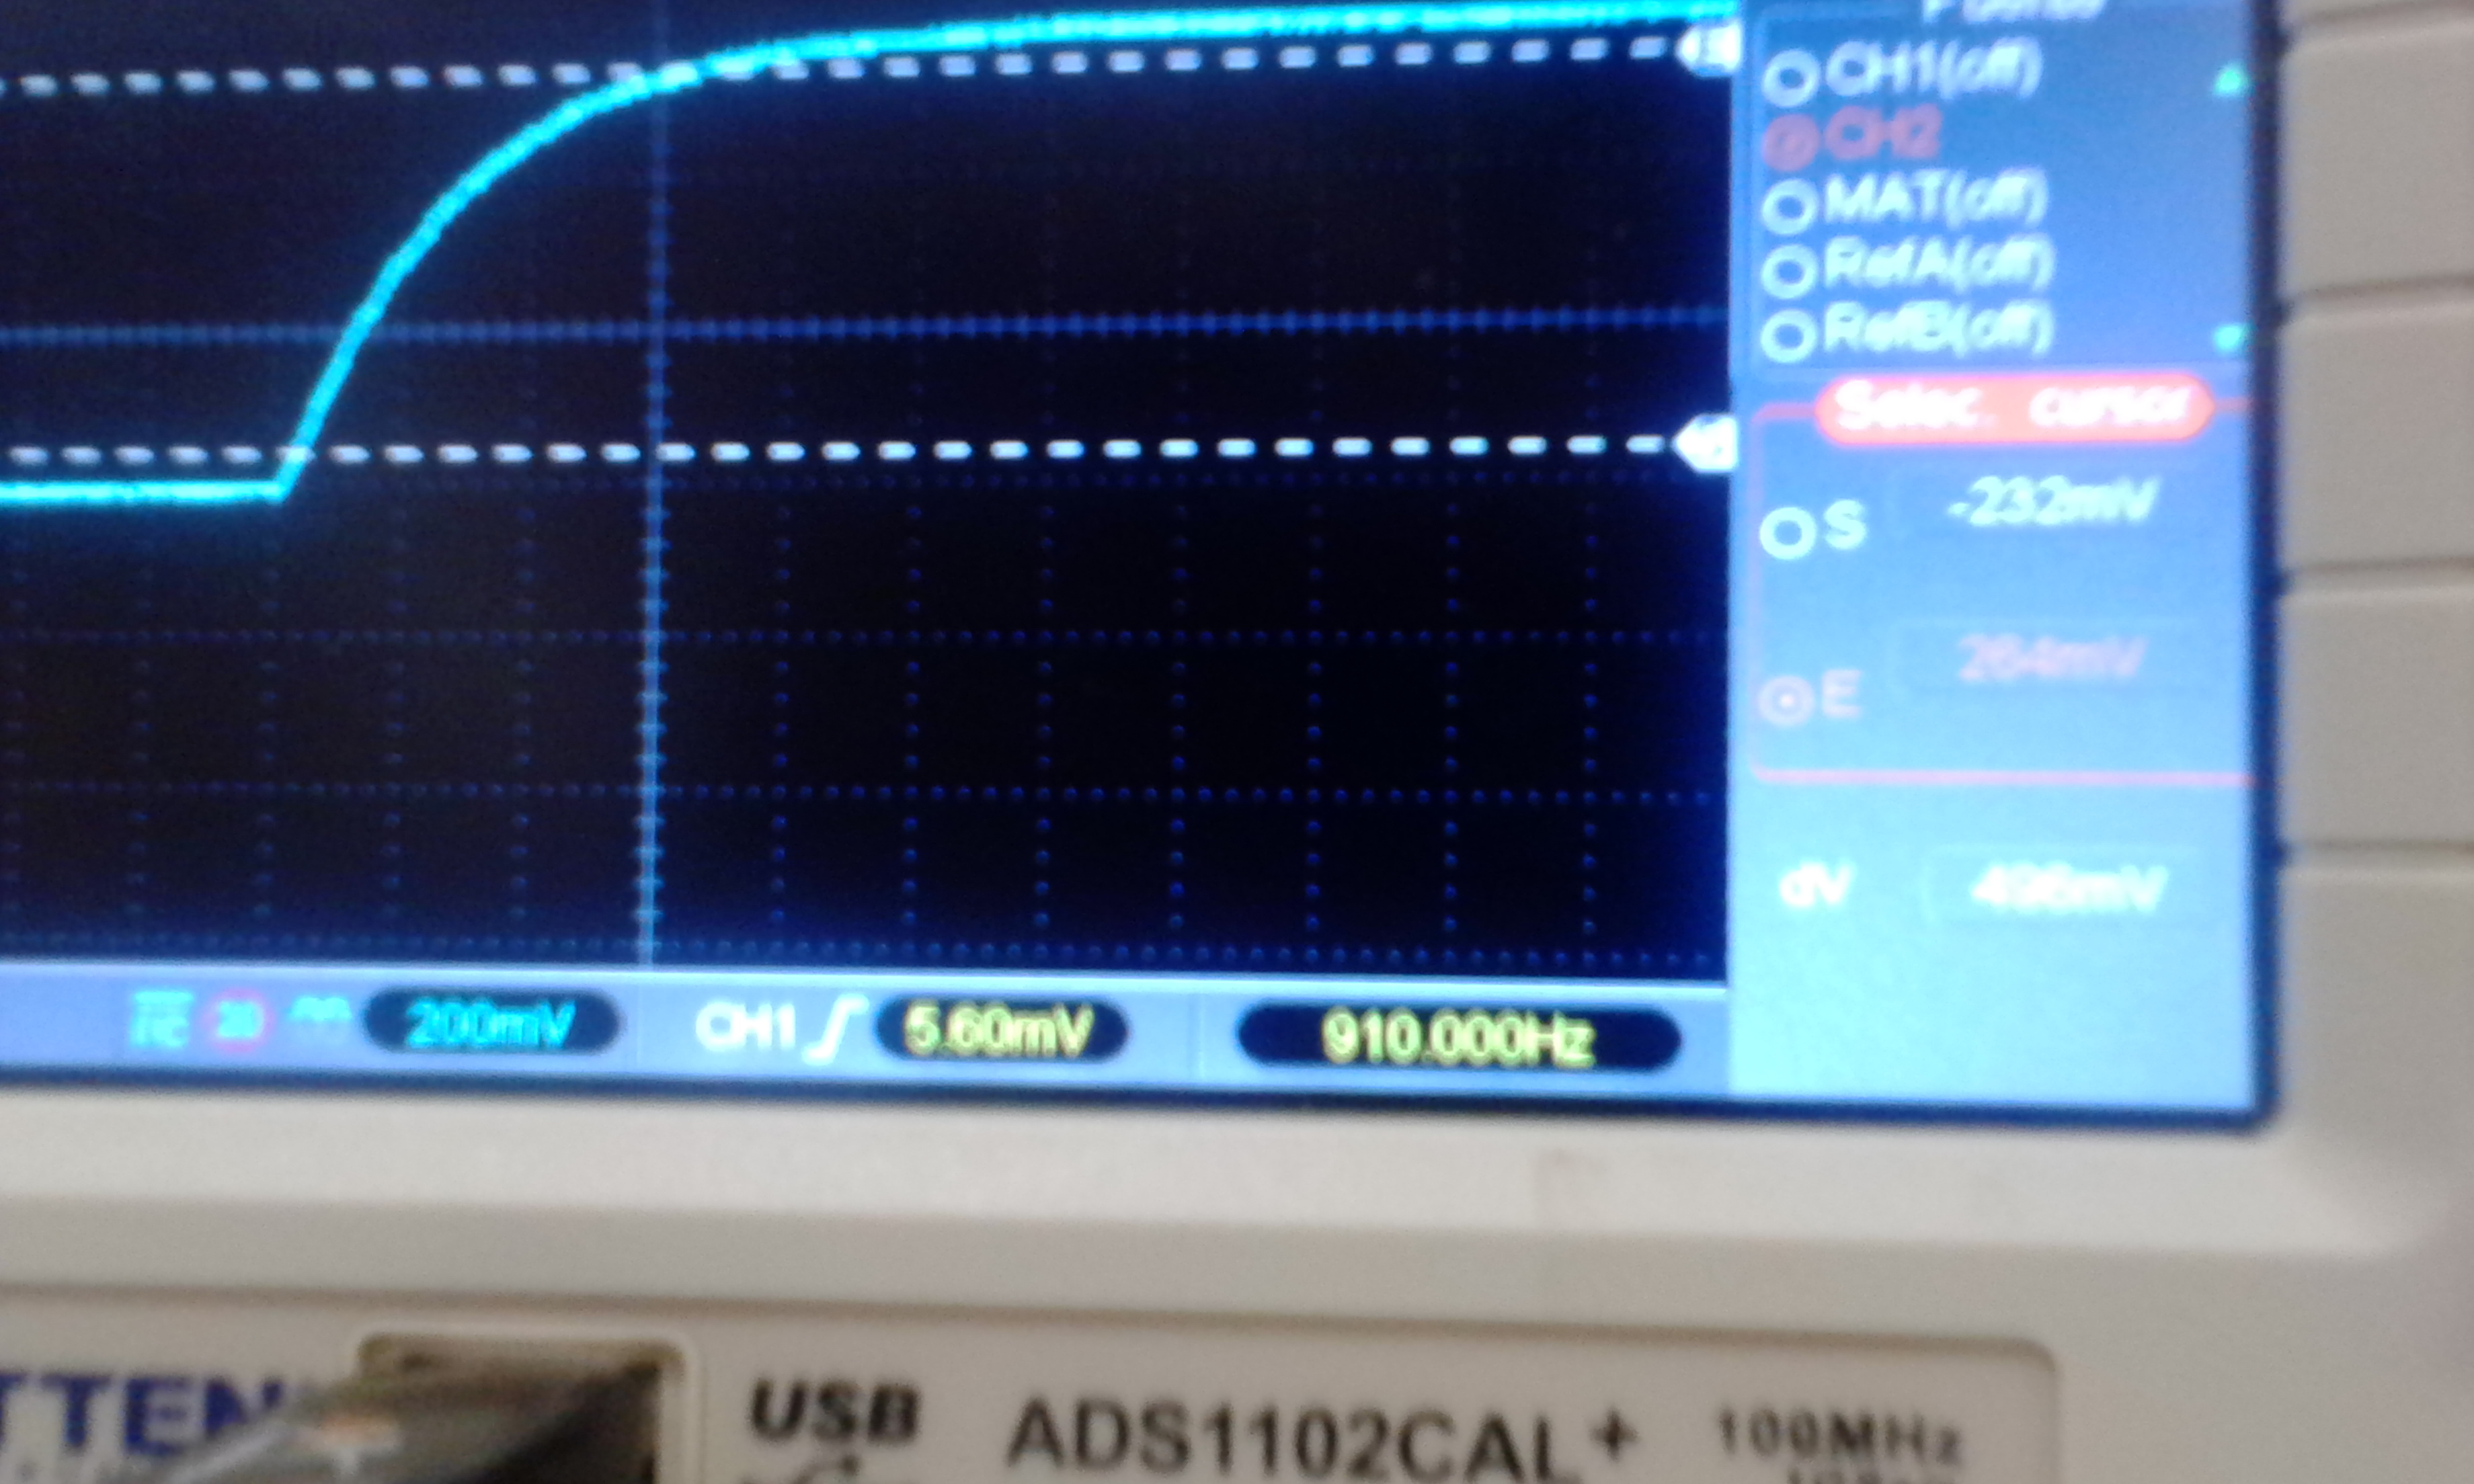
\includegraphics[width=0.8\textwidth]{./Mediciones/BW.jpg}
			\caption{Respuesta al escalón en pequeña señal.}
			\label{fig:escalon_ss}
		\end{figure}

		\begin{figure}[h!]
			\centering
			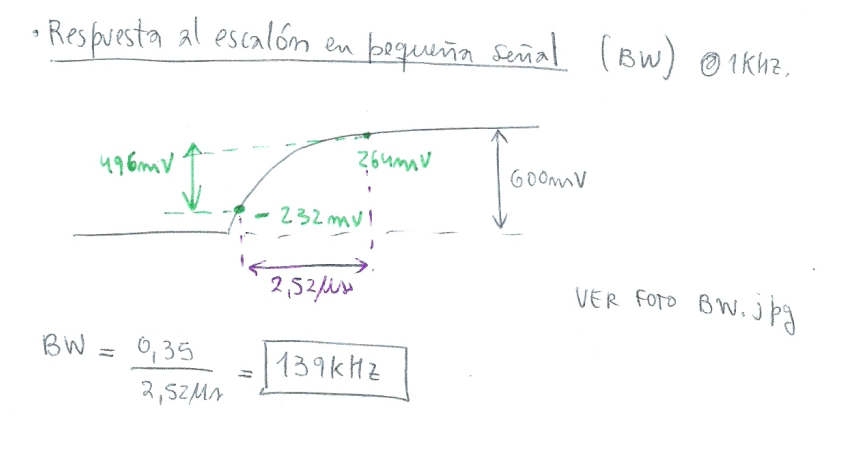
\includegraphics[width=1.0\textwidth]{./Mediciones/BW_calculo.png}
			\caption{Análisis detallado de la medición de respuesta al escalón en señal.}
			\label{fig:analisis_escalon_ss}
		\end{figure}

		Se conecta un generador a la entrada con un escalón de \SI{1}{\kHz}. La medición se expone en la Figura \ref{fig:escalon_ss} y el análisis del mismo se detalla en la Figura \ref{fig:analisis_escalon_ss} resultando en
		\begin{equation*}
			\boxed{BW = \SI{139}{\kHz}}
		\end{equation*}

		\subsubsection{\emph{Slew Rate}}
		Se realiza una medición similar a la anterior, salvo que en este caso la entrada es un escalón que va de \SI{-.6}{\V} a \SI{.6}{\V}. Así a partir de la medición de la Figura \ref{fig:sr_med} como se detallan los valores en la Figura \ref{fig:analisis_sr_med} se obtiene un \emph{Slew Rate} similar al simulado de $\boxed{SR = \SI{8}{\V\per\micro\second}}$.

		\begin{figure}[h!]
			\centering
			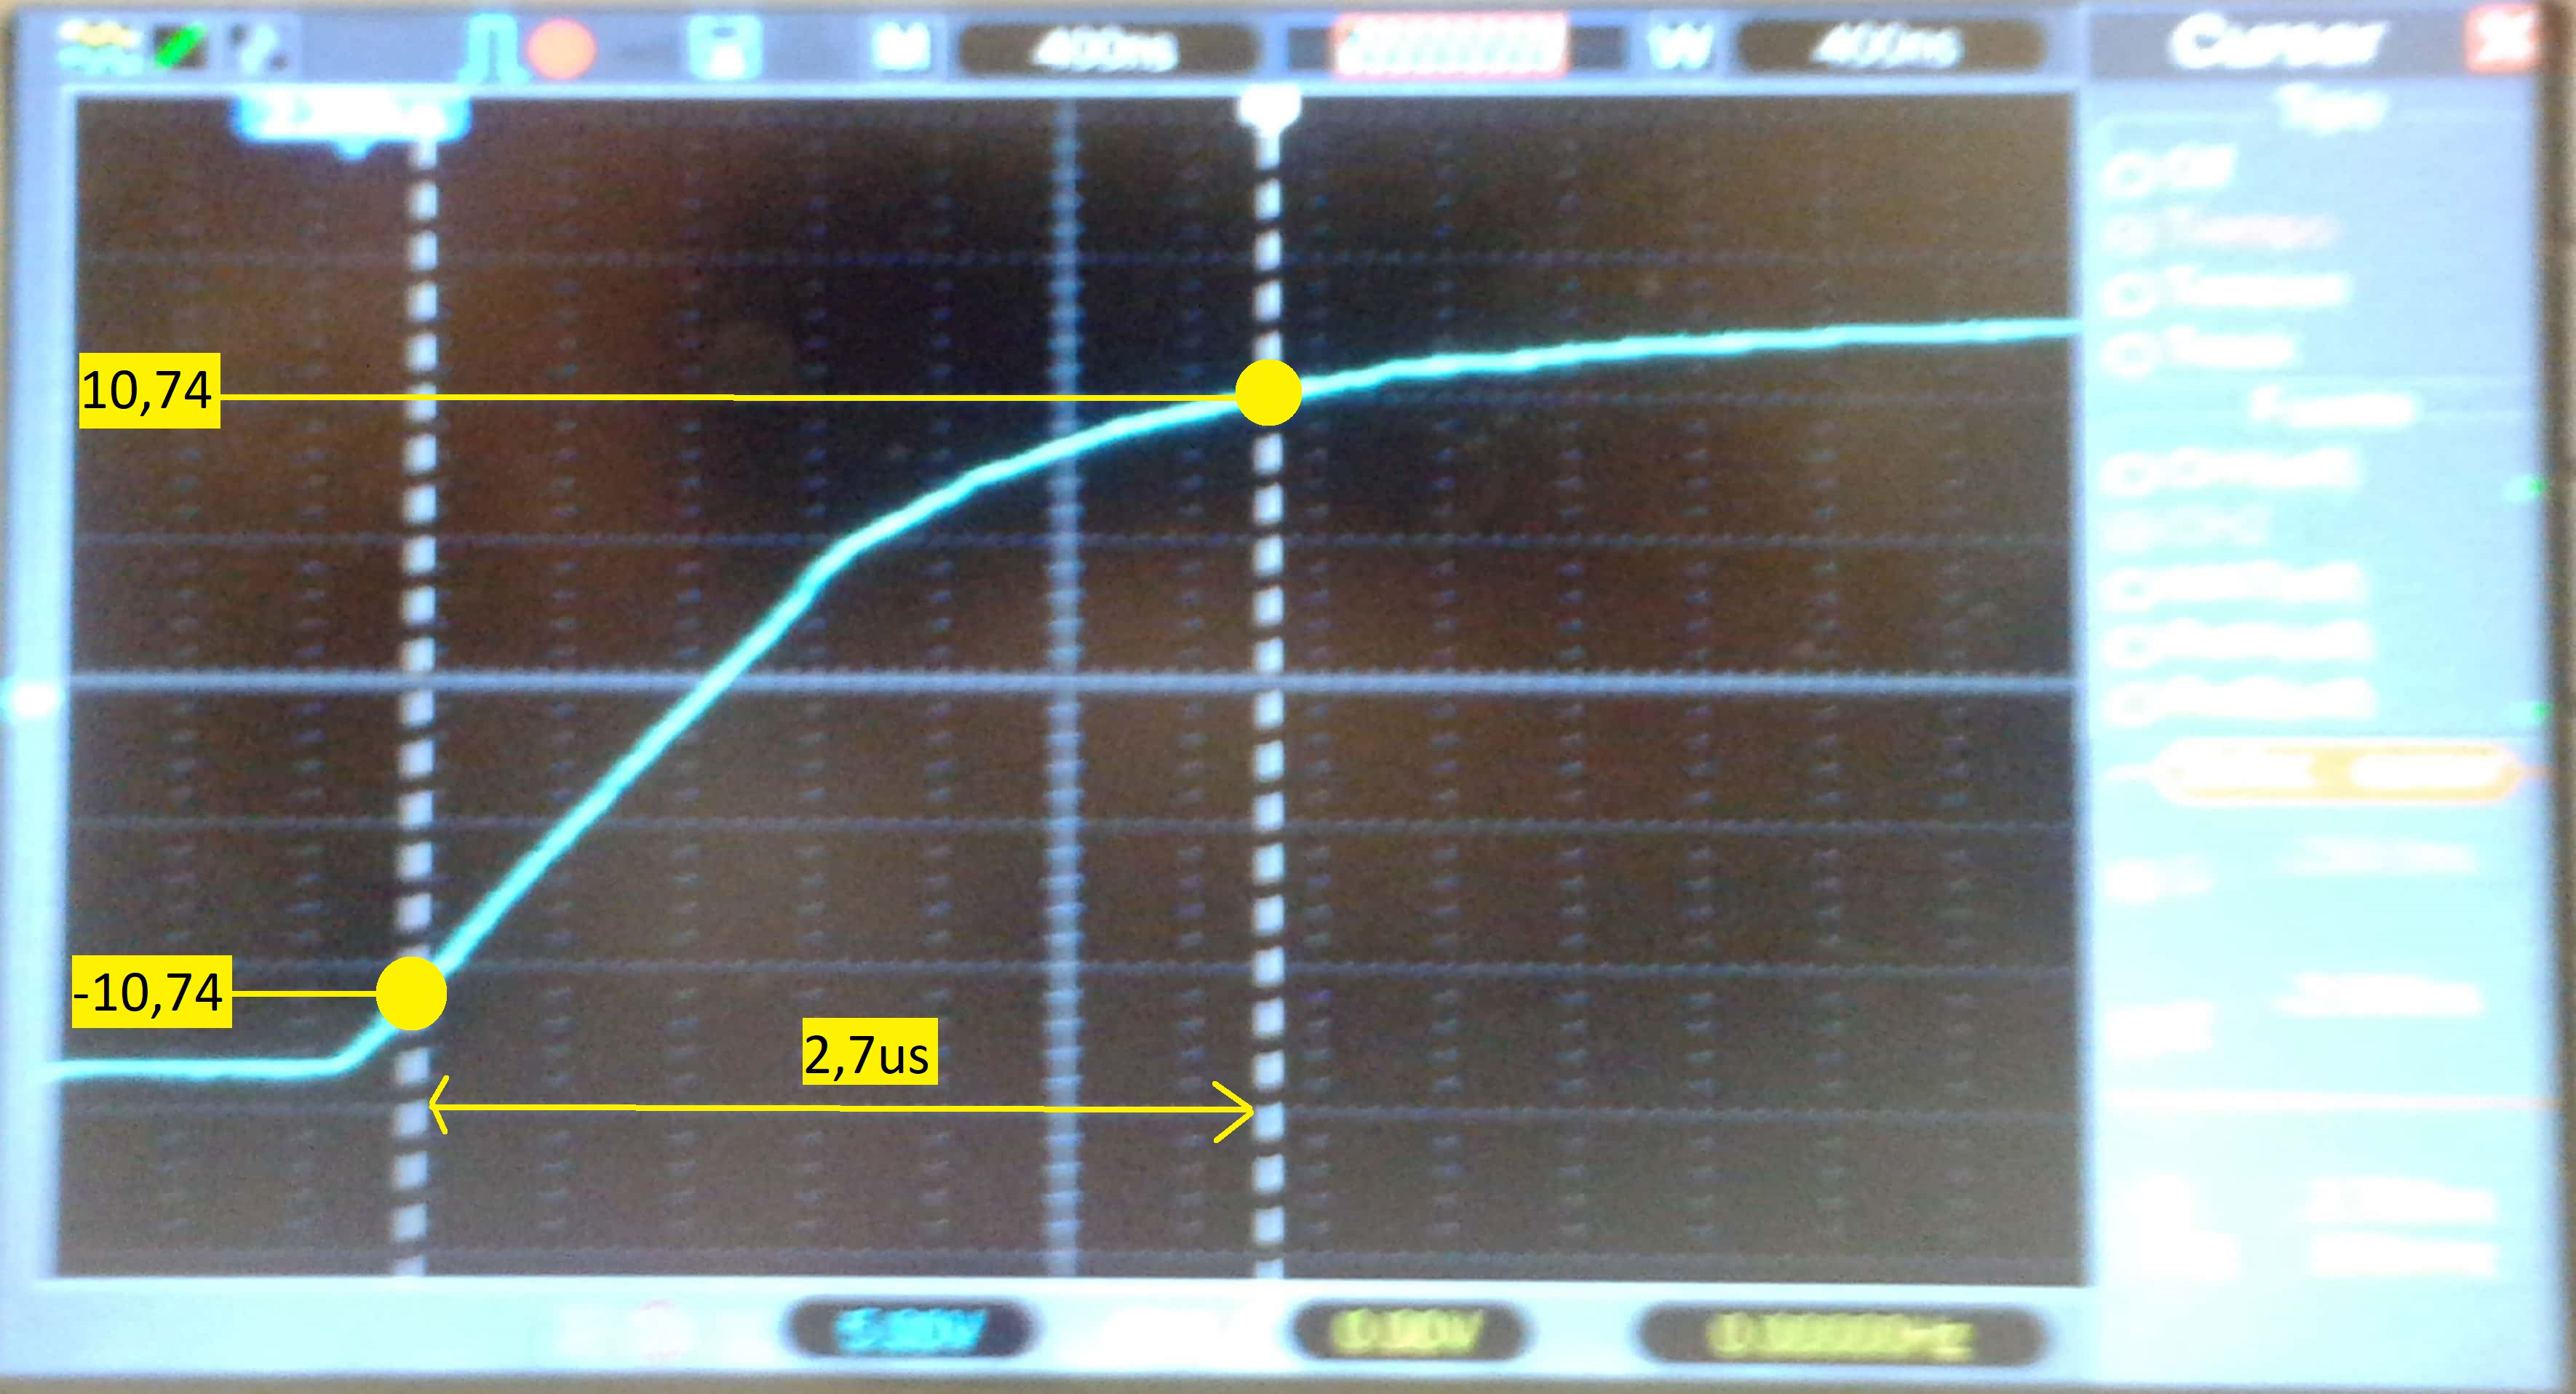
\includegraphics[width=0.8\textwidth]{./Mediciones/SR2.jpg}
			\caption{Respuesta al escalón en gran señal para hallar el \emph{Slew Rate}.}
			\label{fig:sr_med}
		\end{figure}

		\begin{figure}[h!]
			\centering
			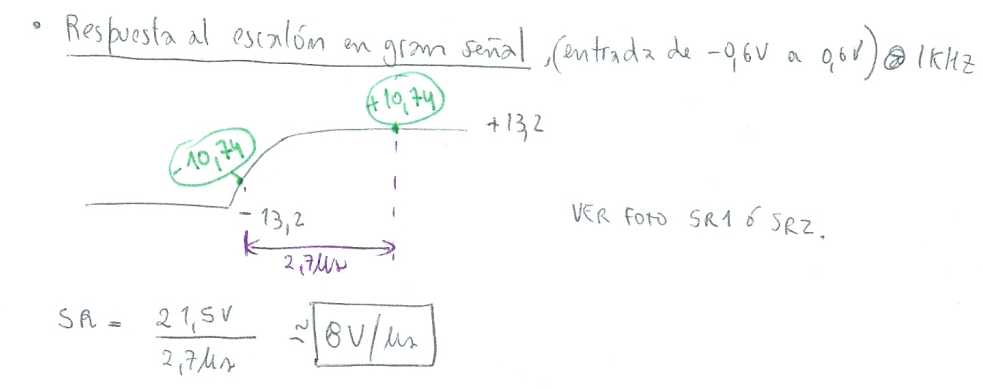
\includegraphics[width=1.0\textwidth]{./Mediciones/SR_calculo.png}
			\caption{Análisis detallado de la medición del \emph{Slew Rate}.}
			\label{fig:analisis_sr_med}
		\end{figure}

		\subsubsection{Variación de la Fuente de Alimentación}
		
		\graficarPNG{0.4}{./Mediciones/Variacion_fuente}{Mediciones de las caídas de potencial para 2 juegos de tensiones de alimentación.}{fig:var_fuente_med}
		En este caso se alimentó el circuito con $V_{CCH+}$ y $V_{CCH-}$ pero se supone que dichas fuentes no son muy buenas. Por tanto se midieron las caídas de potencial sobre las resistencias con los valores de alimentación común y con alimentaciones menores al 10\%. Los resultados y mediciones se exponen en la Figura \ref{fig:var_fuente_med} mostrando errores menores al \num{1.8}\%.


		\subsubsection{Distorsión armónica}
		
			Se realizó un análsis de \emph{FFT} del circuito ingresando con una señal de \SI{1}{\kHz}, pero no se pueden sacar conclusiones de la medición de la Figura \ref{fig:fft_med} porque el piso de ruido es muy alto y no se puede ver el efecto de los harmónicos. Para ello habría que utilizar un \emph{software} que permita ingresar señales particulares y ver el comportamiento en frecuencia del circuito ante esos estímulos.

		\graficarPNG{0.1}{./Mediciones/FFT}{Análisis del circuito por Fourier.}{fig:fft_med}

		\subsubsection{Máxima excursión de salida}
			
		Se introdujo una señal de amplitud tal que la salida no recorte. Dicha señal corresponde a una de amplitud pico a pico \SI{1.1}{\V}. A la salida se obtiene $V_{pp} = \SI{32.4}{\V}$.

		\HgraficarPNG{0.1}{./Mediciones/Maxima_excursion}{Medición de máxima excursión de salida sin recorte.}{fig:excursion_med}

		\subsection{Circuito completo}
		\graficarEPS{0.6}{banco_med_full}{Diagrama del circuito para mediciones con etapa de potencia.}{fig:banco_med_full}
		A continuación se presentan las mediciones realizadas durante la semana del \texttt{18/02/2019}. Se realizó el conexionado del circuito de modo tal que se tiene el circuito completo como se muestra en la Figura \ref{fig:banco_med_full}. 

		%\section{Cambios durante las mediciones}
			%Cortocircuitamos el inductor y la carga en su lugar posta.

			%Medicion slew rate: entramos con \SI{200}{\mV} y \SI{250}{\mV} y frecuencai \SI{1}{\kHz}.

		\subsubsection{Polarización}
			Con el fin de obtener un valor bajo de THD, se ajustó el potenciómetro del multiplicador de $V_{BE}$, obtenéndose los valores de la tabla \ref{tab.valores}.

		\subsubsection{Máxima excursión}
		Se introdujo una señal de amplitud (máxima) tal que la salida no recorte. Dicha señal corresponde a una
		de amplitud pico a pico 2.14 $V_{pp}$. A la salida se obtiene $V_{pp}$ = 50 V.

		\begin{figure}[h!]
			\centering
			\includegraphics[scale=0.1]{Mediciones/PotenciaMaxima.jpg}
			\caption{Medición de máxima excursión de salida antes del recorte.}
			\label{fig:MaxExcur}
		\end{figure}

		\subsubsection{Variación de la fuente}
		Al variar la fuente de alimentación entre -25 y 33 V, se miden los distintos puntos de polarizacion, tal que las corrientes de polarización no varien mas de un 10 por ciento.
		\begin{table}[]
		\begin{tabular}{|l|l|l|l|l|l|l|l|l|l|l|}
		\hline
		Vcc{[}V{]} & -Vcc{[}V{]} & A{[}V{]} & B{[}V{]} & C{[}V{]} & D{[}V{]} & E{[}V{]} & F{[}mV{]} & G{[}mV{]} & H{[}V{]} & I{[}mV{]} \\ \hline
		30.11      & 30          & 12.36    & 1.369    & -29.07   & 1.31     & -1.275   & 27.3      & 11.8      & 29.43    & 10.6      \\ \hline
		31.24      & 30.99       & 12.39    & 1.364    & -29.68   & 1.308    & -1.271   & 25.5      & 7.6       & 28.12    & 10.5      \\ \hline
		32.71      & 32.56       & 12.4     & 1.362    & -31.24   & 1.310    & -1.275   & 27.2      & 10.6      & 32.06    & 10.6      \\ \hline
		24.98      & 25          & 12.06    & 1.358    & -23.69   & 1.309    & -1.270   & 24.6      & 6.3       & 24.37    & 9.9       \\ \hline
		26.99      & 27.02       & 12.18    & 1.363    & -25.7    & 1.309    & 1.27     & 26.1      & 9.6       & 26.37    & 10.3      \\ \hline
		28.39      & 28.18       & 12.25    & 1.363    & -26.86   & 1.311    & -1.27    & 27.1      & 10.2      & 27.75    & 9.2       \\ \hline
		29.21      & 29.13       & 12.29    & 1.363    & -27.82   & 1.311    & -1.275   & 26.2      & 10.4      & 28.58    & 9.3       \\ \hline
		\end{tabular}
		\label{tab.valores}
		\end{table}

		En el esquema \ref{fig:esq_med} se marcan los puntos correspondientes a las mediciones de polarización de la tabla \ref{tab.valores}.

		\begin{figure}[H]
			\centering
			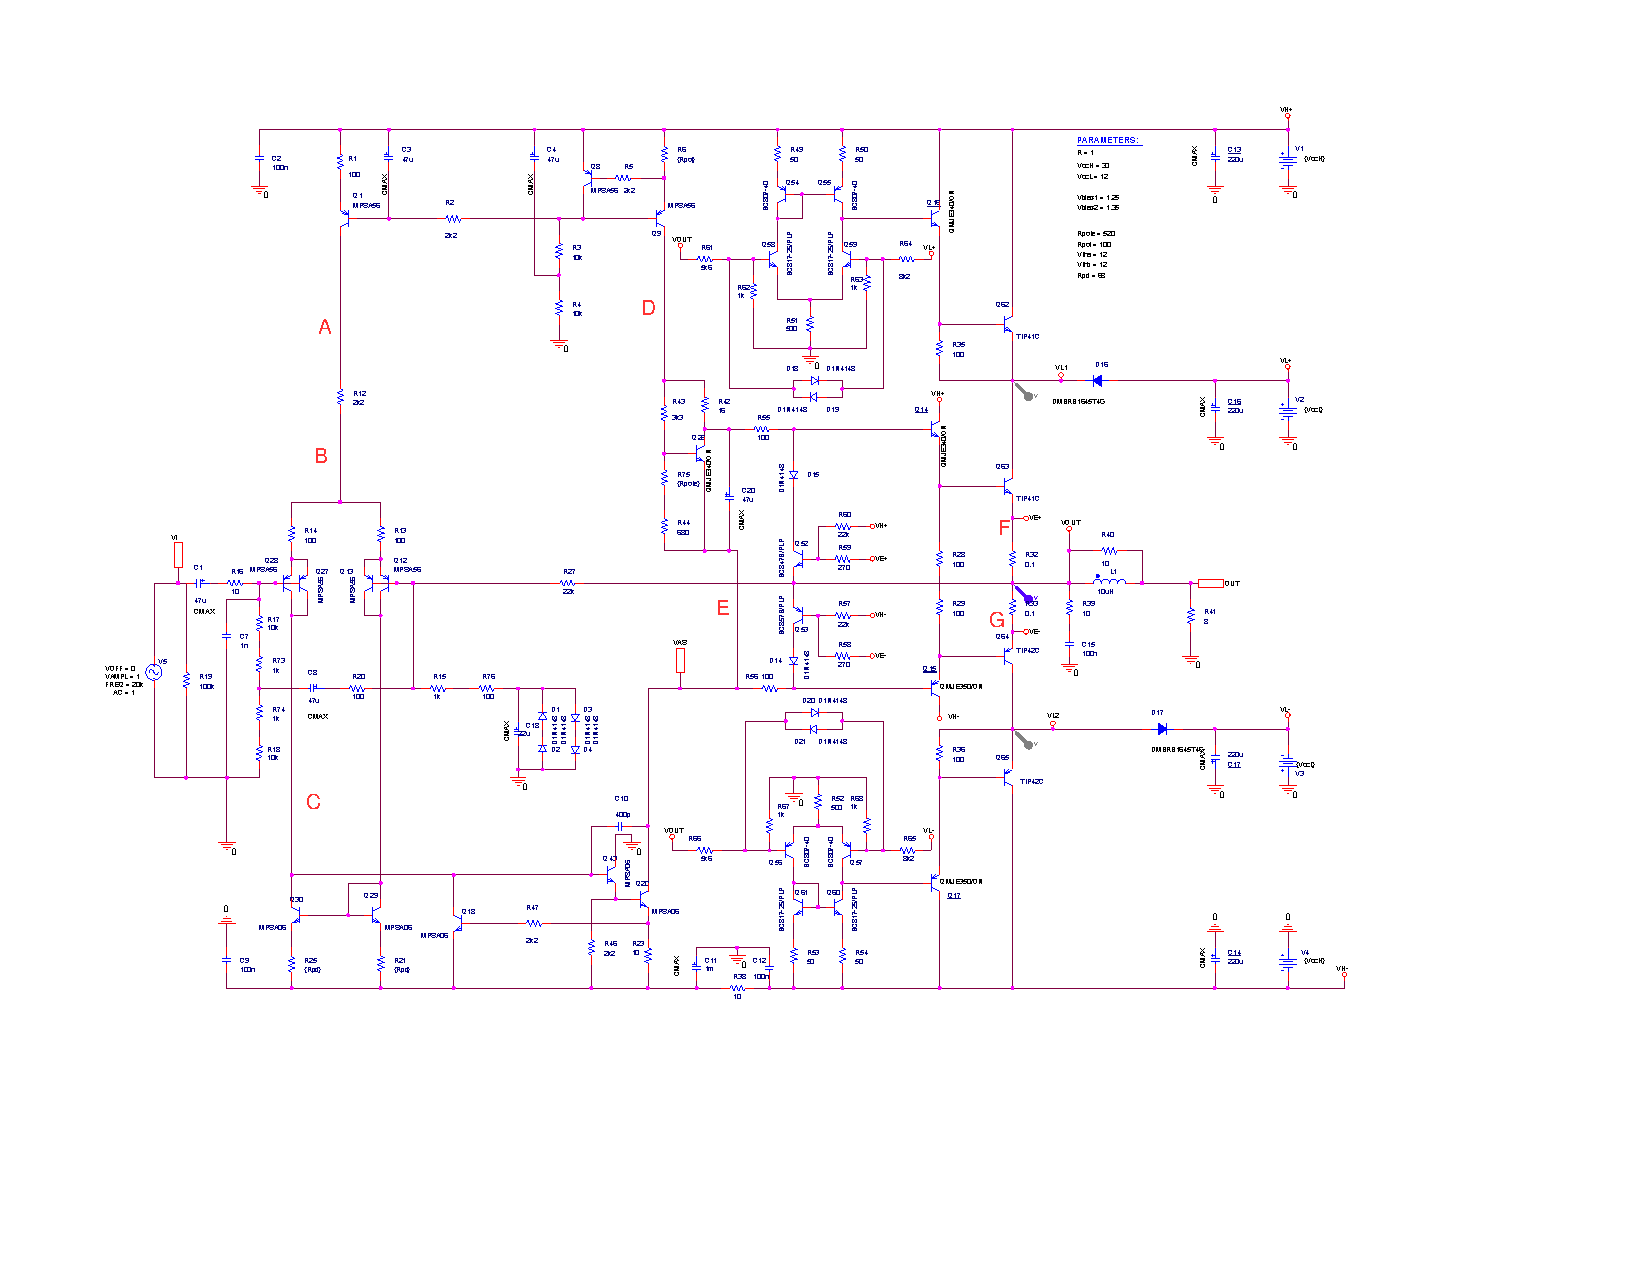
\includegraphics[scale=0.6]{./Figuras/esquema_puntos.pdf}
			\caption{Puntos de medición.}
			\label{fig:esq_med}
		\end{figure}

		\Gus{hay que calcular las corrientes y sus variaciones}
		\subsubsection{Distorsión total armónica}

		El banco de medición para la distorsión total armónica se muestra en la figura \ref{fig:thd_bco}. Los valores se obtuvieron mediante el software \textit{SpectraPlus}. Se utilizó la placa de audio de la PC para generar la señal, ya que un generador de laboratorio presenta un valor elevado de \texttt{THD}. Asimismo es necesario utilizar un atenuador resistivo debido a que la PC no admite como entrada un valor mayor a 1Vrms. 

		\begin{figure}[h!]
			\centering
			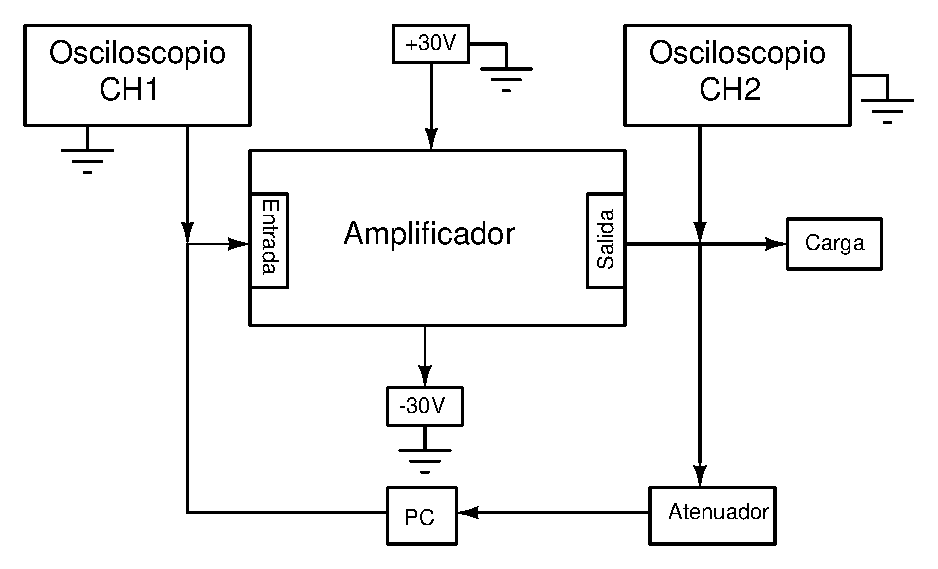
\includegraphics[scale=0.6]{./Figuras/banco_thd.eps}
			\caption{Banco de medición de \texttt{THD}.}
			\label{fig:thd_bco}
		\end{figure}

		\begin{figure}[H]
			\centering
			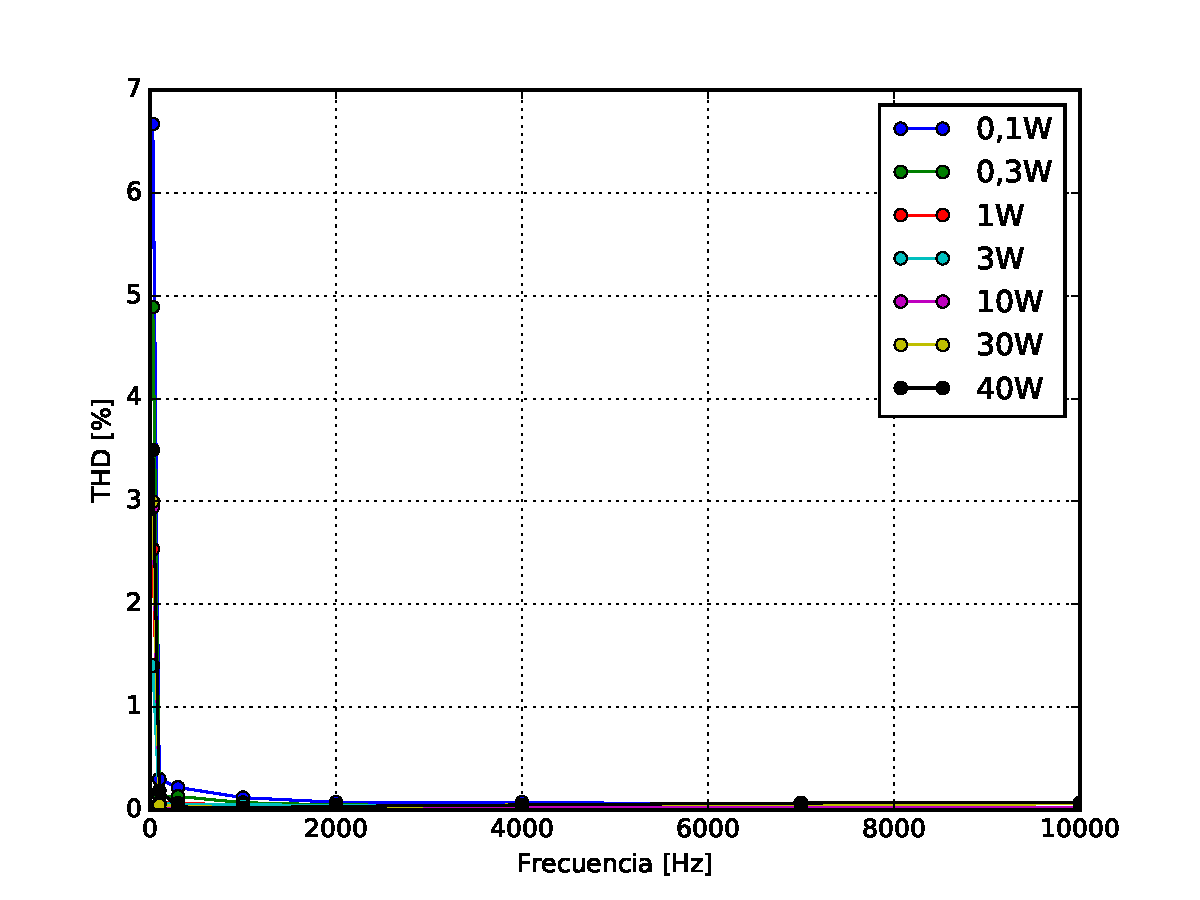
\includegraphics[scale=0.6]{./Figuras/thd.pdf}
			\caption{THD en función de la frecuencia.}
			\label{fig:thd}
		\end{figure}

		\begin{figure}[H]
			\centering
			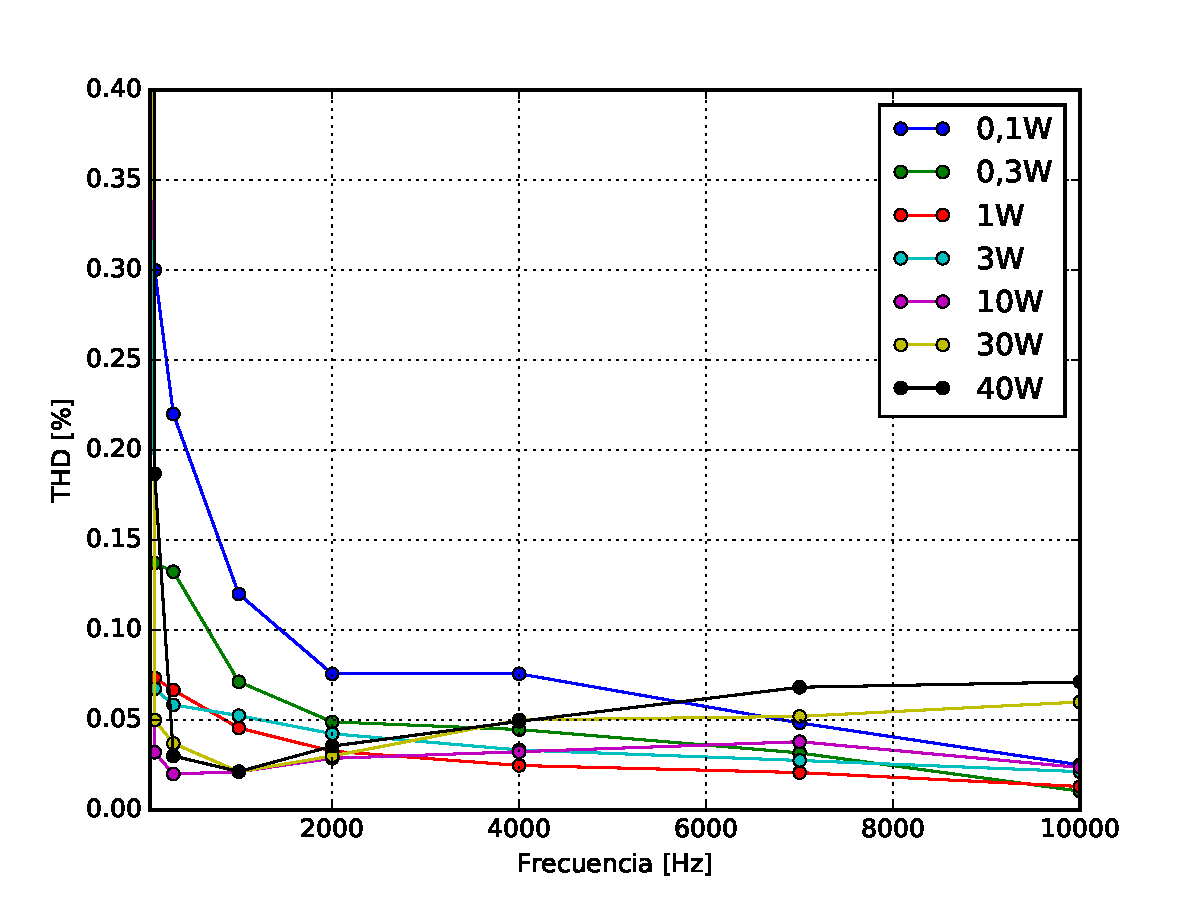
\includegraphics[scale=0.6]{./Figuras/thd_zoom.pdf}
			\caption{THD en función de la potencia.}
		\end{figure}



%		\subsubsection{Compensación}
%
%		\subsubsection{Respuesta en frecuencia}
%
		\subsubsection{Impedancia de salida}
%
%		\subsubsection{Margen de fase}
%
		\subsubsection{Distorsión por intermodulación}

		De manera análoga a la simulación, se calculó la IMD mediante el \textit{software SpectraPlus} con el mismo banco de medición que la Figura \ref{fig:thd_bco}. Las mediciones se realizaron a \SI{5}{\kilo\hertz} para las potencias \SI{0.1}{\watt}, \SI{1}{\watt}, \SI{10}{\watt}

			\begin{table}[H]
				\centering
				\begin{tabular}{cc}
				\toprule
				Potencia [W] & IMD [\%]\\
				\midrule
				0,1 & 0.0593 \\
				1 & 0,0254 \\
				10 & 0,0127 \\
				40 & 0,0253 \\
				\bottomrule
				\end{tabular}
			\end{table}
			%\Flor{Valores para 100 y 5kHz como la simulación. Tambien está 60 7k hecha}



		\subsubsection{Slew-Rate y Ancho de banda de Potencia}
		Se mide a maxima potencia a $1Khz$ y se calcula la pendiente a la salida que se genera por la respuesta al escalón.
		\Gus{Foto}

		\begin{equation*}
			SR  = \frac{\varDelta v}{\varDelta t} = 7.4 \frac{V}{us}
		\end{equation*}

		\subsubsection{Eficiencia}

		\subsection{Respuesta en frecuencia}

		\begin{figure}[H]
			\centering
			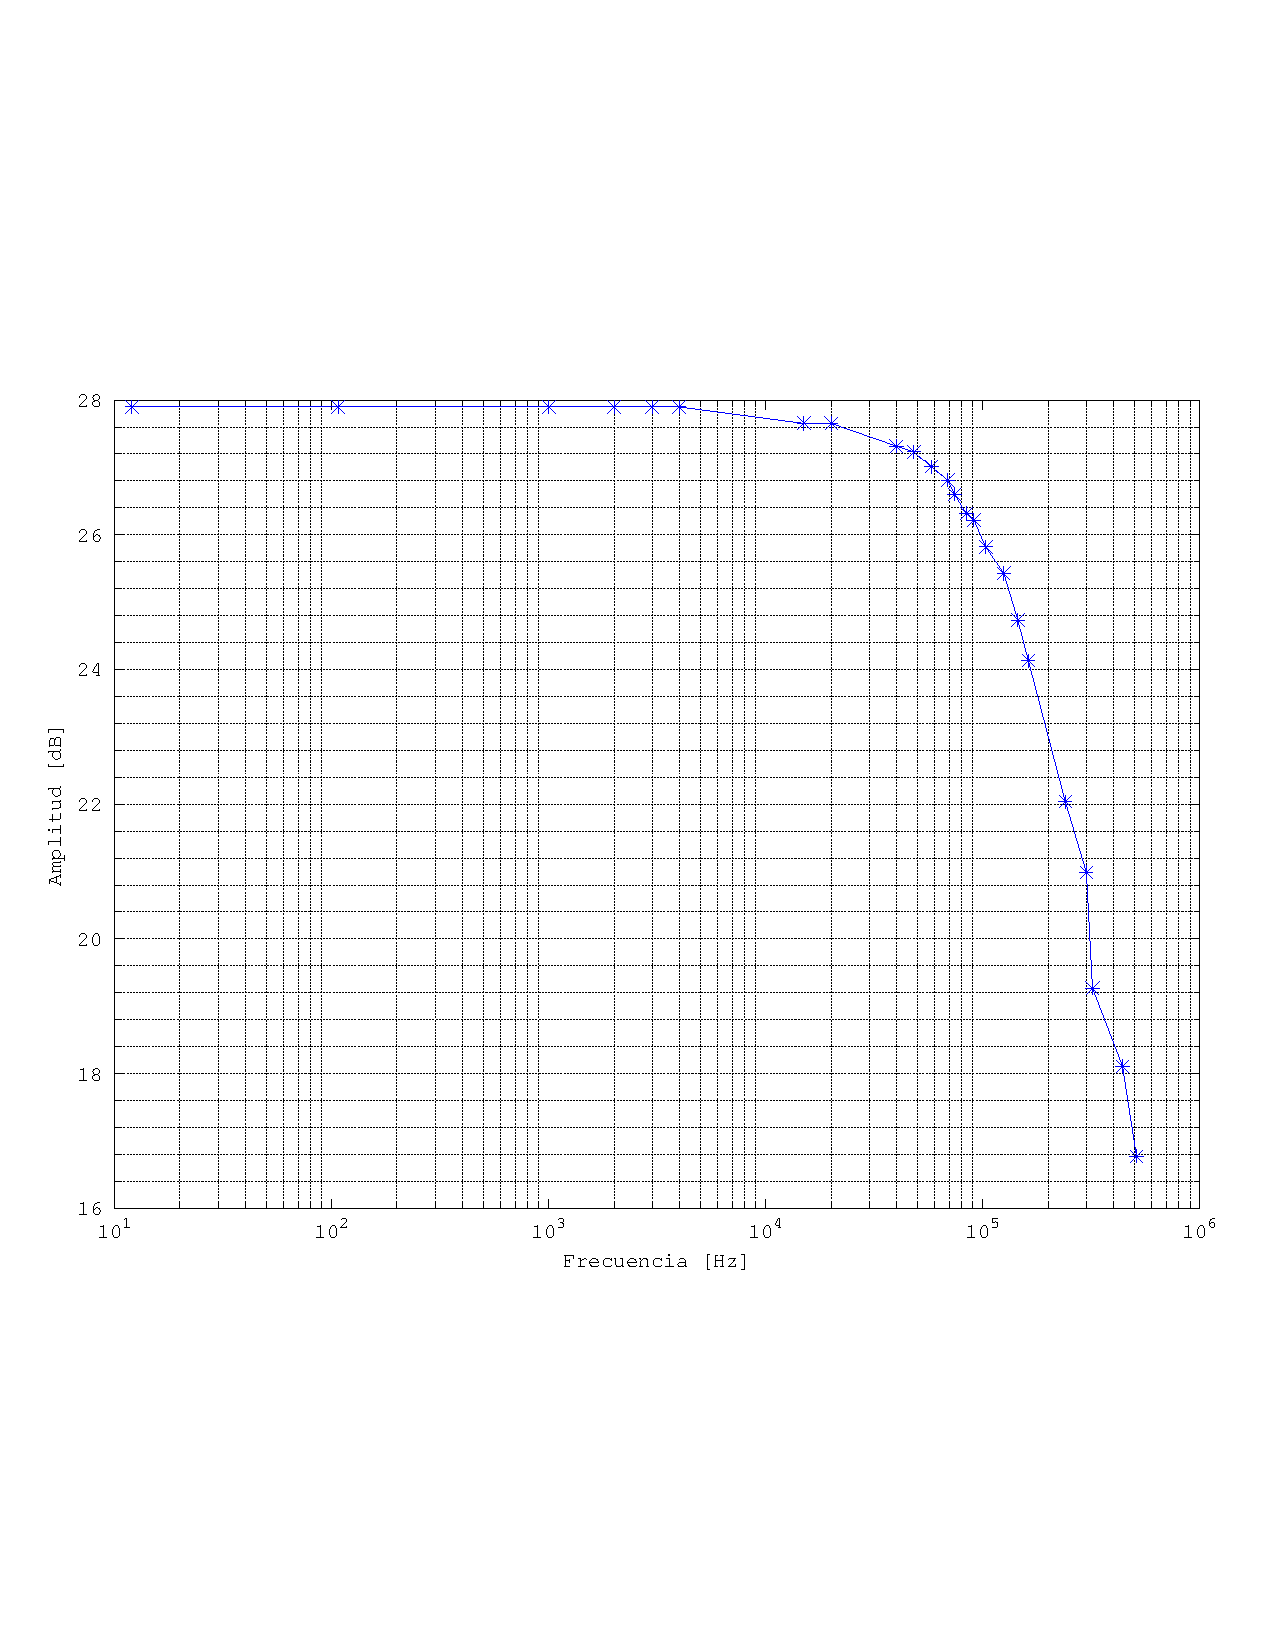
\includegraphics[scale=0.5]{./Figuras/bw_total.pdf}
			\caption{Respuesta en frecuencia a 1W.}
		\end{figure}

		\subsubsection{Relación Señal a Ruido}
		Para realizar la medición de la SNR se utilizó el programa Spectra Plus en el cual se midio con ruido blanco para geerar el piso que presenta la placa de sonido y luego se generó una señal a $1KHz$ y $1W$ midiendo la salida con el banco de medición de la Figura \ref{fig:thd_bco} .



			\begin{figure}[H]
				\centering
				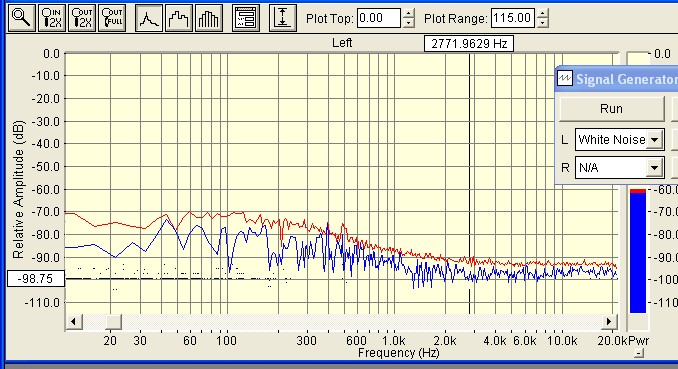
\includegraphics[scale=0.6]{./Figuras/ruido_balnco.jpg}
			\caption{Piso de ruido.}
			\end{figure}

			\begin{figure}[H]
				\centering
				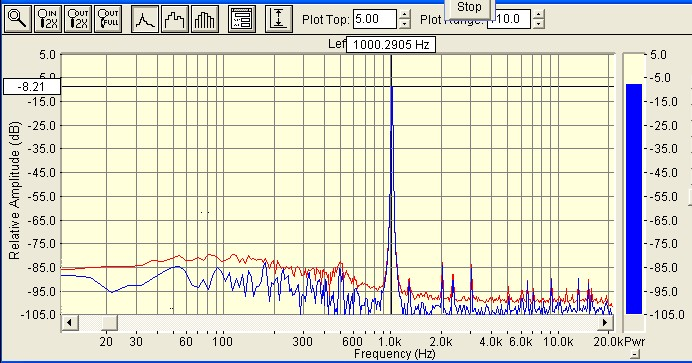
\includegraphics[scale=0.6]{./Figuras/SNR_1K_1W_imagen2.jpg}
			\caption{Salida a 1 W y 1 Khz.}
			\end{figure}


			Calculando:

			\begin{equation*}
			SNR_{db}  = 20 \dot log(\frac{V_{ruido}}{V_o}) = V_{ruido_{dB}} - V_{o_{dB}}
			\end{equation*}

			Por lo tanto: 

			\begin{equation*}
			SNR_{db}  = 98.75 - 8.21 = 90.54 dB  
			\end{equation*}


%		
%		\subsubsection{Rechazo de Ruido de la Fuente de Alimentación}
%
%		\subsubsection{Máxima eficiencia del amplificador}
%
%		\subsubsection{Comportamiento térmico}

			%\input{VII2_valid_ro.tex}
		\section{Validación}
			\begin{table}[H]
	\centering
	\begin{tabular}{cccc}
		\toprule
		& Especificaciones & Simulaciones & Mediciones \\
		\midrule
		THD a $P_{\textit{RMS}} = \SI{40}{\watt}$ @ \SI{1}{\kilo\hertz}& $< \num{0.02}\%$ &  0,018\% & 0,02134\% \\
		THD a \SI{1}{\watt} @ \SI{1}{\kilo\hertz} & $< \num{0.01}\%$ & 0,005\% & 0,04557\%\\
		Respuesta en frecuencia & \SI{20}{\hertz} a \SI{20}{\kilo\hertz} & \SI{14}{\hertz} a \SI{156}{\kilo\hertz} & Hasta \SI{153}{\kHz}\\
		Tensión de \textit{offset} & \SI{5}{\milli\volt} & \SI{2.5}{\milli\volt} & \SI{10}{\milli\volt} \\
		\textit{Slew Rate} & \SI{10}{\volt\per\micro\second} &  \SI{9}{\volt\per\micro\second} & \SI{11.2}{\volt\per\micro\second}\\
		IMD & 1\% & 1,4\% & 0,0253\% \\
		%Margen de Fase & \SI{45}{\degree} &  \SI{45}{\degree} & \\
		Factor de amortiguamiento & $>500$ & 3333 & 89 \\
		Impedancia de entrada & \SI{100}{\kilo\ohm} & \SI{94}{\kilo\ohm} & \SI{84}{\kilo\ohm} \\
		Impedancia de salida & \SI{}{\milli\ohm} & \SI{2.4}{\milli\ohm} & \SI{0.09}{\ohm} \\
		\bottomrule
	\end{tabular}
	\caption{Resultados.}
	\label{tab.resultados}
\end{table}

	\part{Conclusiones}\label{part:conclusiones}
		%En el presente informe se logró analizar el circuito \textit{Turner 730}, obteniéndose resultados semejantes por inspección y simulación.

%La respuesta en frecuencia obtenida resultó ser plana dentro del rango de frecuencias audibles e invariante a la potencia disipada. 

%La eficiencia máxima del circuito (71,2\%) resultó cercana a la ideal (78,5\%), aunque nunca llegará a dicho valor ya que el nodo de salida no puede alcanzar los \SI{30}{\V} (por las caídas de tensión de control de los transistores equivalentes).

%La utilización de un par complementario (\textit{Sziklai}) en vez de un \textit{Darlington} reduce notablemente la distorsión armónica. Pero en el cirucito \textit{Turner 730}, uno de los transistores de etapa de salida es \textit{Darlington}. Esta elección de diseño puede deberse a que en los años 70 los transistores \textit{NPN} y \textit{PNP} no presentaban tanta simetría como hoy en día.


	En el presente informe se logró diseñar un amplificador de audio clase G alternativa, obteniéndose resultados por simulación similares a las especificaciones definidas. La comparación se resume en la Tabla \ref{tab.resultados}. La tensión máxima posible sin distorsión logró llegar a \SI{26.1}{\volt} por simulación, esto produce una potencia sobre la carga de \SI{42.25}{\watt}, por lo que se tiene cierta tolerancia con respecto a la potencia nominal especificada.\\
	\indent A su vez las mediciones realizadas los días \texttt{4/12/18} y \texttt{5/12/18} de las primeras 2 etapas coinciden con los valores obtenidos en el análisis preliminar.





%	\part{Bibliografía}\label{part:bibliografia}
%		\input{IX_bibliografia.tex}

%	\appendix
%	\section{Listado de componentes}
%		\input{A_listado_comp.tex}
\end{document}
